\documentclass[11pt, a4paper]{report}
%----------------------------------------------------------------------------------------
%	PACKAGES (宏包管理)
%----------------------------------------------------------------------------------------
% 1. 编码与语言
\usepackage[english]{babel}
\usepackage[T1]{fontenc}
% 2. 页面布局与排版
\usepackage{geometry}
\geometry{
    textwidth=6in, % 稍微加宽以便放入更好的box
    top=1in,
    bottom=1in,
    headheight=12pt,
    headsep=25pt,
    footskip=30pt
}
\usepackage{setspace}
\setstretch{1.2}
\usepackage{float}
\usepackage{enumitem} % 更好的列表控制
\usepackage{tocloft}  % 加载目录控制宏包
\renewcommand{\cftsecleader}{\cftdotfill{\cftdotsep}} % 强制让 section 后面显示点号
% 3. 数学支持
\usepackage{amsmath, amsthm, amssymb, amsfonts}
\usepackage{mathtools}
\usepackage{thmtools} % 定理环境增强
\usepackage{extarrows}
% 4. 图形与颜色
\usepackage{graphicx}
\usepackage[dvipsnames, svgnames]{xcolor} % 加载更多颜色名
\usepackage{tikz}
\usepackage{tikz-cd}
\usepackage{ytableau} % 杨表
\usetikzlibrary{decorations.pathreplacing, calc, shadows}
\usetikzlibrary{arrows.meta,positioning}

% Define reusable graph styles
\tikzset{
    vertex/.style={circle, fill=black, inner sep=1.5pt, outer sep=0pt},
    graphlabel/.style={align=center, font=\small}
}

% 5. 漂亮的文本框
\usepackage{tcolorbox}
\tcbuselibrary{breakable, skins, theorems}
% 6. 参考文献
%\usepackage[backend=biber,style=gb7714-2015,sorting=gb7714-2015]{biblatex}
%\addbibresource{references.bib}
% 7. 交互 (最后加载)
\usepackage[hidelinks]{hyperref}
\usepackage{array}
%----------------------------------------------------------------------------------------
%	CUSTOM COLORS (自定义配色方案)
%----------------------------------------------------------------------------------------
% 定理色系 - 蓝色
\definecolor{ThmColor}{RGB}{0, 71, 171}        % 深钴蓝
\definecolor{ThmBg}{RGB}{240, 244, 255}        % 极浅蓝
% 定义色系 - 绿色
\definecolor{DefColor}{RGB}{0, 100, 0}         % 深绿
\definecolor{DefBg}{RGB}{240, 255, 240}        % 蜜瓜绿
% 引理/命题色系 - 橙色
\definecolor{LemColor}{RGB}{204, 85, 0}        % 焦橙色
\definecolor{LemBg}{RGB}{255, 248, 240}        % 极浅橙
% 示例/注记色系 - 灰色/紫色
\definecolor{ExColor}{RGB}{105, 105, 105}      % 暗灰
\definecolor{ExBg}{RGB}{250, 250, 250}         % 极浅灰
% 专题/话题色系 - 靛紫色
\definecolor{TopicColor}{RGB}{75, 0, 130}      % 靛蓝色 (Indigo)
\definecolor{TopicBg}{RGB}{248, 245, 255}      % 极浅紫
%----------------------------------------------------------------------------------------
%	THEOREM ENVIRONMENTS (环境美化核心)
%----------------------------------------------------------------------------------------
% 1. Theorem (蓝色风格)
\declaretheorem[name=Theorem, numberwithin=section]{theorem}
\tcolorboxenvironment{theorem}{
    enhanced jigsaw,
    colframe=ThmColor,       % 边框颜色
    colback=ThmBg,           % 背景颜色
    coltitle=white,
    boxrule=0.5pt,           % 边框粗细
    leftrule=2pt,            % 左边框加粗
    sharp corners=downhill,  % 样式
    breakable,               % 允许跨页
    drop shadow=black!5!white % 轻微阴影
}
% Corollary 使用与 Theorem 相同的风格，但通常紧随其后
\declaretheorem[name=Corollary, numberlike=theorem]{corollary}
\tcolorboxenvironment{corollary}{
    enhanced jigsaw,
    colframe=ThmColor!80!white,
    colback=ThmBg,
    boxrule=0pt, leftrule=2pt, arc=0pt, outer arc=0pt,
    breakable
}
% 2. Definition (绿色风格)
\declaretheorem[name=Definition, numberlike=theorem]{definition}
\tcolorboxenvironment{definition}{
    enhanced jigsaw,
    colframe=DefColor,
    colback=DefBg,
    boxrule=0.5pt, leftrule=2pt,
    sharp corners=downhill,
    breakable,
    drop shadow=black!5!white
}
% 3. Lemma & Proposition (橙色风格)
\declaretheorem[name=Lemma, numberlike=theorem]{lemma}
\declaretheorem[name=Proposition, numberlike=theorem]{proposition}
\tcolorboxenvironment{lemma}{
    enhanced jigsaw,
    colframe=LemColor,
    colback=LemBg,
    boxrule=0.5pt, leftrule=2pt,
    breakable
}
\tcolorboxenvironment{proposition}{
    enhanced jigsaw,
    colframe=LemColor,
    colback=LemBg,
    boxrule=0.5pt, leftrule=2pt,
    breakable
}
% 4. Example & Remark (简约风格)
\declaretheorem[name=Example, numberlike=theorem]{example}
\declaretheorem[name=Remark, numberlike=theorem]{remark}
\declaretheorem[name=Exercise, numberlike=theorem]{exercise}
\tcolorboxenvironment{example}{
    enhanced jigsaw,
    colframe=ExColor,
    colback=ExBg,
    leftrule=2pt, boxrule=0pt,
    frame hidden, % 隐藏其他三边
    breakable
}
% 5. Topic (靛紫色风格，带标题支持)
\declaretheorem[name=Topic, numberlike=theorem]{topic}
\tcolorboxenvironment{topic}{
    enhanced jigsaw,
    breakable,
    colframe=TopicColor,        % 边框为靛紫色
    colback=TopicBg,           % 背景为极浅紫
    boxrule=0.5pt,             % 细边框
    leftrule=2pt,              % 左侧加粗线
    sharp corners=downhill,    % 与你其他环境一致的切角样式
    drop shadow=black!5!white, % 轻微阴影
    before skip=15pt,
    after skip=15pt
}
%----------------------------------------------------------------------------------------
%	MATH MACROS (保留你的常用定义)
%----------------------------------------------------------------------------------------
\newcommand{\g}{\mathfrak{g}}
\newcommand{\der}{\mathrm{d}}
\newcommand{\h}{\mathfrak{h}}
\newcommand{\n}{\mathfrak{n}}
\newcommand{\U}{\mathcal{U}}
\newcommand{\C}{\mathbb{C}}
\newcommand{\R}{\mathbb{R}}
\newcommand{\borel}{\mathfrak{b}}
\newcommand{\Ind}{\mathrm{Ind}}
\newcommand{\Hom}{\mathrm{Hom}}
\newcommand{\Ext}{\mathrm{Ext}}
\newcommand{\HRule}[1]{\rule{\linewidth}{#1}}
%----------------------------------------------------------------------------------------
%	TITLE PAGE
%----------------------------------------------------------------------------------------
\begin{document}
\begin{titlepage}
    \centering
    \vspace*{2cm}

    \textsc{\Large Course Notes}\\[0.5cm]

    \HRule{1.5pt} \\[0.5cm]
    { \huge \bfseries Applied Abstract Algebra \\[0.3cm] Quiver Theory }\\[0.4cm]
    \HRule{1.5pt} \\[1.5cm]

    \vspace{3cm}

    % 人员信息区域：垂直排列并区分字号
    \begin{spacing}{1.8}
        {\Large \textbf{Instructor:}} \\
        {\Large Prof. Iryna \textsc{Kashuba}} \\[0.8cm]

        {\normalsize \textit{TA:}} \\
        {\normalsize Leo}
    \end{spacing}

    \vfill
    {\large \today}
\end{titlepage}
\newpage
\tableofcontents
\newpage


%----------------------------------------------------------------------------------------
%    CONTENT STRUCTURE TEMPLATE
%----------------------------------------------------------------------------------------

\chapter{Lecture 1}

\begin{tcolorbox}[
        enhanced,
        title=\textbf{Course Information},
        colframe=TopicColor,
        colback=TopicBg,
        coltitle=white,
        boxrule=0.5pt,
        leftrule=2pt,
        sharp corners=downhill,
        drop shadow=black!5!white
    ]
    \textbf{\textcolor{TopicColor}{Main topic:}} Representation theory of quivers.

    \textbf{\textcolor{TopicColor}{Office hours:}} Mon: 12:30-14:30. Office 218, Taizhou Building.

    \textbf{\textcolor{TopicColor}{Main book:}} \textit{Ralf Schiffler, Quiver Representations}

    \textbf{\textcolor{TopicColor}{References:}}
    \begin{itemize}[leftmargin=*, nosep, label=\textcolor{TopicColor}{$\bullet$}]
        \item \textit{Assem, Simson, Skowro\'{n}ski, Elements of the Representation Theory of Associative Algebras, Vol. 1: Techniques of Representation Theory}, Cambridge University Press.
        \item \textit{Ibrahim Assem, Basic Representation Theory of Algebras}.
        \item \textit{Michel Brion, Representations of Quivers}.
        \item \textit{Henning Krause, Representations of Quivers via Reflection Functor}.
        \item \textit{W. Crawley-Boevey, Lectures on Representations of Quivers}.
        \item \textit{Ralf Schiffler, Quiver Representations}.
        \item \textit{Alexander Kirillov Jr., Quiver Representations and Quiver Varieties}, Graduate Studies in Mathematics, American Mathematical Society, 2016.
    \end{itemize}
    \textbf{\textcolor{TopicColor}{Grading:}}
    \begin{itemize}[leftmargin=*, nosep, label=\textcolor{TopicColor}{$\bullet$}]
        \item Midterm: 30\%
        \item Attendance: 10\%
        \item Homework: 20\%
        \item Final: 40\%
    \end{itemize}
    Midterm will be on April 13th, Monday, 2026 (the 8th week).
\end{tcolorbox}

\section{Quivers}

\begin{definition}
    A quiver $Q$ is a quadruple $(Q_0, Q_1, s, t)$, where $Q_0$ is a set of vertices, $Q_1$ is a set of arrows, and $s, t: Q_1 \to Q_0$ are two maps. For any arrow $\alpha \in Q_1$, $s(\alpha)$ is called the source of $\alpha$ and $t(\alpha)$ is called the target of $\alpha$. For example, if $\alpha: 1 \to 2$, then $s(\alpha)=1$ and $t(\alpha)=2$.
\end{definition}

\begin{example}
    Let $Q_0 = \{1,2,3\}$ and $Q_1 = \{\alpha,\beta,\gamma,\delta\}$.
    We have $s(\alpha)=2, t(\alpha)=2$; $s(\beta)=3, t(\beta)=1$; $s(\gamma)=s(\delta)=1, t(\gamma)=t(\delta)=2$.
    \begin{center}
        \begin{tikzcd}
            \underset{\bullet}{1} \arrow[r, "\gamma", bend left] \arrow[r, "\delta"', bend right] & \underset{\bullet}{2} \arrow["\alpha"', loop, distance=2em, in=305, out=235] & \underset{\bullet}{3} \arrow[ll, "\beta"', bend right=49]
        \end{tikzcd}
    \end{center}
    Let $\xi = \alpha \gamma \beta$ be a path. Then $s(\xi)=s(\beta)=3$ and $t(\xi)=t(\alpha)=2$.
\end{example}

\begin{example}
    Jordan quiver.
    The Jordan quiver consists of a single vertex and a single arrow starting and ending at this vertex. Formally, $Q_0 = \{1\}$ and $Q_1 = \{\alpha\}$ with $s(\alpha) = t(\alpha) = 1$.
    It is called the Jordan quiver because its representations correspond to vector spaces equipped with a linear endomorphism. The classification of such representations up to isomorphism is equivalent to the classification of square matrices up to similarity, which is given by the Jordan normal form theorem (over an algebraically closed field).
    \begin{center}
        \begin{tikzcd}
            \bullet \arrow[loop, distance=2em, in=125, out=55]
        \end{tikzcd}
    \end{center}
\end{example}

\begin{example}
    $r$-Kronecker quiver.
    The $r$-Kronecker quiver has two vertices, say 1 and 2, and $r$ arrows $\alpha_1, \dots, \alpha_r$ from 1 to 2. Thus $Q_0 = \{1, 2\}$, $Q_1 = \{\alpha_1, \dots, \alpha_r\}$, with $s(\alpha_i) = 1$ and $t(\alpha_i) = 2$ for all $i=1, \dots, r$.
    It is named after Leopold Kronecker. In the case $r=2$, the representations correspond to pairs of linear maps between two vector spaces, which can be represented by matrix pencils. Kronecker solved the classification problem for these pencils.
    \begin{center}
        \begin{tikzcd}
            1 \arrow[r, "1", bend left=49] \arrow[r, "\ldots", no head, dashed] \arrow[r, "r"', bend right=49] & 2
        \end{tikzcd}
    \end{center}
\end{example}

\begin{example}
    $n$-subspace quiver.
    The $n$-subspace quiver consists of $n+1$ vertices $\{0, 1, \dots, n\}$ and $n$ arrows $\alpha_1, \dots, \alpha_n$ such that $s(\alpha_i) = i$ and $t(\alpha_i) = 0$ for all $i=1, \dots, n$.
    It is called the $n$-subspace quiver because its representations are related to configurations of subspaces. If the linear maps associated with the arrows are injective, a representation corresponds to a collection of $n$ subspaces of the vector space associated with the central vertex.
    \begin{center}
        \begin{tikzcd}
            & \underset{\bullet}{0}            &        &                                    \\
            &                                  &        &                                    \\
            \underset{\bullet}{1} \arrow[ruu] & \underset{\bullet}{2} \arrow[uu] & \ldots & \underset{\bullet}{n} \arrow[lluu]
        \end{tikzcd}
    \end{center}
\end{example}

\begin{definition}[Finite quiver]
    A quiver $Q=(Q_0, Q_1, s, t)$ is called finite if both the set of vertices $Q_0$ and the set of arrows $Q_1$ are finite sets.
\end{definition}

For the base field we assume $k=\bar{k}$. Usually we take $k=\C$.

\section{Representations}

\begin{definition}
    A representation $M$ of a quiver $Q$ consists of a vector space $M_i$ for each vertex $i \in Q_0$ and a linear map $\phi_{\alpha}: M_{s(\alpha)} \to M_{t(\alpha)}$ for each arrow $\alpha \in Q_1$. We denote this representation by $M=(M_i, \phi_{\alpha})_{i \in Q_0, \alpha \in Q_1}$.
\end{definition}

\begin{example}
    For example 1:
    \begin{center}
        \begin{tikzcd}
            \underset{\bullet}{M_1} \arrow[r, "\phi_\gamma", bend left] \arrow[r, "\phi_\delta"', bend right] & \underset{\bullet}{M_2} \arrow["\phi_\alpha"', loop, distance=2em, in=305, out=235] & \underset{\bullet}{M_3} \arrow[ll, "\phi_\beta"', bend right=49]
        \end{tikzcd}
    \end{center}
    Then $M=(M_1, M_2, M_3, \phi_\gamma, \phi_\delta, \phi_\alpha, \phi_\beta)$ is a representation of the quiver $Q$.
\end{example}

\begin{definition}
    A representation $M$ is called \textbf{finite dimensional} if $\dim M_i < \infty$ for all $i \in Q_0$. The tuple $\dim M = \{\dim M_i\}_{i \in Q_0}$ is called the \textbf{dimension vector} of $M$. An element $m \in M$ is a tuple $\{m_i\}_{i \in Q_0}$ where $m_i \in M_i$ for each $i \in Q_0$.
\end{definition}

\begin{example}
    $1$-Kronecker quiver:
    \begin{center}
        \begin{tikzcd}
            1 \arrow[r] & 2
        \end{tikzcd}
    \end{center}

    Take $k$ to be a field. Some representations of this quiver are:
    \[
        M:\;
        \begin{tikzcd}[ampersand replacement=\&, column sep=large]
            k \arrow[r, "1"] \& k
        \end{tikzcd}
        \qquad
        M':\;
        \begin{tikzcd}[ampersand replacement=\&, column sep=large]
            k \arrow[r, "0"] \& k
        \end{tikzcd}
        \qquad
        M'':\;
        \begin{tikzcd}[ampersand replacement=\&, column sep=large]
            k \arrow[r, "0"] \& 0
        \end{tikzcd}
    \]

    Another example is
    \[
        \widetilde{M}:\;
        \begin{tikzcd}[ampersand replacement=\&, column sep=huge]
            k^2 \arrow[r, "{\begin{bmatrix}1 & 0 \\ 1 & 0 \\ 0 & 0\end{bmatrix}}"] \& k^3
        \end{tikzcd}.
    \]
    For $v=(1,0) \in k^2$, we have
    \[
        \begin{bmatrix}
            1 & 0 \\
            1 & 0 \\
            0 & 0
        \end{bmatrix}
        \begin{bmatrix}
            1 \\
            0
        \end{bmatrix}
        =
        \begin{bmatrix}
            1 \\
            1 \\
            0
        \end{bmatrix}.
    \]
    The dimension vectors are $\underline{\operatorname{dim}}M=(1,1)$, $\underline{\operatorname{dim}}M'=(1,1)$, $\underline{\operatorname{dim}}M''=(1,0)$ and $\underline{\operatorname{dim}}\widetilde{M}=(2,3)$.
\end{example}

\section{Morphisms and the Category \texorpdfstring{$\operatorname{Rep}Q$}{Rep Q}}

\begin{definition}
    Let $M=(M_i, \phi_{\alpha})_{i \in Q_0,\, \alpha \in Q_1}$ and
    $N=(N_i, \psi_{\alpha})_{i \in Q_0,\, \alpha \in Q_1}$ be two representations of $Q$.
    A \emph{morphism} $f\colon M \to N$ is a collection of linear maps $f_i\colon M_i \to N_i$ such that for every arrow $\alpha \in Q_1$ the following diagram commutes:
    \begin{center}
        \begin{tikzcd}
            M_i \arrow[r, "\phi_{\alpha}"] \arrow[d, "f_i"'] & M_j \arrow[d, "f_j"] \\
            N_i \arrow[r, "\psi_{\alpha}"']                  & N_j
        \end{tikzcd}
    \end{center}
    A morphism $f=(f_i)_{i \in Q_0}: M\to N$ is called an \textbf{isomorphism of representations} if each $f_i$ is an isomorphism. The class of all representations that are isomorphic to a given representation $M$ is called the \textbf{isomorphism class} of $M$.
\end{definition}

\begin{example}
    In the example of the $1$-Kronecker quiver, let $f: M \to M''$, where $f_1: k \to k$ satisfies $f_1(1)=a$ and $f_2: k \to 0$ is the zero map. It is enough to check the commutativity of the following diagram:
    \begin{center}
        \begin{tikzcd}
            k \arrow[r, "1"] \arrow[d, "f_1 \ \ \ a"'] & k \arrow[d, "0 \ \ \ f_2"] \\
            k \arrow[r, "0"']                          & 0
        \end{tikzcd}
    \end{center}

    Now consider $g: M'' \to M$. If $g$ is a morphism, then $g_1: k \to k$ satisfies $g_1(1)=b$, and $g_2: 0 \to k$ is the zero map. Commutativity of the target diagram forces $g_1=0$. Hence there is only the zero morphism from $M''$ to $M$.
    \begin{center}
        \begin{tikzcd}
            k \arrow[r, "0"] \arrow[d, "g_1 \ \ \ b"'] & 0 \arrow[d, "0 \ \ \ g_2"] \\
            k \arrow[r, "1"']                          & k
        \end{tikzcd}
    \end{center}

    \[ 1 \circ g_1 = 0 \Rightarrow g_1=0 \]
\end{example}

Recall the definition of category:

\begin{definition}
    A category $\mathcal{C}$ consists of the following data:
    \begin{itemize}
        \item A class of objects, denoted by $\mathrm{Ob}(\mathcal{C})$.
        \item For any pair of objects $X, Y \in \mathrm{Ob}(\mathcal{C})$, a set of morphisms from $X$ to $Y$, denoted by $\mathrm{Hom}_{\mathcal{C}}(X, Y)$. If $f \in \mathrm{Hom}_{\mathcal{C}}(X, Y)$, we write $f: X \to Y$.
        \item For any three objects $X, Y, Z \in \mathrm{Ob}(\mathcal{C})$, a composition map:
              \[
                  \circ: \mathrm{Hom}_{\mathcal{C}}(Y, Z) \times \mathrm{Hom}_{\mathcal{C}}(X, Y) \to \mathrm{Hom}_{\mathcal{C}}(X, Z), \quad (g, f) \mapsto g \circ f.
              \]
    \end{itemize}
    These data must satisfy the following axioms:
    \begin{enumerate}
        \item \textbf{Associativity}: For any morphisms $f: X \to Y$, $g: Y \to Z$, and $h: Z \to W$, we have
              \[
                  h \circ (g \circ f) = (h \circ g) \circ f.
              \]
        \item \textbf{Identity}: For every object $X \in \mathrm{Ob}(\mathcal{C})$, there exists an identity morphism $\mathrm{id}_X \in \mathrm{Hom}_{\mathcal{C}}(X, X)$ such that for any $f: X \to Y$ and $g: Z \to X$,
              \[
                  f \circ \mathrm{id}_X = f \quad \text{and} \quad \mathrm{id}_X \circ g = g.
              \]
    \end{enumerate}
\end{definition}

We denote by $\operatorname{Rep}Q$ the category of representations of $Q$. Then $\mathrm{Ob}(\operatorname{Rep}Q)$ is the class of representations of $Q$, and $\operatorname{Hom}_{\operatorname{Rep}Q}(M,N)$ is the set of morphisms from $M$ to $N$.

Let $M,N \in \mathrm{Ob}(\operatorname{Rep}Q)$. Then $\operatorname{Hom}(M,N):= \operatorname{Hom}_{\operatorname{Rep}Q}(M,N)$ is a vector space over $k$ with operations defined component-wise: for $f,g \in \operatorname{Hom}(M,N)$ and $\lambda \in k$, let $(f+g)_i = f_i + g_i$ and $(\lambda f)_i = \lambda f_i$ for all $i \in Q_0$.

\textbf{Verification:} Let $M=(M_i, \phi_\alpha)$ and $N=(N_i, \psi_\alpha)$. Since $f,g$ are morphisms, for any arrow $\alpha: i \to j$, we have $\psi_\alpha f_i = f_j \phi_\alpha$ and $\psi_\alpha g_i = g_j \phi_\alpha$.
\begin{enumerate}
    \item \textbf{Addition:}
          \[
              \psi_\alpha (f+g)_i = \psi_\alpha (f_i + g_i) = \psi_\alpha f_i + \psi_\alpha g_i = f_j \phi_\alpha + g_j \phi_\alpha = (f_j + g_j) \phi_\alpha = (f+g)_j \phi_\alpha.
          \]
          Thus $f+g \in \mathrm{Hom}(M,N)$.
    \item \textbf{Scalar Multiplication:}
          \[
              \psi_\alpha (\lambda f)_i = \psi_\alpha (\lambda f_i) = \lambda (\psi_\alpha f_i) = \lambda (f_j \phi_\alpha) = (\lambda f_j) \phi_\alpha = (\lambda f)_j \phi_\alpha.
          \]
          Thus $\lambda f \in \mathrm{Hom}(M,N)$.
\end{enumerate}
The zero morphism $0=(0)_{i \in Q_0}$ clearly satisfies the commutativity condition. The vector space axioms follow from the structure of linear maps between vector spaces.

\begin{example}
    Consider
    \begin{center}
        \begin{tikzcd}
            1 \arrow[r] & 2
        \end{tikzcd}
    \end{center}
    $\operatorname{Hom}(M,M'') = \{(a,0) \mid a \in k\} \cong k$. Moreover, $\operatorname{Hom}(M'',M) = \{0\}$.
\end{example}

\begin{example}
    Let $Q$ be a quiver:
    \begin{center}
        \begin{tikzcd}
            1 \arrow[rd, "\alpha"] &   &                        \\
            & 3 & 4 \arrow[l, "\gamma"'] \\
            2 \arrow[ru, "\beta"]  &   &
        \end{tikzcd}
    \end{center}
    Let $M$:
    \begin{center}
        \begin{tikzcd}
            k \arrow[rd, "\begin{bmatrix} 1 \\ 0 \end{bmatrix}"] &     &                                                      \\
            & k^2 & k \arrow[l, "\begin{bmatrix} 1 \\ 1 \end{bmatrix}"'] \\
            k \arrow[ru, "\begin{bmatrix} 0 \\ 1 \end{bmatrix}"] &     &
        \end{tikzcd}
    \end{center}

    $M'$:
    \begin{center}
        \begin{tikzcd}
            0 \arrow[rd, "0"] &   &                   \\
            & k & 0 \arrow[l, "0"'] \\
            0 \arrow[ru, "0"] &   &
        \end{tikzcd}
    \end{center}

    $M''$:
    \begin{center}
        \begin{tikzcd}
            k \arrow[rd, "1"] &   &                   \\
            & k & k \arrow[l, "1"'] \\
            k \arrow[ru, "1"] &   &
        \end{tikzcd}
    \end{center}

    Let us check $\mathrm{Hom}(M,M')$:
    \begin{center}
        \begin{tikzcd}
            k \arrow[rd, "\begin{bmatrix} 1 \\ 0 \end{bmatrix}"] \arrow[ddd, "0"', bend right] &                                &                                                                                  \\
            & k^2 \arrow[ddd, "{[a \ \ b]}"] & k \arrow[l, "\begin{bmatrix} 1 \\ 1 \end{bmatrix}"'] \arrow[ddd, "0", bend left] \\
            k \arrow[ru, "\begin{bmatrix} 0 \\ 1 \end{bmatrix}"] \arrow[ddd, "0"', bend right] &                                &                                                                                  \\
            0 \arrow[rd, "0"]                                                                  &                                &                                                                                  \\
            & k                              & 0 \arrow[l, "0"]                                                                 \\
            0 \arrow[ru, "0"]                                                                  &                                &
        \end{tikzcd}
    \end{center}

    Since $M'_1=M'_2=M'_4=0$, the maps $f_1, f_2, f_4$ are zero. Let $f_3 = \begin{bmatrix} a & b \end{bmatrix}$. The commutativity conditions impose:
    \[
        \begin{cases}
            f_3 \phi_\alpha = \psi_\alpha f_1 \implies \begin{bmatrix} a & b \end{bmatrix} \begin{bmatrix} 1 \\ 0 \end{bmatrix} = 0 \implies a = 0, \\
            f_3 \phi_\beta = \psi_\beta f_2 \implies \begin{bmatrix} a & b \end{bmatrix} \begin{bmatrix} 0 \\ 1 \end{bmatrix} = 0 \implies b = 0.
        \end{cases}
    \]
    Thus $f_3 = 0$, and $\mathrm{Hom}(M, M') = 0$.

    Let us check $\mathrm{Hom}(M,M'')$:
    \begin{center}
        \begin{tikzcd}
            k \arrow[rd, "\begin{bmatrix} 1 \\ 0 \end{bmatrix}"] \arrow[ddd, "c"', bend right] &                                &                                                                                  \\
            & k^2 \arrow[ddd, "{[a \ \ b]}"] & k \arrow[l, "\begin{bmatrix} 1 \\ 1 \end{bmatrix}"'] \arrow[ddd, "e", bend left] \\
            k \arrow[ru, "\begin{bmatrix} 0 \\ 1 \end{bmatrix}"] \arrow[ddd, "d"', bend right] &                                &                                                                                  \\
            k \arrow[rd, "1"]                                                                  &                                &                                                                                  \\
            & k                              & k \arrow[l, "1"]                                                                 \\
            k \arrow[ru, "1"]                                                                  &                                &
        \end{tikzcd}
    \end{center}
    Let the morphism be given by $g_1 = [c]$, $g_2 = [d]$, $g_4 = [e]$, and $g_3 = \begin{bmatrix} a & b \end{bmatrix}$. The commutativity conditions are:
    \[
        \begin{cases}
            g_3 \phi_\alpha = \psi_\alpha g_1 \implies \begin{bmatrix} a & b \end{bmatrix} \begin{bmatrix} 1 \\ 0 \end{bmatrix} = c \implies a = c, \\
            g_3 \phi_\beta = \psi_\beta g_2 \implies \begin{bmatrix} a & b \end{bmatrix} \begin{bmatrix} 0 \\ 1 \end{bmatrix} = d \implies b = d,   \\
            g_3 \phi_\gamma = \psi_\gamma g_4 \implies \begin{bmatrix} a & b \end{bmatrix} \begin{bmatrix} 1 \\ 1 \end{bmatrix} = e \implies a + b = e.
        \end{cases}
    \]
    The morphism is uniquely determined by the parameters $a, b \in k$, and hence $\mathrm{Hom}(M, M'') \cong k^2$.
\end{example}

\section{Dynkin Diagrams and Classical Quivers}

\begin{example}
    Dynkin Diagrams:

    \begin{center}
        $A_l \ (l \ge 1)$:\quad
        \begin{tikzpicture}[baseline=-0.5ex]
            \fill (0,0) circle (2pt);
            \fill (1.5,0) circle (2pt);
            \fill (3.0,0) circle (2pt);
            \fill (6.0,0) circle (2pt);
            \fill (7.5,0) circle (2pt);
            \draw (0,0)--(1.5,0)--(3.0,0);
            \draw (6.0,0)--(7.5,0);
            \node at (4.5,0.35) {$\cdots$};
            \node[below] at (0,0) {$1$};
            \node[below] at (1.5,0) {$2$};
            \node[below] at (3.0,0) {$3$};
            \node[below] at (6.0,0) {$l-1$};
            \node[below] at (7.5,0) {$l$};
        \end{tikzpicture}
    \end{center}

    \begin{center}
        $D_l \ (l \ge 4)$:\quad
        \begin{tikzpicture}[baseline=-0.5ex]
            \fill (0,0) circle (2pt);
            \fill (1.5,0) circle (2pt);
            \fill (4.5,0) circle (2pt);
            \fill (6.0,0) circle (2pt);
            \fill (8.2,1.5) circle (2pt);
            \fill (8.2,-1.5) circle (2pt);
            \draw (0,0)--(1.5,0);
            \node at (3.0,0.35) {$\cdots$};
            \draw (4.5,0)--(6.0,0);
            \draw (6.0,0)--(8.2,1.5);
            \draw (6.0,0)--(8.2,-1.5);
            \node[below] at (0,0) {$1$};
            \node[below] at (1.5,0) {$2$};
            \node[below] at (4.5,0) {$l-3$};
            \node[below] at (6.0,0) {$l-2$};
            \node[right] at (8.2,1.5) {$l-1$};
            \node[right] at (8.2,-1.5) {$l$};
        \end{tikzpicture}
    \end{center}

    \begin{center}
        $E_6$:\quad
        \begin{tikzpicture}[baseline=-0.5ex]
            \foreach \x in {0,1.5,3.0,4.5,6.0}{
                    \fill (\x,0) circle (2pt);
                }
            \fill (3.0,1.5) circle (2pt);
            \draw (0,0)--(1.5,0)--(3.0,0)--(4.5,0)--(6.0,0);
            \draw (3.0,0)--(3.0,1.5);
            \node[below] at (0,0) {$1$};
            \node[below] at (1.5,0) {$3$};
            \node[below] at (3.0,0) {$4$};
            \node[below] at (4.5,0) {$5$};
            \node[below] at (6.0,0) {$6$};
            \node[above] at (3.0,1.5) {$2$};
        \end{tikzpicture}
    \end{center}

    \begin{center}
        $E_7$:\quad
        \begin{tikzpicture}[baseline=-0.5ex]
            \foreach \x in {0,1.5,3.0,4.5,6.0,7.5}{
                    \fill (\x,0) circle (2pt);
                }
            \fill (3.0,1.5) circle (2pt);
            \draw (0,0)--(1.5,0)--(3.0,0)--(4.5,0)--(6.0,0)--(7.5,0);
            \draw (3.0,0)--(3.0,1.5);
            \node[below] at (0,0) {$1$};
            \node[below] at (1.5,0) {$3$};
            \node[below] at (3.0,0) {$4$};
            \node[below] at (4.5,0) {$5$};
            \node[below] at (6.0,0) {$6$};
            \node[below] at (7.5,0) {$7$};
            \node[above] at (3.0,1.5) {$2$};
        \end{tikzpicture}
    \end{center}

    \begin{center}
        $E_8$:\quad
        \begin{tikzpicture}[baseline=-0.5ex]
            \foreach \x in {0,1.5,3.0,4.5,6.0,7.5,9.0}{
                    \fill (\x,0) circle (2pt);
                }
            \fill (3.0,1.5) circle (2pt);
            \draw (0,0)--(1.5,0)--(3.0,0)--(4.5,0)--(6.0,0)--(7.5,0)--(9.0,0);
            \draw (3.0,0)--(3.0,1.5);
            \node[below] at (0,0) {$1$};
            \node[below] at (1.5,0) {$3$};
            \node[below] at (3.0,0) {$4$};
            \node[below] at (4.5,0) {$5$};
            \node[below] at (6.0,0) {$6$};
            \node[below] at (7.5,0) {$7$};
            \node[below] at (9.0,0) {$8$};
            \node[above] at (3.0,1.5) {$2$};
        \end{tikzpicture}
    \end{center}
\end{example}

\begin{example}
    $2$-Kronecker quiver:
    \begin{center}
        \begin{tikzcd}
            1 \arrow[r, bend left] \arrow[r, bend right] & 2
        \end{tikzcd}
    \end{center}
    Representations of this quiver:
    \begin{center}
        \begin{tikzcd}
            V \arrow[r, bend left, "A"] \arrow[r, bend right, "B"'] & W
        \end{tikzcd}
    \end{center}
\end{example}

\begin{example}
    Jordan quiver:
    \begin{center}
        \begin{tikzcd}
            1 \arrow[loop, distance=2em, in=125, out=55]
        \end{tikzcd}
    \end{center}
    Representations of this quiver:
    \begin{center}
        \begin{tikzcd}
            V \arrow["A"', loop, distance=2em, in=125, out=55]
        \end{tikzcd}
    \end{center}
    $A:V\to V$, the matrix representation of $A$ is similar to a Jordan normal form (when $k=\bar{k}$).
\end{example}

\chapter{Lecture 2}

\section{Morphisms and Decompositions}

Recall the definition:

\begin{definition}
    Let $Q=(Q_0,Q_1)$ be a quiver. A representation of $Q$ is a collection
    \[
        M=(V_i,\varphi_\alpha)_{i \in Q_0,\alpha \in Q_1},
    \]
    where each $V_i$ is a vector space and each arrow $\alpha:i \to j$ is assigned a linear map
    \[
        \varphi_\alpha \in \operatorname{Hom}(V_i,V_j).
    \]
\end{definition}

\begin{example}
    Consider the $2$-Kronecker quiver
    \[
        \begin{tikzcd}
            1 \arrow[r, bend left] \arrow[r, bend right] & 2
        \end{tikzcd}
    \]
    and the representations
    \[
        M:\quad
        \begin{tikzcd}
            k \arrow[r, "\begin{bmatrix}1\\0\end{bmatrix}", shift left] \arrow[r, "\begin{bmatrix}0\\1\end{bmatrix}"', shift right] & k^2
        \end{tikzcd}
    \]
    and
    \[
        N:\quad
        \begin{tikzcd}[ampersand replacement=\&]
            k^2 \arrow[r, "{\begin{bmatrix}1 & 1\\0 & 1\end{bmatrix}}", shift left] \arrow[r, "{\begin{bmatrix}1 & 1\\1 & 1\end{bmatrix}}"', shift right] \& k^2
        \end{tikzcd}
    \]
    Denote $M=(V_i, \varphi_\alpha)_{i \in Q_0, \alpha \in Q_1}$ and $N=(U_i, \psi_\alpha)_{i \in Q_0, \alpha \in Q_1}$. Consider the morphism $f:M \to N$. $f=(f_i)_{i \in Q_0}$. $f_i:V_i \to U_i$ and for each $\alpha: i \to j$ in $Q$, the following diagram commutes:
    \[
        \begin{tikzcd}
            V_i \arrow[r, "\varphi_\alpha"] \arrow[d, "f_i"'] & V_j \arrow[d, "f_j"] \\
            U_i \arrow[r, "\psi_\alpha"'] & U_j
        \end{tikzcd}
    \]
    We use $\operatorname{Rep}Q$ to denote the category of representations of $Q$. For our example, we have
    \[
        f:M \to N: f=(f_1,f_2):
    \]

    Let $f=(f_1,f_2):M \to N$ be a morphism. Write
    \[
        f_1=\begin{bmatrix}a\\b\end{bmatrix},
        \qquad
        f_2=\begin{bmatrix}c&d\\e&f\end{bmatrix}.
    \]
    Then the following diagram commutes:
    \[
        \begin{tikzcd}[ampersand replacement=\&, column sep=6em, row sep=6em]
            k \arrow[r, "{\begin{bmatrix}1\\0\end{bmatrix}}", shift left] \arrow[d, "f_1={\begin{bmatrix}a\\b\end{bmatrix}}"'] \arrow[r, "{\begin{bmatrix}0\\1\end{bmatrix}}"', shift right] \& k^2 \arrow[d, "f_2={\begin{bmatrix}c&d\\e&f\end{bmatrix}    }"] \\
            k^2 \arrow[r, "{\begin{bmatrix}1 & 1\\0 & 1\end{bmatrix}}", shift left] \arrow[r, "{\begin{bmatrix}1 & 1\\1 & 1\end{bmatrix}}"', shift right]                                  \& k^2
        \end{tikzcd}
    \]


    Commutativity along the two arrows gives
    \[
        f_2\begin{bmatrix}1\\0\end{bmatrix}
        =
        \begin{bmatrix}c\\e\end{bmatrix}
        =
        \begin{bmatrix}1&1\\0&1\end{bmatrix}
        f_1
        =
        \begin{bmatrix}a+b\\b\end{bmatrix},
    \]
    and
    \[
        f_2\begin{bmatrix}0\\1\end{bmatrix}
        =
        \begin{bmatrix}d\\f\end{bmatrix}
        =
        \begin{bmatrix}1&1\\1&1\end{bmatrix}
        f_1
        =
        \begin{bmatrix}a+b\\a+b\end{bmatrix}.
    \]
    Hence
    \[
        c=d=f=a+b,
        \qquad
        e=b,
    \]
    so
    \[
        f=
        \left(
        \begin{bmatrix}a\\b\end{bmatrix},
        \begin{bmatrix}a+b&a+b\\b&a+b\end{bmatrix}
        \right),
        \qquad
        \dim \operatorname{Hom}(M,N)=2.
    \]
    This illustrates how morphisms in $\operatorname{Rep}Q$ are determined by commutative diagrams.
\end{example}

\begin{definition}
    If $M=(V_i,\varphi_\alpha)$ and $N=(U_i,\psi_\alpha)$ are representations of $Q$, then their direct sum is
    \[
        M \oplus N=
        \left(
        V_i \oplus U_i,
        \begin{bmatrix}
                \varphi_\alpha & 0           \\
                0              & \psi_\alpha
            \end{bmatrix}
        \right).
    \]
    Inductively, one may form finite direct sums $M_1 \oplus \cdots \oplus M_r$.
\end{definition}

\begin{definition}
    A representation $M$ is called indecomposable if it cannot be written as a direct sum of two non-zero representations of $Q$.
\end{definition}

\begin{remark}
    For quiver representations, indecomposable and irreducible are different notions; they do not have to coincide.
\end{remark}

\begin{example}
    Consider the quiver
    \[
        \begin{tikzcd}[column sep=large]
            1 \arrow[r] & 2 & 3 \arrow[l]
        \end{tikzcd}
    \]

    and the following representations:
    \[
        M:\quad
        \begin{tikzcd}[column sep=large]
            k \arrow[r, "1"] & k & 0 \arrow[l, "0"']
        \end{tikzcd}
    \]

    \[
        N:\quad
        \begin{tikzcd}[ampersand replacement=\&, column sep=large]
            k^2 \arrow[r, "{\begin{bmatrix}1 & 1\\0 & 1\end{bmatrix}}"] \&
            k^2 \&
            k \arrow[l, "{\begin{bmatrix}1\\1\end{bmatrix}}"']
        \end{tikzcd}
    \]

    Then
    \[
        M\oplus N:\quad
        \begin{tikzcd}[ampersand replacement=\&, column sep=large]
            k\oplus k^2 \arrow[r, "{\begin{bmatrix}
                1 & 0 & 0 \\
                0 & 1 & 1 \\
                0 & 0 & 1 \\
            \end{bmatrix}}"] \&
            k\oplus k^2 \&
            0\oplus k \arrow[l, "{\begin{bmatrix}
                0 & 0 \\
                0 & 1 \\
                0 & 1 \\
            \end{bmatrix}}"']
        \end{tikzcd}
    \]

    Indeed, identifying
    \[
        k\oplus k^2 \cong k^3,\qquad
        k\oplus k^2 \cong k^3,\qquad
        0\oplus k \cong k,
    \]
    we may rewrite this as
    \[
        \begin{tikzcd}[ampersand replacement=\&,column sep=large]
            k^3 \arrow[r, "{\begin{bmatrix}
                1 & 0 & 0 \\
                0 & 1 & 1 \\
                0 & 0 & 1 \\
            \end{bmatrix}}"] \&
            k^3 \&
            k \arrow[l, "{\begin{bmatrix}
                0 \\
                1 \\
                1
            \end{bmatrix}}"']
        \end{tikzcd}
    \]
\end{example}

\begin{example}
    Consider the Jordan quiver:
    \[
        \begin{tikzcd}
            \bullet \arrow[loop, distance=2em, in=125, out=55]
        \end{tikzcd}
    \]
    Let $A,B,C$ be three $n \times n$ matrices. Where $C$ denotes an isomorphism ($C$ is invertible). We have the following diagram:
    \[
        \begin{tikzcd}
            \overset{\bullet}{V} \arrow["A"', loop, distance=2em, in=125, out=55] \arrow[d, "C"'] \\
            \overset{\bullet}{V} \arrow["B"', loop, distance=2em, in=305, out=235]
        \end{tikzcd}
        \ \ \
        \begin{tikzcd}
            V \arrow[r, "A"] \arrow[d, "C"'] & V \arrow[d, "C"] \\
            V \arrow[r, "B"']                & V
        \end{tikzcd}
    \]
    This shows that $A$ and $B$ are similar: $A = C^{-1} B C$. Hence the isomorphism classes are controlled by Jordan normal form, and the indecomposable representations correspond exactly to single Jordan blocks.
\end{example}

To describe $\operatorname{Rep}Q$ we will need to describe all isomorphism classes of indecomposable representations.

\begin{theorem}[Krull--Schmidt]
    Any finite representation $M \in \operatorname{Rep}Q$ can be decomposed into a finite number of indecomposable representations, and this decomposition is unique up to order.
\end{theorem}

\begin{proof}
    For a finite-dimensional representation \(M=(M_i,\varphi_\alpha)\), define
    \[
        |M|:=\sum_{i\in Q_0}\dim_k M_i.
    \]

    We first prove the existence of a decomposition into indecomposable representations by induction on \(|M|\).

    If \(|M|=0\), then \(M=0\), and there is nothing to prove. If \(M\neq 0\) is already indecomposable, then again there is nothing to prove. Suppose now that \(M\) is decomposable. Then there exist nonzero representations \(M'\) and \(M''\) such that
    \[
        M \cong M' \oplus M''.
    \]
    Since both \(M'\) and \(M''\) are nonzero, we have
    \[
        |M'|<|M| \qquad \text{and} \qquad |M''|<|M|.
    \]
    By the induction hypothesis, both \(M'\) and \(M''\) decompose as finite direct sums of indecomposable representations. Hence \(M\) also decomposes as a finite direct sum of indecomposable representations. This proves existence.

    We now prove uniqueness. The key point is the following claim:

    \medskip

    \noindent \emph{Claim.} Let \(X\) be a finite-dimensional indecomposable representation. Then every endomorphism \(f\in \operatorname{End}(X)\) is either invertible or nilpotent.

    \medskip

    Indeed, since \(X\) is finite-dimensional, Fitting's lemma applies to \(f\). Thus for \(n\gg 0\),
    \[
        X=\ker(f^n)\oplus \operatorname{im}(f^n).
    \]
    Both \(\ker(f^n)\) and \(\operatorname{im}(f^n)\) are subrepresentations of \(X\). Since \(X\) is indecomposable, one of them must be zero. If \(\ker(f^n)=0\), then \(f^n\) is injective, hence bijective, and therefore \(f\) is invertible. If \(\operatorname{im}(f^n)=0\), then \(f^n=0\), so \(f\) is nilpotent. This proves the claim.

    \medskip

    Now suppose that
    \[
        M \cong M_1\oplus \cdots \oplus M_r
        \qquad\text{and}\qquad
        M \cong N_1\oplus \cdots \oplus N_s,
    \]
    where all \(M_i\) and \(N_j\) are indecomposable. We must show that \(r=s\) and, after a permutation, \(M_i\cong N_i\) for all \(i\).

    Fix an isomorphism
    \[
        \varphi:\bigoplus_{i=1}^r M_i \longrightarrow \bigoplus_{j=1}^s N_j.
    \]
    Let
    \[
        \iota_i:M_i\to \bigoplus_{i=1}^r M_i,
        \quad
        \pi_i:\bigoplus_{i=1}^r M_i\to M_i,
    \]
    and
    \[
        \iota'_j:N_j\to \bigoplus_{j=1}^s N_j,
        \quad
        \pi'_j:\bigoplus_{j=1}^s N_j\to N_j
    \]
    be the canonical injections and projections.

    For a fixed \(i\), we have
    \[
        1_{M_i}
        =
        \pi_i \varphi^{-1}\varphi \iota_i
        =
        \sum_{j=1}^s
        \bigl(\pi_i\varphi^{-1}\iota'_j\bigr)\bigl(\pi'_j\varphi\iota_i\bigr).
    \]
    Thus
    \[
        1_{M_i}=u_1+\cdots+u_s,
    \]
    where
    \[
        u_j:=
        \bigl(\pi_i\varphi^{-1}\iota'_j\bigr)\bigl(\pi'_j\varphi\iota_i\bigr)
        \in \operatorname{End}(M_i).
    \]

    Since every endomorphism of \(M_i\) is either invertible or nilpotent, the ring
    \[
\operatorname{End}(M_i)
\]
is local. Hence the noninvertible endomorphisms form an ideal.
If all \(u_j\) were nilpotent, then all \(u_j\) would be noninvertible, so their sum
would also be noninvertible, contradicting
\[
u_1+\cdots+u_s=1_{M_i}.
\]Hence at least one \(u_j\) is invertible. Fix such a \(j\). Then
    \[
        u_j=
        \bigl(\pi_i\varphi^{-1}\iota'_j\bigr)\bigl(\pi'_j\varphi\iota_i\bigr)
    \]
    is an automorphism of \(M_i\). It follows that
    \[
        \pi'_j\varphi\iota_i : M_i \to N_j
    \]
    is a split monomorphism (i.e. a monomorphism that has a left inverse), and
    \[
        \pi_i\varphi^{-1}\iota'_j : N_j \to M_i
    \]
    is a split epimorphism (i.e. an epimorphism that has a right inverse). Therefore \(M_i\) is isomorphic to a direct summand of \(N_j\). (For example, let $c$ be a left inverse of $a$. Then for every $y \in N_j$ we have $y=a(c(y))+(y-a(c(y)))$, where $a(c(y)) \in a(M_i)$ and $y-a(c(y)) \in \operatorname{ker}(c)$. Furthermore, $a(M_i) \cap \operatorname{ker}(c) = 0$.) Since \(N_j\) is indecomposable, we conclude that
    \[
        M_i \cong N_j.
    \]

    Thus each \(M_i\) is isomorphic to some \(N_j\). By symmetry, each \(N_j\) is isomorphic to some \(M_i\). After reordering, we may assume
    \[
        M_1 \cong N_1.
    \]
    Cancelling these isomorphic summands, we obtain
    \[
        M_2\oplus \cdots \oplus M_r
        \cong
        N_2\oplus \cdots \oplus N_s.
    \]
    Repeating the argument inductively, we obtain
    \[
        r=s
    \]
    and, after a suitable permutation,
    \[
        M_i \cong N_i
        \qquad \text{for all } 1\le i\le r.
    \]

    Therefore the decomposition of \(M\) into indecomposable representations is unique up to permutation and isomorphism of the summands.
\end{proof}

\section{Kernel and Cokernel in \texorpdfstring{$\operatorname{Rep}Q$}{Rep Q}}

Recall in linear algebra:
\begin{definition}
    Let \(f: V \to W\) be a linear map. The \emph{kernel} of \(f\) is \(\operatorname{ker}f = \{ v \in V : f(v) = 0 \}\).
\end{definition}
\begin{definition}
    Let \(f: V \to W\) be a linear map. The \emph{image} of \(f\) is \(\operatorname{im}f = \{ w \in W : w = f(v) \text{ for some } v \in V \}\).
\end{definition}
\begin{definition}
    Let \(f: V \to W\) be a linear map. The \emph{cokernel} of \(f\) is the quotient space \(\operatorname{coker}f = W / \operatorname{im}f\).
\end{definition}
\begin{definition}
    Let \(f: V \to W\) be a linear map. The \emph{coimage} of \(f\) is the quotient space \(\operatorname{coim}f = V / \operatorname{ker}f\).
\end{definition}
The cokernel is defined using the image; below we will use \(\operatorname{im}f_i\) in the same way for representations.

From now on we consider kernel and cokernel in \(\operatorname{Rep}Q\).

\subsection{Kernel in \texorpdfstring{\(\operatorname{Rep}Q\)}{Rep Q}.}

\begin{definition}
    Let \(f: M \to N\) be a morphism in \(\operatorname{Rep}Q\), with \(M = (V_i, \varphi_\alpha)\) and \(N = (N_i, \psi_\alpha)\). The \emph{kernel} of \(f\) is the representation \(\operatorname{ker}f = (L_i, \chi_\alpha)\) where
    \[
        L_i = \operatorname{ker}f_i, \qquad \chi_\alpha = \varphi_\alpha|_{L_i} \quad \text{for each arrow } \alpha: i \to j.
    \]
    So for each \(v_i \in L_i\), \(\chi_\alpha(v_i) = \varphi_\alpha(v_i)\).
\end{definition}

\begin{lemma}
    With the notation above, \(\operatorname{ker}f\) is a representation of \(Q\), i.e.\ for each arrow \(\alpha: i \to j\) we have \(\chi_\alpha: L_i \to L_j\) is well-defined.
\end{lemma}
\begin{proof}
    For any \(v_i \in L_i\) we have \(f_i(v_i) = 0\). By commutativity of the morphism \(f\),
    \[
        f_j\bigl(\chi_\alpha(v_i)\bigr) = f_j\bigl(\varphi_\alpha(v_i)\bigr) = \psi_\alpha\bigl(f_i(v_i)\bigr) = \psi_\alpha(0) = 0.
    \]
    Hence \(\chi_\alpha(v_i) \in \operatorname{ker}f_j = L_j\), so \(\chi_\alpha: L_i \to L_j\) is well-defined.
\end{proof}

\begin{remark}
    The inclusion \(L_i \hookrightarrow V_i\) at each vertex defines a morphism \(\operatorname{ker}f \to M\) (i.e.\ a monomorphism). The following diagram commutes:
    \[
        \begin{tikzcd}
            L_i \arrow[r, "\chi_\alpha"] \arrow[d, "\mathrm{incl.}"] & L_j \arrow[d, "\mathrm{incl.}"] \\
            V_i \arrow[r, "\varphi_\alpha"] & V_j
        \end{tikzcd}
    \]
\end{remark}

\subsection{Cokernel in \texorpdfstring{\(\operatorname{Rep}Q\)}{Rep Q}.}

\begin{definition}
    Let \(f: M \to N\) be a morphism in \(\operatorname{Rep}Q\), with \(M = (V_i, \varphi_\alpha)\) and \(N = (N_i, \psi_\alpha)\). The \emph{cokernel} of \(f\) is the representation \(\operatorname{coker}f = (R_i, \nu_\alpha)\) where \(R_i = N_i / \operatorname{im}f_i\), and for each arrow \(\alpha: i \to j\) the map \(\nu_\alpha: R_i \to R_j\) is defined by
    \[
        \nu_\alpha\bigl(n_i + f_i(V_i)\bigr) = \psi_\alpha(n_i) + f_j(V_j).
    \]
\end{definition}

\begin{lemma}
    The maps \(\nu_\alpha\) above are well-defined, and \((R_i, \nu_\alpha)\) is a representation of \(Q\).
\end{lemma}
\begin{proof}
    Suppose \(n_i + f_i(V_i) = n_i' + f_i(V_i)\). Then \(n_i - n_i' \in f_i(V_i)\), so \(n_i - n_i' = f_i(v_i)\) for some \(v_i \in V_i\). By commutativity of \(f\),
    \[
        \psi_\alpha(n_i - n_i') = \psi_\alpha\bigl(f_i(v_i)\bigr) = f_j\bigl(\varphi_\alpha(v_i)\bigr) \in f_j(V_j).
    \]
    Hence \(\psi_\alpha(n_i) - \psi_\alpha(n_i') \in f_j(V_j)\), so \(\psi_\alpha(n_i) + f_j(V_j) = \psi_\alpha(n_i') + f_j(V_j)\). Thus \(\nu_\alpha\) is well-defined.
\end{proof}

\begin{remark}
    The quotient maps \(N_i \to R_i\) define a morphism \(N \to \operatorname{coker}f\) (i.e.\ a surjective morphism). The following diagram commutes:
    \[
        \begin{tikzcd}
            N_i \arrow[r, "\psi_\alpha"] \arrow[d, "\mathrm{proj.}"] & N_j \arrow[d, "\mathrm{proj.}"] \\
            R_i \arrow[r, "\nu_\alpha"] & R_j
        \end{tikzcd}
    \]
\end{remark}

\chapter{Lecture 3}

\section{Subrepresentations and Indecomposability}

\begin{definition}
    Recall that for a morphism $f: M \to N$, we have a representation
    \[
        \begin{tikzcd}
            \operatorname{ker} f \arrow[r, "incl.", hook] & M
        \end{tikzcd}
    \]
    A subrepresentation of $M$ is a representation $L$ together with a monomorphism $f: L \to M$.
\end{definition}

\begin{example}
    For the quiver
    \begin{tikzcd}
        1 \arrow[r] & 2
    \end{tikzcd} We have the trivial representation
    \[
        \begin{tikzcd}
            0 \arrow[r, "0"] & 0
        \end{tikzcd}
    \]
    The following three representations are non-trivial:
    \[
        \begin{tikzcd}
            k \arrow[r, "0"] & 0
        \end{tikzcd}
        \begin{tikzcd}
            0 \arrow[r, "0"] & k
        \end{tikzcd}
        \begin{tikzcd}
            k \arrow[r, "1"] & k
        \end{tikzcd}
    \]
    Denote them by $S_1$, $S_2$, and $M$.

    The first two representations are irreducible and indecomposable, while the last one is reducible but indecomposable.

    To see this, note first that if $M$ has a non-trivial subrepresentation, then it must be either $S_1$ or $S_2$. For $S_1$, consider the following diagram:
    \[
        \begin{tikzcd}
            k \arrow[r, "0"] \arrow[d, "a"'] & 0 \arrow[d, "b"] \\
            k \arrow[r, "1"]                 & k
        \end{tikzcd}
    \]
    Then $a=b=0$, so no monomorphism exists.

    For $S_2$, consider:
    \[
        \begin{tikzcd}
            0 \arrow[r, "0"] \arrow[d, "a"'] & k \arrow[d, "b"] \\
            k \arrow[r, "1"]                 & k
        \end{tikzcd}
    \]
    Then $a=b \cdot 0=0$, while $b$ is arbitrary, so a monomorphism does exist. Hence $\operatorname{Hom}(S_1,M)=0$ and $\operatorname{Hom}(S_2,M)=k$. In other words, $S_2$ is a subrepresentation of $M$, and therefore $M$ is reducible.

    However, if $S_2$ were a direct summand of $M$, then we would have $M = S_1 \oplus S_2$, which is impossible because $S_1$ is not a subrepresentation of $M$. Hence $M$ is indecomposable.
\end{example}

\section{Kernel, Cokernel, and the First Isomorphism Theorem}

\begin{definition}[Universal property of the kernel]
    Let $f:M\to N$ be a morphism of representations. A kernel of $f$ is a morphism
    $g:L\to M$ such that $f\circ g=0$ and such that, for every morphism $h:X\to M$
    with $f\circ h=0$, there exists a unique morphism $u:X\to L$ making the diagram
    commute:
    \begin{center}
        \begin{tikzcd}
            X \arrow[r, dashed, "u"] \arrow[rd, "h"'] & L \arrow[d, "g"] \\
            & M \arrow[r, "f"] & N.
        \end{tikzcd}
    \end{center}
\end{definition}

We now show that the concrete description
\[
    \operatorname{ker}f=(\operatorname{ker}f_i=L_i,\varphi_{\alpha}|_{L_i})
\]
agrees with the universal-property definition, where $L=\operatorname{ker}f$ and each $g_i \colon \operatorname{ker}f_i \hookrightarrow M_i$ is the inclusion map, so that $f_i g_i = 0$.

\begin{proof}
    Let
    \[
        f=(f_i):M=(M_i,\varphi_\alpha)\longrightarrow N=(N_i,\rho_\alpha)
    \]
    be a morphism of representations. For each vertex $i$, set
    \[
        L_i:=\ker f_i \subseteq M_i.
    \]
    For each arrow $\alpha:i\to j$, define
    \[
        \psi_\alpha:=\varphi_\alpha|_{L_i}:L_i\to L_j.
    \]

    Therefore
    \[
        L=(L_i,\psi_\alpha)
    \]
    is a representation. Let
    \[
        g=(g_i):L\to M
    \]
    be given by the inclusion maps
    \[
        g_i:L_i=\ker f_i \hookrightarrow M_i.
    \]
    Then for each vertex $i$,
    \[
        f_i\circ g_i=0,
    \]
    so
    \[
        f\circ g=0.
    \]

    We now show that $(L,g)$ satisfies the universal property of the kernel.

    Let
    \[
        h=(h_i):X=(X_i,\nu_\alpha)\to M
    \]
    be any morphism of representations such that
    \[
        f\circ h=0.
    \]
    Then for every vertex $i$,
    \[
        f_i\circ h_i=0.
    \]
    Thus, for every $x_i\in X_i$,
    \[
        f_i(h_i(x_i))=0,
    \]
    which means that
    \[
        h_i(x_i)\in \ker f_i=L_i.
    \]
    Hence each $h_i$ factors through $L_i$, so we may define a linear map
    \[
        u_i:X_i\to L_i,\qquad u_i(x_i):=h_i(x_i).
    \]
    By construction,
    \[
        g_i\circ u_i=h_i
    \]
    for every vertex $i$.

    It remains to check that $u=(u_i):X\to L$ is a morphism of representations. Let $\alpha:i\to j$ be an arrow and let $x_i\in X_i$. Then
    \[
        \psi_\alpha(u_i(x_i))
        =\psi_\alpha(h_i(x_i))
        =\varphi_\alpha(h_i(x_i))
        =h_j(\nu_\alpha(x_i))
        =u_j(\nu_\alpha(x_i)).
    \]
    Therefore
    \[
        \psi_\alpha\circ u_i=u_j\circ \nu_\alpha
    \]
    for every arrow $\alpha$, so $u$ is indeed a morphism of representations.

    Finally, uniqueness is clear. If
    \[
        u'=(u_i'):X\to L
    \]
    is another morphism such that
    \[
        g\circ u'=h,
    \]
    then for each vertex $i$,
    \[
        g_i\circ u_i'=h_i.
    \]
    Since $g_i:L_i\hookrightarrow M_i$ is just the inclusion map, it follows that
    \[
        u_i'(x_i)=h_i(x_i)=u_i(x_i)
    \]
    for all $x_i\in X_i$. Hence $u_i'=u_i$ for all $i$, and so $u'=u$.

    Thus $(L,g)$ satisfies the universal property of the kernel. Therefore the representation
    \[
        L=(\ker f_i,\varphi_\alpha|_{\ker f_i})
    \]
    with the inclusion morphism $g:L\to M$ is precisely the kernel of $f$.

    Conversely, suppose that $(L,g)$ is a kernel of $f$ in the sense of the
    universal property. Thus
    \[
        g=(g_i):L=(L_i,\chi_\alpha)\to M
    \]
    satisfies
    \[
        f\circ g=0.
    \]
    Since
    \[
        f_i\circ g_i=0
    \]
    for every vertex $i$, we have
    \[
        g_i(L_i)\subseteq \ker f_i=K_i.
    \]
    Hence the morphism $g:L\to M$ factors through the inclusion
    \[
        \iota:K\to M.
    \]
    By the universal property of $(K,\iota)$ already proved above, there exists a
    unique morphism
    \[
        \theta:L\to K
    \]
    such that
    \[
        \iota\circ \theta=g.
    \]

    On the other hand, since
    \[
        f\circ \iota=0,
    \]
    the universal property of $(L,g)$ implies that there exists a unique morphism
    \[
        \eta:K\to L
    \]
    such that
    \[
        g\circ \eta=\iota.
    \]

    We now show that $\theta$ and $\eta$ are inverse isomorphisms. Indeed,
    \[
        \iota\circ (\theta\circ \eta)
        =(\iota\circ \theta)\circ \eta
        =g\circ \eta
        =\iota.
    \]
    But also
    \[
        \iota\circ 1_K=\iota.
    \]
    Since $(K,\iota)$ satisfies the universal property, the morphism from $K$ to
    $K$ factoring $\iota$ through $\iota$ is unique. Therefore
    \[
        \theta\circ \eta=1_K.
    \]

    Similarly,
    \[
        g\circ (\eta\circ \theta)
        =(g\circ \eta)\circ \theta
        =\iota\circ \theta
        =g,
    \]
    and also
    \[
        g\circ 1_L=g.
    \]
    By the universal property of $(L,g)$, the factorization of $g$ through $g$ is
    unique, hence
    \[
        \eta\circ \theta=1_L.
    \]
    Thus $\theta$ and $\eta$ are inverse isomorphisms, so
    \[
        L\cong K.
    \]

    Therefore any kernel of $f$ defined by the universal property is isomorphic to
    the representation
    \[
        (\ker f_i,\varphi_\alpha|_{\ker f_i}),
    \]
    and the two definitions of the kernel are equivalent.
\end{proof}

Analogously we have equivalent definition of $\operatorname{coker}f$.

\begin{definition}[Universal property of cokernel]
    A cokernel of $f$ is a morphism
    \[
        g:N\to H
    \]
    such that $g\circ f=0$ and satisfying the following universal property:

    for every representation $Y$ and every morphism $h:N\to Y$ with $h\circ f=0$,
    there exists a unique morphism $u:H\to Y$ such that
    \[
        u\circ g=h.
    \]

    Equivalently, the following diagram commutes:
    \begin{center}
        \begin{tikzcd}
            M \arrow[r, "f"] & N \arrow[r, "g"] \arrow[rd, "h"'] & H \arrow[d, dashed, "u"] \\
            & & Y
        \end{tikzcd}
    \end{center}
\end{definition}

\begin{exercise}
    Prove the equivalence of the two definitions of $\operatorname{coker}f$.
\end{exercise}

\begin{proof}
    Let
    \[
        f=(f_i):M=(M_i,\varphi_\alpha)\to N=(N_i,\psi_\alpha)
    \]
    be a morphism of representations. For each vertex $i$, define
    \[
        H_i:=N_i/f_i(M_i).
    \]
    For each arrow $\alpha:i\to j$, define
    \[
        \chi_\alpha\bigl(n_i+f_i(M_i)\bigr):=\psi_\alpha(n_i)+f_j(M_j).
    \]

    Hence
    \[
        H=(H_i,\chi_\alpha)
    \]
    is a representation.

    Now let
    \[
        g=(g_i):N\to H
    \]
    be the natural quotient morphism, where
    \[
        g_i:N_i\to N_i/f_i(M_i),\qquad g_i(n_i)=n_i+f_i(M_i).
    \]
    Then for every vertex $i$ and every $m_i\in M_i$,
    \[
        (g_i\circ f_i)(m_i)=f_i(m_i)+f_i(M_i)=0.
    \]
    Thus
    \[
        g\circ f=0.
    \]

    We now prove the universal property. Let
    \[
        h=(h_i):N\to Y=(Y_i,\eta_\alpha)
    \]
    be a morphism such that
    \[
        h\circ f=0.
    \]
    Then for each vertex $i$,
    \[
        h_i\circ f_i=0.
    \]
    Hence $h_i$ vanishes on $f_i(M_i)$, so it factors uniquely through the quotient
    $N_i/f_i(M_i)$. Therefore there exists a unique linear map
    \[
        u_i:H_i=N_i/f_i(M_i)\to Y_i
    \]
    such that
    \[
        u_i(n_i+f_i(M_i)):=h_i(n_i).
    \]
    This is well-defined because if
    \[
        n_i+f_i(M_i)=n_i'+f_i(M_i),
    \]
    then $n_i-n_i'=f_i(m_i)$ for some $m_i\in M_i$, and hence
    \[
        h_i(n_i)-h_i(n_i')=h_i(f_i(m_i))=0.
    \]

    By construction,
    \[
        u_i\circ g_i=h_i
    \]
    for every vertex $i$.

    It remains to check that $u=(u_i):H\to Y$ is a morphism of representations.
    Let $\alpha:i\to j$ be an arrow and let $n_i+f_i(M_i)\in H_i$. Then
    \begin{align*}
        \eta_\alpha\bigl(u_i(n_i+f_i(M_i))\bigr)
         & =\eta_\alpha(h_i(n_i))
        =h_j(\psi_\alpha(n_i))
        =u_j\bigl(\psi_\alpha(n_i)+f_j(M_j)\bigr)     \\
         & =u_j\bigl(\chi_\alpha(n_i+f_i(M_i))\bigr).
    \end{align*}
    Therefore
    \[
        \eta_\alpha\circ u_i=u_j\circ \chi_\alpha,
    \]
    so $u$ is a morphism of representations.

    Finally, uniqueness is clear: if
    \[
        u'=(u_i'):H\to Y
    \]
    also satisfies
    \[
        u'\circ g=h,
    \]
    then for each $i$,
    \[
        u_i'(n_i+f_i(M_i))
        =u_i'(g_i(n_i))
        =h_i(n_i)
        =u_i(n_i+f_i(M_i)).
    \]
    Thus $u_i'=u_i$ for all $i$, so $u'=u$.

    Therefore the quotient representation
    \[
        \bigl(N_i/f_i(M_i),\chi_\alpha\bigr)
    \]
    with the natural projection $g:N\to H$ satisfies the universal property of the cokernel.

    On the other hand, suppose
    \[
        g=(g_i):N=(N_i,\psi_\alpha)\to H=(H_i,\chi_\alpha)
    \]
    is a cokernel of
    \[
        f=(f_i):M=(M_i,\varphi_\alpha)\to N=(N_i,\psi_\alpha)
    \]
    in the sense of the universal property.

    Let
    \[
        C:=\bigl(N_i/f_i(M_i),\ \overline{\psi}_\alpha\bigr)
    \]
    be the pointwise cokernel representation, where
    \[
        \overline{\psi}_\alpha(n_i+f_i(M_i))
        :=\psi_\alpha(n_i)+f_j(M_j).
    \]
    Let
    \[
        \pi=(\pi_i):N\to C
    \]
    be the natural quotient morphism. As shown above,
    \[
        \pi\circ f=0.
    \]

    Since $g:N\to H$ is a cokernel of $f$, applying its universal property to the morphism
    \[
        \pi:N\to C
    \]
    with $\pi\circ f=0$, there exists a unique morphism
    \[
        a:H\to C
    \]
    such that
    \[
        a\circ g=\pi.
    \]

    On the other hand, since $g\circ f=0$, for each vertex $i$ we have
    \[
        g_i\circ f_i=0.
    \]
    Thus $g_i$ vanishes on $f_i(M_i)$, so it factors uniquely through the quotient
    \[
        N_i/f_i(M_i).
    \]
    Hence for each $i$ there exists a unique linear map
    \[
        b_i:C_i=N_i/f_i(M_i)\to H_i
    \]
    given by
    \[
        b_i(n_i+f_i(M_i)):=g_i(n_i).
    \]
    These maps assemble into a morphism
    \[
        b:C\to H,
    \]
    because for any arrow $\alpha:i\to j$,
    \[
        \chi_\alpha\bigl(b_i(n_i+f_i(M_i))\bigr)
        =\chi_\alpha(g_i(n_i))
        =g_j(\psi_\alpha(n_i))
        =b_j\bigl(\psi_\alpha(n_i)+f_j(M_j)\bigr)
        =b_j\bigl(\overline{\psi}_\alpha(n_i+f_i(M_i))\bigr).
    \]
    So
    \[
        b\circ \pi=g.
    \]

    We now show that $a$ and $b$ are inverse isomorphisms.

    First,
    \[
        (a\circ b)\circ \pi
        =a\circ (b\circ \pi)
        =a\circ g
        =\pi.
    \]
    Also,
    \[
        \operatorname{id}_C\circ \pi=\pi.
    \]
    Since $\pi:N\to C$ is a cokernel of $f$, the uniqueness part of its universal property implies
    \[
        a\circ b=\operatorname{id}_C.
    \]

    Similarly,
    \[
        (b\circ a)\circ g
        =b\circ (a\circ g)
        =b\circ \pi
        =g,
    \]
    and also
    \[
        \operatorname{id}_H\circ g=g.
    \]
    Since $g:N\to H$ is a cokernel of $f$, the uniqueness part of its universal property implies
    \[
        b\circ a=\operatorname{id}_H.
    \]

    Therefore $a$ and $b$ are inverse isomorphisms, and hence
    \[
        H\cong C=\bigl(N_i/f_i(M_i),\ \overline{\psi}_\alpha\bigr).
    \]

    In particular, for each vertex $i$ we have
    \[
        H_i\cong N_i/f_i(M_i),
    \]
    and under these identifications, for every arrow $\alpha:i\to j$,
    \[
        \chi_\alpha
        =
        a_j^{-1}\circ \overline{\psi}_\alpha\circ a_i.
    \]
    Thus any cokernel given by the universal property is isomorphic to the pointwise quotient representation
    \[
        \bigl(N_i/f_i(M_i),\ \psi_\alpha \text{ induced on the quotients}\bigr).
    \]
\end{proof}



\begin{theorem}[the first isomorphism theorem]
    If $f: M\to N$ is a morphism of representations, then $\operatorname{im}f \cong M/\operatorname{ker}f$.
\end{theorem}

\begin{proof}
    Write
    \[
        M=(M_i,\varphi_\alpha), \qquad N=(N_i,\psi_\alpha).
    \]
    Then
    \[
        \operatorname{im}f=(\operatorname{im}f_i,\psi_\alpha|_{\operatorname{im}f_i}).
    \]
    This is a representation, since for every arrow $\alpha:i\to j$ and every $m_i\in M_i$,
    \[
        \psi_\alpha(f_i(m_i))=f_j(\varphi_\alpha(m_i))\in \operatorname{im}f_j.
    \]
    Also,
    \[
        M/\operatorname{ker}f=\bigl(M_i/\operatorname{ker}f_i,\overline{\varphi}_\alpha\bigr),
    \]
    where for $\alpha:i\to j$,
    \[
        \overline{\varphi}_\alpha(m_i+\operatorname{ker}f_i)=\varphi_\alpha(m_i)+\operatorname{ker}f_j.
    \]

    For each vertex $i$, the first isomorphism theorem for vector spaces gives an isomorphism
    \[
        \overline{f}_i:M_i/\operatorname{ker}f_i\longrightarrow \operatorname{im}f_i,
        \qquad
        \overline{f}_i(m_i+\operatorname{ker}f_i)=f_i(m_i).
    \]
    We claim that $\overline{f}=(\overline{f}_i)$ is a morphism of representations. Consider the diagram
    \[
        \begin{tikzcd}
            M_i/\operatorname{ker}f_i \arrow[r, "\overline{\varphi}_\alpha"] \arrow[d, "\overline{f}_i"'] & M_j/\operatorname{ker}f_j \arrow[d, "\overline{f}_j"] \\
            \operatorname{im}f_i \arrow[r, "\psi_\alpha|_{\operatorname{im}f_i}"] & \operatorname{im}f_j
        \end{tikzcd}
    \]
    For any $m_i\in M_i$,
    \begin{align*}
        \overline{f}_j\bigl(\overline{\varphi}_\alpha(m_i+\operatorname{ker}f_i)\bigr)
         & =\overline{f}_j\bigl(\varphi_\alpha(m_i)+\operatorname{ker}f_j\bigr)                       \\
         & =f_j(\varphi_\alpha(m_i))
        =\psi_\alpha(f_i(m_i))                                                                        \\
         & =\psi_\alpha|_{\operatorname{im}f_i}\bigl(\overline{f}_i(m_i+\operatorname{ker}f_i)\bigr).
    \end{align*}
    Hence the diagram commutes for every arrow $\alpha$, so $\overline{f}:M/\operatorname{ker}f\to \operatorname{im}f$ is a morphism in $\operatorname{Rep}Q$. Since each $\overline{f}_i$ is an isomorphism, $\overline{f}$ is an isomorphism of representations.
    Therefore
    \[
        M/\operatorname{ker}f\cong \operatorname{im}f.
    \]
\end{proof}

Taken together, these results show that $\operatorname{Rep}Q$ is an abelian category.

\begin{definition}
    We call a category $\mathcal{C}$ an abelian $k$-category if the following conditions are satisfied:
    \begin{enumerate}
        \item $\mathcal{C}$ is a $k$-category; for any $X,Y \in \mathrm{Ob}(\mathcal{C})$, the set $\operatorname{Hom}_{\mathcal{C}}(X,Y)$ is a vector space over $k$.
        \item $\mathcal{C}$ is an additive category; in particular, it has direct sums and a zero object.
        \item Each morphism $f: X \to Y$ has a kernel $i: K \to X$ and a cokernel $p: Y \to H$, and \(\operatorname{coker}i \cong \operatorname{ker}p\).
    \end{enumerate}
\end{definition}

\section{Exact and Split Exact Sequences}

\begin{definition}
    Let $ \begin{tikzcd}
            M \arrow[r, "f"] & N \arrow[r, "p"] & P
        \end{tikzcd} $be a sequence of morphisms in $ \operatorname{Rep}Q $. We say that this sequence is exact (at $ N $) if $ \operatorname{ker}p = \operatorname{im}f $.
\end{definition}

\begin{definition}
    We call a sequence of morphisms in $\operatorname{Rep}Q$ a short exact sequence if it is exact and of the form
    \[
        \begin{tikzcd}
            0 \arrow[r] & L \arrow[r, "f"] & M \arrow[r, "g"] & N \arrow[r] & 0
        \end{tikzcd}
    \]
    Where $f$ is injective, $g$ is surjective, $\operatorname{im}f = \operatorname{ker}g$
\end{definition}

For $f: M\to N$ we have exact sequence:
\[
    \begin{tikzcd}
        0 \arrow[r] & \operatorname{ker}f \arrow[r, "i"] & M \arrow[r, "f"] & N \arrow[r, "p"] & \operatorname{coker}f \arrow[r] & 0
    \end{tikzcd}
\]
Where $i$ is an inclusion and $p$ is a projection.

Or we have short exact sequence:
\[
    \begin{tikzcd}
        0 \arrow[r] & \operatorname{ker}f \arrow[r, "i"] & M \arrow[r, "p"] & M/\operatorname{ker}f \arrow[r] & 0
    \end{tikzcd}
\]

\begin{example}
    The quiver is given by:
    \[
        1 \longrightarrow 2
    \]

    Consider the following representations:
    \begin{itemize}
        \item $S_1$: $k \xrightarrow{0} 0$
        \item $S_2$: $0 \xrightarrow{0} k$
        \item $M$: $k \xrightarrow{1} k$
    \end{itemize}

    \textbf{Exact Sequences:}
    The following short exact sequences are presented:
    \[
        \begin{tikzcd}
            0 \arrow[r] & S_2 \arrow[r, "{(0,1)}"] & M \arrow[r, "{(1,0)}"] & S_1 \arrow[r] & 0
        \end{tikzcd}
    \]
    \[
        \begin{tikzcd}
            0 \arrow[r] & S_2 \arrow[r, "{(0,1)}"] & S_1 \oplus S_2 \arrow[r, "{(1,0)}"] & S_1 \arrow[r] & 0
        \end{tikzcd}
    \]
    Both sequences are exact.
\end{example}

\begin{definition}
    A morphism $f: L\to M$ is a section if there exists a morphism $h: M\to L$ such that $hf=1_L$. A morphism $g: M\to N$ is a retraction if there exists a morphism $h: N\to M$ such that $gh=1_N$.
\end{definition}

\begin{definition}
    We say that a short exact sequence
    \begin{center}
        \begin{tikzcd}
            0 \arrow[r] & L \arrow[r, "f"] & M \arrow[r, "g"] & N \arrow[r] & 0
        \end{tikzcd}
    \end{center}
    splits if $f$ has a retraction or equivalently $f$ is a section.
\end{definition}

\begin{example}
    In the previous example, the second sequence splits, whereas the first one does not.

    Take the second short exact sequence: the middle term is the \emph{direct sum} $S_1 \oplus S_2$, with
    \[
        f = (0,1) \text{ (inclusion of the second summand)},
        g = (1,0) \text{ (projection onto the first)}.
    \]
    Take the projection $h \colon S_1 \oplus S_2 \to S_2$ onto the second factor (at each vertex). Then
    \[
        (hf)(s_2) = h(0,s_2) = s_2 \quad \forall s_2 \in S_2,
        \qquad \text{so } hf = 1_{S_2}.
    \]
    Thus $f$ has a retraction and the sequence splits. Equivalently, the inclusion $h' \colon S_1 \to S_1 \oplus S_2$ of the first summand satisfies $gh' = 1_{S_1}$, so $g$ has a section.

    By contrast, take the first short exact sequence: the middle term here is $M$, the representation
    \[
        k \xrightarrow{1} k,
    \]
    which is indecomposable and not isomorphic to $S_1 \oplus S_2$. There is no morphism from $M$ to $S_2$ giving a retraction of $f$, so the first sequence does not split.
\end{example}

\chapter{Lecture 4}

\section{Split Exact Sequences}

Recall short exact sequence:
\[
    \begin{tikzcd}
        0 \arrow[r] & L \arrow[r, "f"] & M \arrow[r, "g"] & N \arrow[r] & 0
    \end{tikzcd}
\]
where $\operatorname{ker}f = L$, $\operatorname{im}f = \operatorname{ker}g$, and $\operatorname{im}g = N$.

A morphism $f$ is a section if there exists $h: M\to L$ such that $hf=1_L$. A morphism $g$ is a retraction if there exists $h': N\to M$ such that $gh'=1_N$.

\begin{theorem}
    Taking a short exact sequence
    \[
        \begin{tikzcd}
            0 \arrow[r] & L \arrow[r, "f"] & M \arrow[r, "g"] & N \arrow[r] & 0
        \end{tikzcd}
    \]
    \begin{enumerate}
        \item $f$ is a section if and only if $g$ is a retraction.
        \item If $f$ is a section then $\operatorname{ker}g = \operatorname{im}f$ is a direct summand of $M$.
    \end{enumerate}
\end{theorem}

\begin{proof}[proof of (a)]
    $(\Rightarrow )$: Suppose $f$ is a section. $\exists h: M\to L$ such that $hf=1_L$. We will define $h': N\to M$ and show that $gh'=1_N$. $\forall n \in N$, since $g$ is surjective $\exists m$ such that $n =g(m)$. Define
    \[
        h'(n)= m - f(h(m)),
    \]
    where $h': N\to M$. We have to show that $h'$ is well-defined. Suppose $m,m'$ such that $n=g(m)=g(m')$. We have to show that
    \[
        m'-f(h(m'))=m-f(h(m)).
    \]

    Since $g(m)-g(m') = g(m-m')=0$, we have $m-m' \in \operatorname{ker}g = \operatorname{im}f$, so $\exists l \in L$ such that $f(l)=m-m'$. Hence
    \[
        m-m'=f(l)= f(hf)(l)= f(h(m)-h(m'))=f(h(m))-f(h(m')),
    \]
    and therefore $m'-f(h(m'))=m-f(h(m))$.

    Let $M=(M_i,\varphi_\alpha), L=(L_i,\varphi_\alpha'), N=(N_i, \varphi_\alpha'')$. Then $f,g,h$ are morphisms of representations. We have to show that $h'$ is a morphism of representations. Let $\alpha: i \to j$ be an arrow in $Q$. Then consider the following diagram:
    \[
        \begin{tikzcd}
            \overset{L_i}{\bullet} \arrow[d, "f_i"', shift right] \arrow[r, "\varphi_{\alpha}'"]                               & \overset{L_j}{\bullet} \arrow[d, "f_j", shift left]                              \\
            \overset{M_i}{\bullet} \arrow[d, "g_i"', shift right] \arrow[r, "\varphi_{\alpha}"] \arrow[u, "h_i"', shift right] & \overset{M_j}{\bullet} \arrow[d, "g_j", shift left] \arrow[u, "h_j", shift left] \\
            \overset{N_i}{\bullet} \arrow[r, "\varphi_{\alpha}''"] \arrow[u, "h_i'"', shift right]                             & \overset{N_j}{\bullet} \arrow[u, "h_j'", shift left]
        \end{tikzcd}
    \]
    Take $n_i \in N_i$, and for $n_i$ we choose $m_i$ such that $g_i(m_i)=n_i$ and
    \[
        h_i'(n_i)=m_i-f_i(h_i(m_i)).
    \]
    Then we have
    \begin{align*}
        \varphi_\alpha h_i' (n_i) & =\varphi_\alpha (m_i-f_i(h_i(m_i)))                   \\
                                  & =\varphi_\alpha (m_i)-\varphi_\alpha (f_i(h_i(m_i)))  \\
                                  & =\varphi_\alpha (m_i)-f_j(\varphi_\alpha' (h_i(m_i))) \\
                                  & =\varphi_\alpha (m_i)-f_j(h_j(\varphi_\alpha(m_i)))
    \end{align*}
    Set $n_j=g_j(\varphi_\alpha(m_i))$. Then
    \begin{align*}
        h_j'(\varphi_\alpha''(n_i)) & =h_j'(\varphi_\alpha''(g_i(m_i)))                  \\
                                    & =h_j'(g_j(\varphi_\alpha(m_i)))                    \\
                                    & =\varphi_\alpha(m_i)-f_j(h_j(\varphi_\alpha(m_i))).
    \end{align*}
    Hence $h'$ is a morphism of representations.

    It remains to show that $gh'=1_N$. Let $n_i \in N_i$. Then there exists $m_i \in M_i$ such that $n_i = g_i(m_i)$. Hence
    \[
        g_i(h_i'(n_i)) = g_i(m_i-f_i(h_i(m_i))) = g_i(m_i)-g_i(f_i(h_i(m_i))) = g_i(m_i)=n_i,
    \]
    because
    \[
        f_i(h_i(m_i)) \in \operatorname{im}f_i = \operatorname{ker}g_i.
    \]
    Therefore $gh' = 1_N$.

    $(\Leftarrow )$:
    Suppose $g$ is a retraction. $\exists h': N\to M$ such that $gh'=1_N$. We will define $h: M\to L$ and show that $hf=1_L$.

    For any $m$ we have
    \[
        g(m-h'g(m))=g(m)-g(h'g(m))=g(m)-g(m)=0.
    \]
    Hence $m-h'g(m) \in \operatorname{ker}g = \operatorname{im}f$. Since $f$ is injective, there exists a unique $l \in L$ such that
    \[
        f(l)=m-h'g(m).
    \]
    Define $h(m)=l$.

    We have to show that $h$ is a morphism of representations. Let $M=(M_i,\varphi_\alpha), L=(L_i,\varphi_\alpha'), N=(N_i, \varphi_\alpha'')$. Then $f,g,h'$ are morphisms of representations. We have to show that $h$ is a morphism of representations. Let $\alpha: i \to j$ be an arrow in $Q$. Then consider the following diagram:
    \[
        \begin{tikzcd}
            \overset{L_i}{\bullet} \arrow[d, "f_i"', shift right] \arrow[r, "\varphi_{\alpha}'"]                               & \overset{L_j}{\bullet} \arrow[d, "f_j", shift left]                              \\
            \overset{M_i}{\bullet} \arrow[d, "g_i"', shift right] \arrow[r, "\varphi_{\alpha}"] \arrow[u, "h_i"', shift right] & \overset{M_j}{\bullet} \arrow[d, "g_j", shift left] \arrow[u, "h_j", shift left] \\
            \overset{N_i}{\bullet} \arrow[r, "\varphi_{\alpha}''"] \arrow[u, "h_i'"', shift right]                             & \overset{N_j}{\bullet} \arrow[u, "h_j'", shift left]
        \end{tikzcd}
    \]
    Take $m_i \in M_i$, and choose $l_i \in L_i$ such that
    \[
        f_i(l_i)=m_i-h_i'g_i(m_i), \qquad h_i(m_i)=l_i.
    \]
    Then we have
    \[
        \varphi_\alpha' (h_i(m_i))=\varphi_\alpha' (l_i)
    \]
    On the other hand,
    \begin{align*}
        f_j(h_j(\varphi_\alpha(m_i))) & = \varphi_\alpha(m_i)-h_j' g_j(\varphi_\alpha(m_i))     \\
                                      & =\varphi_\alpha(m_i)- h_j' (\varphi_\alpha''(g_i(m_i))) \\
                                      & = \varphi_\alpha(m_i)- \varphi_\alpha(h_i ' g_i(m_i))   \\
                                      & = \varphi_\alpha(m_i-h_i ' g_i(m_i))                    \\
                                      & = \varphi_\alpha(f_i(l_i))                              \\
                                      & = f_j (\varphi_\alpha' (l_i))                           \\
    \end{align*}
    Hence
    \[
        f_j(h_j(\varphi_\alpha(m_i)))=f_j(\varphi_\alpha' (l_i)).
    \]
    Since $f_j$ is injective,
    \[
        h_j(\varphi_\alpha(m_i))=\varphi_\alpha' (l_i).
    \]
    Hence $h$ is a morphism of representations.
\end{proof}

\begin{proof}[proof of (b)]
    Suppose $f$ is a section then $g$ is a retraction. $\forall m \in M$, $\exists h: M\to L$ such that $hf=1_L$ and $\exists h': N\to M$ such that $gh'=1_N$. Then
    \[
        m=h'g(m)+(m-h'g(m)),
    \]
    where $h'g(m) \in \operatorname{im}h'$ and $m-h'g(m) \in \operatorname{ker}g$. Moreover $\operatorname{im}h' \cap \operatorname{ker}g = 0$. Thus
    \[
        M_i = \operatorname{ker}g \oplus \operatorname{im}h'
    \]
    as vector spaces.

    Furthermore we need to show that $\operatorname{ker}g \oplus \operatorname{im}h'$ is a direct sum of representations. i.e.
    \[
        \varphi_\alpha=\begin{bmatrix}
            \varphi_\alpha |_{\operatorname{ker}g_i } & 0                                         \\
            0                                         & \varphi_\alpha |_{\operatorname{im}h'_i }
        \end{bmatrix}
    \]
    Let $m_i \in \operatorname{ker}g_i$. Then
    \[
        0=\varphi_\alpha''(g_i(m_i))=g_j \varphi_\alpha (m_i),
    \]
    so $\varphi_\alpha (m_i) \in \operatorname{ker}g_j$ and hence the upper right block of the matrix is zero.

    If $m_i \in \operatorname{im}h'_i$, and therefore
    \[
        \varphi_\alpha(m_i)=\varphi_\alpha(h_i'(n_i))=h_j'(\varphi_\alpha''(n_i))
    \]
    is an element of $\operatorname{im}h_j'$. This shows that the lower left block of the matrix is zero and hence $\varphi_\alpha$ is a block diagonal matrix.
\end{proof}

\begin{corollary}
    If
    \[
        \begin{tikzcd}
            0 \arrow[r] & L \arrow[r, "f"] & M \arrow[r, "g"] & N \arrow[r] & 0
        \end{tikzcd}
    \]
    is a short exact split sequence in $\operatorname{Rep}Q$, then $M = L \oplus N$ as representations.
\end{corollary}

\begin{proof}
    $f$ is injective, $L \cong \operatorname{im}f = \operatorname{ker}g$. By isomorphism theorem $M  / \operatorname{ker}g \cong N$. Since $g$ is surjective, $N \cong \operatorname{im}g$. Statement follows from (b) of the previous theorem.
\end{proof}

\section{Hom Functor}

\begin{definition}
    Let $\mathcal{C}$ and $\mathcal{C}'$ be two categories. A \textbf{covariant functor} $F: \mathcal{C} \to \mathcal{C}'$ is a map that assigns to each object $X \in \mathcal{C}$ an object $F(X) \in \mathcal{C}'$ and to each morphism $f: X \to Y$ in $\mathcal{C}$ a morphism $F(f): F(X) \to F(Y)$ in $\mathcal{C}'$, satisfying the following conditions:
    \begin{itemize}
        \item $F(f \circ g) = F(f) \circ F(g)$ for all morphisms $f: X \to Y$ and $g: Y \to Z$ in $\mathcal{C}$.
        \item $F(\mathrm{id}_X) = \mathrm{id}_{F(X)}$ for all objects $X \in \mathcal{C}$.
    \end{itemize}
    If $F(f \circ g) =F(g) \circ F(f)$ for all morphisms $f: X \to Y$ and $g: Y \to Z$ in $\mathcal{C}$, then $F$ is called a \textbf{contravariant functor}.
\end{definition}

If $X \in \operatorname{Rep}Q$ then $\operatorname{Hom}_{\mathcal{C}}(X,-)$ is a covariant functor from $\operatorname{Rep}Q$ to the category of $k$-vector spaces where $\operatorname{Hom}_{\mathcal{C}}(-,X)$ is a contravariant functor from $\operatorname{Rep}Q$ to the category of $k$-vector spaces.

\begin{example}
    Fix $X \in \operatorname{Rep}Q$. Let $M, N \in \operatorname{Rep}Q$. Then $\operatorname{Hom}_{\operatorname{Rep}Q}(X,M)$ is a $k$-vector space. For a morphism $f:M\to N$, define
    \[
        \operatorname{Hom}(X,f):=f_*:\operatorname{Hom}_{\operatorname{Rep}Q}(X,M)\to \operatorname{Hom}_{\operatorname{Rep}Q}(X,N),
        \qquad
        f_*(g)=f\circ g.
    \]
    This is a $k$-linear map. This map $f_*$ is called the \textbf{pushforward} of $f$. For $g \in \operatorname{Hom}_{\operatorname{Rep}Q}(X,M)$, the image $f_*(g) = f \circ g$ is the composite in $\operatorname{Rep}Q$; the following diagram commutes:
    \[
        \begin{tikzcd}
            X \arrow[r, "g"] \arrow[rr, "f_*(g)=f \circ g"', bend right=25] & M \arrow[r, "f"] & N
        \end{tikzcd}
    \]
\end{example}

\begin{example}
    Fix $X \in \operatorname{Rep}Q$. Let $M, N \in \operatorname{Rep}Q$. Then $\operatorname{Hom}_{\operatorname{Rep}Q}(M,X)$ and $\operatorname{Hom}_{\operatorname{Rep}Q}(N,X)$ are $k$-vector spaces. For a morphism $f: M \to N$, define
    \[
        \operatorname{Hom}(f,X):= f^*: \operatorname{Hom}_{\operatorname{Rep}Q}(N,X) \to \operatorname{Hom}_{\operatorname{Rep}Q}(M,X),
        \qquad
        f^*(g)= g \circ f.
    \]
    This is a $k$-linear map. This map $f^*$ is called the \textbf{pullback} of $f$. For $g \in \operatorname{Hom}_{\operatorname{Rep}Q}(N,X)$, the image $f^*(g) = g \circ f$ is the composite in $\operatorname{Rep}Q$; the following diagram commutes:
    \[
        \begin{tikzcd}
            M \arrow[r, "f"] \arrow[rr, "f^*(g)=g \circ f"', bend right=25] & N \arrow[r, "g"] & X
        \end{tikzcd}
    \]
\end{example}

\chapter{Lecture 5}

\section{Hom Functor Acts on Exact Sequences}

\begin{theorem}
    Let $Q$ be a quiver.
    \[
        \begin{tikzcd}
            0 \arrow[r] & L \arrow[r, "f"] & M \arrow[r, "g"] & N
        \end{tikzcd}
    \]
    a sequence of representations in $\operatorname{Rep}Q$. Then this sequence is exact if and only if for every $X \in \operatorname{Rep}Q$, the sequence
    \[
        \begin{tikzcd}
            0 \arrow[r] & {\operatorname{Hom}(X,L)} \arrow[r, "{\operatorname{Hom}(X,f)}"] & {\operatorname{Hom}(X,M)} \arrow[r, "{\operatorname{Hom}(X,g)}"] & {\operatorname{Hom}(X,N)}
        \end{tikzcd}
    \]
    is exact.
\end{theorem}

\begin{proof}
    Assume first that
    \[
        \begin{tikzcd}
            0 \arrow[r] & L \arrow[r,"f"] & M \arrow[r,"g"] & N
        \end{tikzcd}
    \]
    is exact in $\operatorname{Rep}Q$. We show that for every $X \in \operatorname{Rep}Q$, the induced sequence
    \[
        \begin{tikzcd}
            0 \arrow[r] & {\operatorname{Hom}(X,L)} \arrow[r,"{\operatorname{Hom}(X,f)}"] &
            {\operatorname{Hom}(X,M)} \arrow[r,"{\operatorname{Hom}(X,g)}"] &
            \operatorname{Hom}(X,N)
        \end{tikzcd}
    \]
    is exact.

    Since $f$ is a monomorphism, if $u,v \in \operatorname{Hom}(X,L)$ satisfy
    \[
        \operatorname{Hom}(X,f)(u)=\operatorname{Hom}(X,f)(v),
    \]
    then $f\circ u=f\circ v$, hence $u=v$. Therefore $\operatorname{Hom}(X,f)$ is injective.

    Next, since $g\circ f=0$, we have
    \[
        \operatorname{Hom}(X,g)\circ \operatorname{Hom}(X,f)
        =\operatorname{Hom}(X,g\circ f)=0,
    \]
    so
    \[
        \operatorname{im}\operatorname{Hom}(X,f)\subseteq \ker \operatorname{Hom}(X,g).
    \]
    Conversely, let $h \in \operatorname{Hom}(X,M)$ satisfy $\operatorname{Hom}(X,g)(h)=0$, that is, $g\circ h=0$. Since the original sequence is exact, $f:L\to M$ is the kernel of $g$. Hence, by the universal property of the kernel, there exists a unique morphism $u:X\to L$ such that
    \[
        f\circ u=h.
    \]
    Thus $h=\operatorname{Hom}(X,f)(u)$, so
    \[
        \ker \operatorname{Hom}(X,g)\subseteq \operatorname{im}\operatorname{Hom}(X,f).
    \]
    Therefore
    \[
        \ker \operatorname{Hom}(X,g)=\operatorname{im}\operatorname{Hom}(X,f),
    \]
    and the induced sequence is exact.

    Conversely, assume that for every $X \in \operatorname{Rep}Q$, the sequence
    \[
        \begin{tikzcd}
            0 \arrow[r] & {\operatorname{Hom}(X,L)} \arrow[r,"{\operatorname{Hom}(X,f)}"] &
            {\operatorname{Hom}(X,M)} \arrow[r,"{\operatorname{Hom}(X,g)}"] &
            \operatorname{Hom}(X,N)
        \end{tikzcd}
    \]
    is exact. We prove that
    \[
        \begin{tikzcd}
            0 \arrow[r] & L \arrow[r,"f"] & M \arrow[r,"g"] & N
        \end{tikzcd}
    \]
    is exact.

    We first show that $g\circ f=0$. Take $X=L$. Since
    \[
        \operatorname{Hom}(L,g)\circ \operatorname{Hom}(L,f)=0,
    \]
    evaluating at $1_L \in \operatorname{Hom}(L,L)$ gives
    \[
        g\circ f=0.
    \]

    Next we show that $f$ is a monomorphism. Let $K=\ker f$, and let
    \[
        \iota:K\to L
    \]
    be the kernel morphism. Then
    \[
        f\circ \iota=0,
    \]
    so
    \[
        \operatorname{Hom}(K,f)(\iota)=0.
    \]
    By assumption, the map
    \[
        \operatorname{Hom}(K,f):\operatorname{Hom}(K,L)\to \operatorname{Hom}(K,M)
    \]
    is injective, hence $\iota=0$. Therefore $K=0$, so $f$ is a monomorphism.

    Finally, we show that $\ker g=\operatorname{im}f$. Let $K=\ker g$, with kernel morphism
    \[
        \kappa:K\to M.
    \]
    Since $g\circ \kappa=0$, we have
    \[
        \operatorname{Hom}(K,g)(\kappa)=0.
    \]
    By the exactness of
    \[
        \begin{tikzcd}
            0 \arrow[r] & {\operatorname{Hom}(K,L)} \arrow[r,"{\operatorname{Hom}(K,f)}"] &
            {\operatorname{Hom}(K,M)} \arrow[r,"{\operatorname{Hom}(K,g)}"] &
            {\operatorname{Hom}(K,N)},
        \end{tikzcd}
    \]
    there exists a morphism $u:K\to L$ such that
    \[
        \operatorname{Hom}(K,f)(u)=\kappa,
    \]
    that is,
    \[
        f\circ u=\kappa.
    \]
    Thus $\kappa$ factors through $f$, which implies
    \[
        \ker g \subseteq \operatorname{im}f.
    \]
    On the other hand, since $g\circ f=0$, we have
    \[
        \operatorname{im}f \subseteq \ker g.
    \]
    Hence
    \[
        \ker g=\operatorname{im}f.
    \]

    Therefore the sequence
    \[
        \begin{tikzcd}
            0 \arrow[r] & L \arrow[r,"f"] & M \arrow[r,"g"] & N
        \end{tikzcd}
    \]
    is exact.
\end{proof}

Similarly we have the following theorem:
\begin{theorem}
    Let $Q$ be a quiver.
    \[
        \begin{tikzcd}
            L \arrow[r,"g"] & M \arrow[r, "f"] & N \arrow[r] & 0
        \end{tikzcd}
    \]
    a sequence of representations in $\operatorname{Rep}Q$. Then this sequence is exact if and only if for every $X \in \operatorname{Rep}Q$, the sequence
    \[
        \begin{tikzcd}
            0 \arrow[r] & {\operatorname{Hom}(N,X)} \arrow[r, "{\operatorname{Hom}(f,X)}"] & {\operatorname{Hom}(M,X)} \arrow[r, "{\operatorname{Hom}(g,X)}"] & {\operatorname{Hom}(L,X)}
        \end{tikzcd}
    \]
    is exact.
\end{theorem}

\begin{proof}
    Assume first that
    \[
        \begin{tikzcd}
            L \arrow[r,"g"] & M \arrow[r,"f"] & N \arrow[r] & 0
        \end{tikzcd}
    \]
    is exact in $\operatorname{Rep}Q$. We show that for every $X \in \operatorname{Rep}Q$, the induced sequence
    \[
        \begin{tikzcd}
            0 \arrow[r] & {\operatorname{Hom}(N,X)} \arrow[r,"{\operatorname{Hom}(f,X)}"] &
            {\operatorname{Hom}(M,X)} \arrow[r,"{\operatorname{Hom}(g,X)}"] &
            \operatorname{Hom}(L,X)
        \end{tikzcd}
    \]
    is exact.

    Since $f$ is an epimorphism, if $u,v \in \operatorname{Hom}(N,X)$ satisfy
    \[
        \operatorname{Hom}(f,X)(u)=\operatorname{Hom}(f,X)(v),
    \]
    then $u\circ f=v\circ f$, hence $u=v$. Therefore $\operatorname{Hom}(f,X)$ is injective.

    Next, since $f\circ g=0$, we have
    \[
        \operatorname{Hom}(g,X)\circ \operatorname{Hom}(f,X)
        =\operatorname{Hom}(f\circ g,X)=0,
    \]
    so
    \[
        \operatorname{im}\operatorname{Hom}(f,X)\subseteq \ker \operatorname{Hom}(g,X).
    \]
    Conversely, let $h \in \operatorname{Hom}(M,X)$ satisfy $\operatorname{Hom}(g,X)(h)=0$, that is, $h\circ g=0$. Since the original sequence is exact, $f:M\to N$ is the cokernel of $g$. Hence, by the universal property of the cokernel, there exists a unique morphism $u:N\to X$ such that
    \[
        u\circ f=h.
    \]
    Thus $h=\operatorname{Hom}(f,X)(u)$, so
    \[
        \ker \operatorname{Hom}(g,X)\subseteq \operatorname{im}\operatorname{Hom}(f,X).
    \]
    Therefore
    \[
        \ker \operatorname{Hom}(g,X)=\operatorname{im}\operatorname{Hom}(f,X),
    \]
    and the induced sequence is exact.

    Conversely, assume that for every $X \in \operatorname{Rep}Q$, the sequence
    \[
        \begin{tikzcd}
            0 \arrow[r] & {\operatorname{Hom}(N,X)} \arrow[r,"{\operatorname{Hom}(f,X)}"] &
            {\operatorname{Hom}(M,X)} \arrow[r,"{\operatorname{Hom}(g,X)}"] &
            \operatorname{Hom}(L,X)
        \end{tikzcd}
    \]
    is exact. We prove that
    \[
        \begin{tikzcd}
            L \arrow[r,"g"] & M \arrow[r,"f"] & N \arrow[r] & 0
        \end{tikzcd}
    \]
    is exact.

    We first show that $f\circ g=0$. Take $X=N$. Since
    \[
        \operatorname{Hom}(g,N)\circ \operatorname{Hom}(f,N)=0,
    \]
    evaluating at $1_N \in \operatorname{Hom}(N,N)$ gives
    \[
        f\circ g=0.
    \]

    Next we show that $f$ is an epimorphism. Let $C=\operatorname{coker}f$, and let
    \[
        \pi:N\to C
    \]
    be the cokernel morphism. Then
    \[
        \pi\circ f=0,
    \]
    so
    \[
        \operatorname{Hom}(f,C)(\pi)=0.
    \]
    By assumption, the map
    \[
        \operatorname{Hom}(f,C):\operatorname{Hom}(N,C)\to \operatorname{Hom}(M,C)
    \]
    is injective, hence $\pi=0$. Therefore $C=0$, so $f$ is an epimorphism.

    Finally, we show that $\ker f=\operatorname{im}g$. Let $C=\operatorname{coker}g$, with cokernel morphism
    \[
        \gamma:M\to C.
    \]
    Since $\gamma\circ g=0$, we have
    \[
        \operatorname{Hom}(g,C)(\gamma)=0.
    \]
    By the exactness of
    \[
        \begin{tikzcd}
            0 \arrow[r] & {\operatorname{Hom}(N,C)} \arrow[r,"{\operatorname{Hom}(f,C)}"] &
            {\operatorname{Hom}(M,C)} \arrow[r,"{\operatorname{Hom}(g,C)}"] &
            {\operatorname{Hom}(L,C)},
        \end{tikzcd}
    \]
    there exists a morphism $u:N\to C$ such that
    \[
        \operatorname{Hom}(f,C)(u)=\gamma,
    \]
    that is,
    \[
        u\circ f=\gamma.
    \]
    Thus $\gamma$ factors through $f$, which implies
    \[
        \ker f \subseteq \operatorname{im}g.
    \]
    On the other hand, since $f\circ g=0$, we have
    \[
        \operatorname{im}g \subseteq \ker f.
    \]
    Hence
    \[
        \ker f=\operatorname{im}g.
    \]

    Therefore the sequence
    \[
        \begin{tikzcd}
            L \arrow[r,"g"] & M \arrow[r,"f"] & N \arrow[r] & 0
        \end{tikzcd}
    \]
    is exact.
\end{proof}

\begin{corollary}
    Let
    \[
        \begin{tikzcd}
            0 \arrow[r] & L \arrow[r,"f"] & M \arrow[r,"g"] & N \arrow[r] & 0
        \end{tikzcd}
    \]
    be a sequence in $\operatorname{Rep}Q$. Then the sequence is split exact if and only if, for every $X \in \operatorname{Rep}Q$, the sequence
    \[
        \begin{tikzcd}
            0 \arrow[r] & \operatorname{Hom}(X,L) \arrow[r,"f_*"] &
            \operatorname{Hom}(X,M) \arrow[r,"g_*"] &
            \operatorname{Hom}(X,N) \arrow[r] & 0
        \end{tikzcd}
    \]
    is exact.
\end{corollary}

\begin{proof}
    Assume first that
    \[
        \begin{tikzcd}
            0 \arrow[r] & L \arrow[r,"f"] & M \arrow[r,"g"] & N \arrow[r] & 0
        \end{tikzcd}
    \]
    is split exact. By Theorem above, it is enough to show that
    \[
        g_* : \operatorname{Hom}(X,M) \to \operatorname{Hom}(X,N)
    \]
    is surjective for every $X \in \operatorname{Rep}Q$.

    Since the sequence is split exact, the morphism $g$ is a retraction. Hence there exists
    \[
        h \in \operatorname{Hom}(N,M)
    \]
    such that
    \[
        g h = 1_N.
    \]
    Now let $u \in \operatorname{Hom}(X,N)$. Then $h u \in \operatorname{Hom}(X,M)$, and
    \[
        g_*(h u)=g \circ h \circ u = 1_N \circ u = u.
    \]
    Thus every element of $\operatorname{Hom}(X,N)$ lies in the image of $g_*$, so $g_*$ is surjective. Therefore
    \[
        \begin{tikzcd}
            0 \arrow[r] & \operatorname{Hom}(X,L) \arrow[r,"f_*"] &
            \operatorname{Hom}(X,M) \arrow[r,"g_*"] &
            \operatorname{Hom}(X,N) \arrow[r] & 0
        \end{tikzcd}
    \]
    is exact.

    Conversely, suppose that for every $X \in \operatorname{Rep}Q$, the sequence
    \[
        \begin{tikzcd}
            0 \arrow[r] & \operatorname{Hom}(X,L) \arrow[r,"f_*"] &
            \operatorname{Hom}(X,M) \arrow[r,"g_*"] &
            \operatorname{Hom}(X,N) \arrow[r] & 0
        \end{tikzcd}
    \]
    is exact.

    By Theorem above, it follows that
    \[
        \begin{tikzcd}
            0 \arrow[r] & L \arrow[r,"f"] & M \arrow[r,"g"] & N
        \end{tikzcd}
    \]
    is exact. It remains to show that this exact sequence splits.

    Take $X=N$. Since
    \[
        g_* : \operatorname{Hom}(N,M) \to \operatorname{Hom}(N,N)
    \]
    is surjective, there exists
    \[
        h \in \operatorname{Hom}(N,M)
    \]
    such that
    \[
        g_*(h)=1_N.
    \]
    By definition of $g_*$, this means
    \[
        g \circ h = 1_N.
    \]
    Hence $g$ is a retraction, and therefore the exact sequence
    \[
        \begin{tikzcd}
            0 \arrow[r] & L \arrow[r,"f"] & M \arrow[r,"g"] & N \arrow[r] & 0
        \end{tikzcd}
    \]
    is split exact.
\end{proof}

\begin{example}
    Let $Q$ be the quiver
    \[
        \begin{tikzcd}
            1 \arrow[r] & 2
        \end{tikzcd}
    \]
    Consider $S_1$, $S_2$, $M$ defined as before.
    \[
        S_1: \begin{tikzcd}
            k \arrow[r] & 0
        \end{tikzcd}
    \]
    \[
        S_2: \begin{tikzcd}
            0 \arrow[r] & k
        \end{tikzcd}
    \]
    \[
        M: \begin{tikzcd}
            k \arrow[r,"1"] & k
        \end{tikzcd}
    \]
    The following sequence
    \[
        \begin{tikzcd}
            0 \arrow[r] & S_2 \arrow[r] & M \arrow[r] & S_1 \arrow[r] & 0
        \end{tikzcd}
    \]
    is exact, but it does not split.

    Now consider the Hom functor $\operatorname{Hom}(S_1,-)$. Applying it to this sequence, we obtain
    \[
        \begin{tikzcd}
            0 \arrow[r] & {\operatorname{Hom}(S_1,S_2)} \arrow[r] & {\operatorname{Hom}(S_1,M)} \arrow[r] & {\operatorname{Hom}(S_1,S_1)} \arrow[r] & 0
        \end{tikzcd}
    \]
    Then $\operatorname{Hom}(S_1,S_2)=\operatorname{Hom}(S_1,M)=0$ and $\operatorname{Hom}(S_1,S_1)=k$. Therefore this Hom-sequence cannot be exact.
\end{example}

\chapter{Lecture 6}


\section{First Examples of Auslander--Reiten Quivers}

The goal of the representation theory of a quiver $Q$ is to understand the
representations in $\operatorname{Rep}Q$, the morphisms between them, and, more generally,
the short exact sequences in $\operatorname{Rep}Q$.

A first approximation to this structure is given by the \emph{Auslander--Reiten
    quiver}. In the representation-finite case, it encodes all indecomposable
representations, the irreducible morphisms between them, and the basic non-split short exact sequences, i.e. almost split sequences.

\begin{definition}[Almost split sequence]
    Let $A$ be a finite-dimensional algebra, and let
    \[
        0 \longrightarrow L \xrightarrow{\,f\,} M \xrightarrow{\,g\,} N \longrightarrow 0
    \]
    be a short exact sequence in $\mathrm{mod}\,A$ (the $A$-module category).
    We say that this sequence is an \emph{almost split sequence}
    (or an \emph{Auslander--Reiten sequence}) if
    \begin{itemize}
        \item $f$ is a left minimal almost split morphism, and
        \item $g$ is a right minimal almost split morphism.
    \end{itemize}
\end{definition}

\begin{definition}[Left minimal almost split morphism]
    A morphism $f \colon L \to M$ in $\mathrm{mod}\,A$ is called
    \emph{left minimal almost split} if the following conditions hold:
    \begin{enumerate}
        \item $f$ is not a section;
        \item for every morphism $u \colon L \to U$ which is not a section,
              there exists a morphism $u' \colon M \to U$ such that
              \[
                  u' f = u;
              \]
        \item for every endomorphism $h \colon M \to M$ satisfying
              \[
                  h f = f,
              \]
              the morphism $h$ is an isomorphism.
    \end{enumerate}
\end{definition}

\begin{definition}[Right minimal almost split morphism]
    A morphism $g \colon M \to N$ in $\mathrm{mod}\,A$ is called
    \emph{right minimal almost split} if the following conditions hold:
    \begin{enumerate}
        \item $g$ is not a retraction;
        \item for every morphism $v \colon V \to N$ which is not a retraction,
              there exists a morphism $v' \colon V \to M$ such that
              \[
                  g v' = v;
              \]
        \item for every endomorphism $h \colon M \to M$ satisfying
              \[
                  g h = g,
              \]
              the morphism $h$ is an isomorphism.
    \end{enumerate}
\end{definition}


In this section we present only the first examples. A systematic treatment will be
given later.

Let $Q$ be a quiver. The \emph{Auslander--Reiten quiver} $\Gamma_Q$ is a quiver
defined as follows.

\begin{itemize}
    \item Its vertices are the isomorphism classes of indecomposable
          representations of $Q$.
    \item Its arrows correspond to \emph{irreducible morphisms} between
          indecomposable representations.
\end{itemize}

Very roughly, an irreducible morphism is a morphism between indecomposable
representations that does not factor in a nontrivial way through another
representation.

Thus:
\begin{itemize}
    \item indecomposable representations are the building blocks of all
          representations;
    \item irreducible morphisms are the basic building blocks of many morphisms;
    \item almost split sequences appear in the Auslander--Reiten quiver in the
          form of \emph{meshes}.
\end{itemize}

\medskip

We now look at the first examples.

Let
\[
    Q:\quad 1 \longrightarrow 2.
\]
Up to isomorphism, there are exactly three indecomposable representations:
\[
    S(2)=
    \left(
    0 \longrightarrow k
    \right),
    \qquad
    M=
    \left(
    k \xrightarrow{1} k
    \right),
    \qquad
    S(1)=
    \left(
    k \longrightarrow 0
    \right).
\]

From direct computations of Hom-spaces, one finds:
\[
    \Hom(S(1),M)=0,\qquad \Hom(M,S(2))=0,\qquad \Hom(S(2),M)\cong k,
\]
\[
    \Hom(S(1),S(2))=0,\qquad \Hom(M,S(1))\cong k,\qquad \Hom(S(2),S(1))=0.
\]

Hence there is exactly one non-split short exact sequence with indecomposable end
terms:
\[
    0 \longrightarrow S(2) \longrightarrow M \longrightarrow S(1) \longrightarrow 0.
\]
This sequence is an almost split sequence. Therefore the Auslander--Reiten quiver
has three vertices, two arrows, and one mesh:
\[
    \begin{tikzcd}
        & M \arrow[rd] &      \\
        S(2) \arrow[ru] &              & S(1)
    \end{tikzcd}
\]

It is often useful to encode an indecomposable representation by its dimension
vector together with the relative position of the vertices.

Suppose
\[
    Q_0=\{1,2,\dots,n\},
    \qquad
    M=(M_i,\varphi_\alpha)
\]
is an indecomposable representation of $Q$, and
\[
    \dim M=(d_1,d_2,\dots,d_n).
\]
We depict $M$ by writing the digit $i$ exactly $d_i$ times. Moreover, if there is
an arrow $\alpha:i\to j$ such that the map
\[
    \varphi_\alpha:M_i\to M_j
\]
is nonzero, then we place the symbol $i$ above the symbol $j$.

For the quiver $1\to 2$, the representation
\[
    M=\left(k \xrightarrow{1} k\right)
\]
may be represented symbolically by
\[
    \substack{1 \\ 2},
\]
meaning that both vector spaces are one-dimensional and the arrow carries a
nonzero map.

In this notation, the Auslander--Reiten quiver above becomes
\[
    \begin{tikzcd}
        & \substack{1 \\ 2} \arrow[rd] &   \\
        2 \arrow[ru] &                        & 1
    \end{tikzcd}
\]

Let
\[
    Q:\quad 1 \longrightarrow 2 \longleftarrow 3.
\]
In this case there are exactly six isomorphism classes of indecomposable
representations:
\[
    S(2)=
    \left(
    0 \longrightarrow k \longleftarrow 0
    \right),
    \qquad
    P(1)=
    \left(
    k \xrightarrow{1} k \longleftarrow 0
    \right),
    \qquad
    P(3)=
    \left(
    0 \longrightarrow k \xleftarrow{1} k
    \right),
\]
\[
    I(2)=
    \left(
    k \xrightarrow{1} k \xleftarrow{1} k
    \right),
    \qquad
    S(1)=
    \left(
    k \longrightarrow 0 \longleftarrow 0
    \right),
    \qquad
    S(3)=
    \left(
    0 \longrightarrow 0 \longleftarrow k
    \right).
\]

Using the symbolic notation, these are
\[
    S(2)=2,\qquad
    P(1)=\substack{1 \\ 2},\qquad
    P(3)=\substack{3 \\ 2},\qquad
    I(2)=\substack{13 \\ 2},\qquad
    S(1)=1,\qquad
    S(3)=3.
\]

There are three almost split sequences:
\[
    0 \longrightarrow 2
    \longrightarrow
    \substack{1 \\ 2}\oplus\substack{3 \\ 2}
    \longrightarrow
    \substack{13 \\ 2}
    \longrightarrow 0,
\]
\[
    0 \longrightarrow \substack{1 \\ 2}
    \longrightarrow
    \substack{13 \\ 2}
    \longrightarrow
    3
    \longrightarrow 0,
\]
\[
    0 \longrightarrow \substack{3 \\ 2}
    \longrightarrow
    \substack{13 \\ 2}
    \longrightarrow
    1
    \longrightarrow 0.
\]

Consequently, the Auslander--Reiten quiver has the form
\[
    \begin{tikzcd}
        & \substack{3 \\ 2} \arrow[rd] &                                          & 1 \\
        2 \arrow[ru] \arrow[rd] &                              & \substack{13 \\ 2} \arrow[ru] \arrow[rd] &   \\
        & \substack{1 \\ 2} \arrow[ru] &                                          & 3
    \end{tikzcd}
\]

In the quiver $1\to 2 \leftarrow 3$, besides the almost split sequences above, there
are also two further non-split short exact sequences with indecomposable end terms:
\[
    0 \longrightarrow 2 \longrightarrow \substack{3 \\ 2} \longrightarrow 3 \longrightarrow 0,
\]
\[
    0 \longrightarrow 2 \longrightarrow \substack{1 \\ 2} \longrightarrow 1 \longrightarrow 0.
\]

These are not themselves almost split sequences, but they may be viewed as being
obtained by combining meshes in the Auslander--Reiten quiver.

These examples illustrate the philosophy of Auslander--Reiten theory:

\begin{itemize}
    \item vertices correspond to indecomposable representations;
    \item arrows correspond to irreducible morphisms;
    \item meshes encode almost split sequences.
\end{itemize}

Thus the Auslander--Reiten quiver provides a compact and highly structured picture
of the category $\operatorname{Rep}Q$.

\section{Simple, Projective and Injective in \texorpdfstring{$\operatorname{Rep}Q$}{Rep Q}}

\begin{definition}
    Let $Q$ be a quiver without oriented cycles. $Q=(Q_0,Q_1,s,t)$. We say that $C=(i | \alpha_1 , \ldots, \alpha_j |j)$ is a path from $i$ to $j$ if $s(\alpha_1)=i$ and $t(\alpha_j)=j$, $s(\alpha_{i+1})=t(\alpha_i)$ for $i=1, \ldots, j-1$ as
    \[
        \begin{tikzcd}
            i \arrow[r, "\alpha_1"] & \ldots \arrow[r, "\alpha_j"] & j
        \end{tikzcd}
    \]
\end{definition}

\begin{example}
    Consider:
    \[
        \begin{tikzcd}
            1 \arrow[r, "\beta"] \arrow["\alpha"', loop, distance=2em, in=215, out=145] & 2 \arrow[r, "\gamma"] & 3
        \end{tikzcd}
    \]
    Then $(1 | \alpha, \beta,\gamma | 2)$ is not a path. $(1 | \alpha, \beta,\gamma | 3)$ is a path.
\end{example}

\begin{definition}[Oriented cycle]
    Let \(Q=(Q_0,Q_1,s,t)\) be a quiver.
    An \emph{oriented cycle} in \(Q\) is a path
    \[
        c=(i \mid \alpha_1,\alpha_2,\ldots,\alpha_\ell \mid i)
    \]
    of length \(\ell \ge 1\) such that
    \[
        s(\alpha_1)=i,\qquad
        s(\alpha_{r+1})=t(\alpha_r)\ \text{for } r=1,\dots,\ell-1,\qquad
        t(\alpha_\ell)=i.
    \]
    In other words, it is a path which starts at a vertex \(i\), follows the directions
    of the arrows, and ends again at the same vertex \(i\).

    In particular, a loop
    \[
        \begin{tikzcd}
            i \arrow[out=120,in=60,loop, "\alpha"]
        \end{tikzcd}
    \]
    is an oriented cycle of length \(1\).
\end{definition}

\begin{definition}
    We call $(i|i)$ a constant path or a lazy path.
\end{definition}

Let $Q$ be a quiver without oriented cycles.

\begin{definition}
    Let $i$ be a vertex of $Q$. Define representations $S(i)$
    as follows:

    $S(i)$ is of dimension one at vertex $i$ and zero at every other vertex; thus
    \[
        S(i)=\bigl(S(i)_j,\varphi_{\alpha}\bigr)_{j\in Q_0,\alpha\in Q_1},
    \]
    where
    \[
        S(i)_j=
        \begin{cases}
            k & \text{if } i=j,   \\
            0 & \text{otherwise},
        \end{cases}
        \qquad \text{and} \qquad
        \varphi_{\alpha}=0 \quad \text{for all arrows } \alpha.
    \]

    $S(i)$ is called the \emph{simple representation} at vertex $i$.
\end{definition}

\begin{definition}
    Let $i$ be a vertex of $Q$. Define representations $P(i)$
    as follows:

    \[
        P(i)=\bigl(P(i)_j,\varphi_\alpha\bigr)_{j\in Q_0,\alpha\in Q_1}
    \]
    $P(i)_j$ is the $k$-vector space with basis the set of all paths from $i$ to $j$
    in $Q$; so the elements of $P(i)_j$ are of the form $\sum_c \lambda_c\, c$, where $c$
    runs over all paths from $i$ to $j$, and $\lambda_c\in k$;

    and if $j \xrightarrow{\alpha} \ell$ is an arrow in $Q$, then
    \[
        \varphi_\alpha : P(i)_j \longrightarrow P(i)_\ell
    \]
    is the linear map defined on the basis by composing the paths from $i$ to $j$ with the arrow
    \[
        j \xrightarrow{\alpha} \ell.
    \]

    More precisely, the arrow $\alpha$ induces an injective map between the bases
    \[
        \text{basis of } P(i)_j \longrightarrow \text{basis of } P(i)_\ell
    \]
    \[
        c=(i \mid \beta_1,\beta_2,\ldots,\beta_s \mid j)\longmapsto \alpha c
        =(i \mid \beta_1,\beta_2,\ldots,\beta_s,\alpha \mid \ell)
    \]
    and $\varphi_\alpha$ is defined by
    \[
        \varphi_\alpha\left(\sum_c \lambda_c\, c\right)=\sum_c \lambda_c\, \alpha c.
    \]

    $P(i)$ is called the \emph{projective representation} at vertex $i$.
\end{definition}

\begin{example}
    Consider the quiver:
    \[
        \begin{tikzcd}
            1 \arrow[r, "\alpha"] & 2 & 3 \arrow[l, "\beta"']
        \end{tikzcd}
    \]
    We construct $P(1)$. First, $P(1)_1=k$. There is one path $(1|\alpha|2)$, so $P(1)_2=k$. Then $\psi_\alpha=[a]$ for some $a \in k^{\times}$, viewed as a $1 \times 1$ invertible matrix. There is no path from $1$ to $3$, so $P(1)_3=0$. Thus
    \[
        P(1)= \begin{tikzcd}
            k \arrow[r, "1"] & k & 0 \arrow[l]
        \end{tikzcd}
    \]
\end{example}

\begin{definition}
    Let $i$ be a vertex of $Q$. Define representations $I(i)$
    as follows:
    \[
        I(i)=\bigl(I(i)_j,\varphi_\alpha\bigr)_{j\in Q_0,\alpha\in Q_1}
    \]

    where $I(i)_j$ is the $k$-vector space with basis the set of all paths from $j$ to $i$ in
    $Q$; so the elements of $I(i)_j$ are of the form $\sum_c \lambda_c\, c$, where $c$ runs
    over all paths from $j$ to $i$, and $\lambda_c\in k$;

    and if $j \xrightarrow{\alpha} \ell$ is an arrow in $Q$, then
    \[
        \varphi_\alpha : I(i)_j \to I(i)_\ell
    \]
    is the linear map defined on the basis by deleting the arrow
    \[
        j \xrightarrow{\alpha} \ell
    \]
    from those paths from $j$ to $i$ which start with $\alpha$ and sending to zero the
    paths that do not start with $\alpha$.

    More precisely, the arrow $\alpha$ induces a surjective map $f$ between the bases
    \[
        \text{basis of } I(i)_j \xrightarrow{\;f\;} \text{basis of } I(i)_\ell
    \]
    \[
        c=(j\mid \beta_1,\beta_2,\ldots,\beta_s\mid i)\longmapsto
        \begin{cases}
            (\ell\mid \beta_2,\ldots,\beta_s\mid i) & \text{if } \beta_1=\alpha, \\
            0                                       & \text{otherwise};
        \end{cases}
    \]
    and $\varphi_\alpha$ is defined by
    \[
        \varphi_\alpha\left(\sum_c \lambda_c\, c\right)=\sum_c \lambda_c\, f(c).
    \]

    $I(i)$ is called the \emph{injective representation} at vertex $i$.
\end{definition}

\begin{example}
    Take the quiver:
    \[
        \begin{tikzcd}
            1 \arrow[r, "\alpha"] & 2 & 3 \arrow[l, "\beta"']
        \end{tikzcd}
    \]
    We construct $I(2)$. First, $I(2)_2=k$. There is one path $(1|\alpha|2)$, so $I(2)_1=k$ and $\psi_\alpha=[1]$. There is also one path $(3|\beta|2)$, so $I(2)_3=k$ and $\psi_\beta=[1]$. Thus
    \[
        I(2)= \begin{tikzcd}
            k \arrow[r, "1"] & k  & k \arrow[l, "1"']
        \end{tikzcd}
    \]
\end{example}

\begin{example}
    Let $Q$ be the quiver
    \[
        \begin{tikzcd}
            1 \arrow[rd] \arrow[rr] &              & 3 \arrow[r] & 4 \\
            & 2 \arrow[ru] &             &
        \end{tikzcd}
    \]
    Then
    \[
        P(1)\cong
        \begin{tikzcd}[ampersand replacement=\&]
            k \arrow[rd, "1"']
            \arrow[rr, "{\left[\begin{smallmatrix}0\\1\end{smallmatrix}\right]}"] \&
            \& k^2 \arrow[r, "{\left[\begin{smallmatrix}1&0\\0&1\end{smallmatrix}\right]}"] \& k^2 \\
            \& k \arrow[ru, "{\left[\begin{smallmatrix}1\\0\end{smallmatrix}\right]}"'] \& \&
        \end{tikzcd}
    \]
    and
    \[
        I(4)\cong
        \begin{tikzcd}[ampersand replacement=\&]
            k^2 \arrow[rd, "{\left[\begin{smallmatrix}1&0\end{smallmatrix}\right]}"'] \arrow[rr, "{\left[\begin{smallmatrix}0&1\end{smallmatrix}\right]}"] \&                   \& k \arrow[r, "1"] \& k \\
            \& k \arrow[ru, "1"] \&                  \&
        \end{tikzcd}
    \]
\end{example}

\begin{definition}
    Let $Q=(Q_0,Q_1,s,t)$ be a quiver, and let $i\in Q_0$ be a vertex. We say that $i$
    is a \emph{sink} if there is no arrow $\alpha\in Q_1$ with $s(\alpha)=i$.

    Equivalently, $i$ is a sink if no arrow starts at $i$, that is, every arrow incident
    with $i$ ends at $i$.
\end{definition}

\begin{definition}
    Let $Q=(Q_0,Q_1,s,t)$ be a quiver, and let $i\in Q_0$ be a vertex. We say that $i$
    is a \emph{source} if there is no arrow $\alpha\in Q_1$ with $t(\alpha)=i$.

    Equivalently, $i$ is a source if no arrow ends at $i$, that is, every arrow incident
    with $i$ starts at $i$.
\end{definition}

\begin{remark}
    If $i \in Q_0$ is a sink, then $P(i)=S(i)$; if $i \in Q_0$ is a source, then $I(i)=S(i)$.
\end{remark}

\begin{remark}
    Suppose $c$ is a path from $i$ to $j$. Then we define
    \[
        \varphi_c: P(i)_i \to P(j)_j, (i|i) \mapsto c
    \]
    If $c=(i|c_1,c_2,\ldots,c_n|j)$, then $\varphi_c$ is given by
    \[
        \varphi_c =  \varphi_{c_n} \varphi_{c_{n-1}} \cdots \varphi_{c_1}
    \]
\end{remark}

We prove that $P(i)$ is a projective object in $\operatorname{Rep}Q$ and that $I(i)$ is an injective object in $\operatorname{Rep}Q$.

Recall that
\[
    \begin{tikzcd}
        0 \arrow[r] & L \arrow[r, "f"] & M \arrow[r, "g"] & N
    \end{tikzcd}
\]
is exact if and only if
\[
    \begin{tikzcd}
        0 \arrow[r] & {\operatorname{Hom}(X,L)} \arrow[r, "f_*"] & {\operatorname{Hom}(X,M)} \arrow[r, "g_*"] & {\operatorname{Hom}(X,N)}
    \end{tikzcd}
\]
is exact for all $X \in \operatorname{Rep}Q$.

\begin{lemma}[Yoneda]\label{lem:Hom-Pi-X}
    Let $Q$ be a quiver, let $i\in Q_0$, and let $X=(X_j,\varphi_\alpha)$ be a representation of $Q$. Then there is a natural isomorphism
    \[
        \operatorname{Hom}(P(i),X)\cong X_i.
    \]
    More precisely, the map
    \[
        \Phi:\operatorname{Hom}(P(i),X)\longrightarrow X_i,
        \qquad
        f\longmapsto f_i(e_i)
    \]
    is a vector space isomorphism, where $e_i$ denotes the lazy path at the vertex $i$.
\end{lemma}

\begin{proof}
    Recall that the projective representation $P(i)$ is defined by
    \[
        P(i)_j=\sum_{\substack{p:i\to j}} k\,p
    \]
    for each vertex $j\in Q_0$, that is, $P(i)_j$ has as a basis all paths from $i$ to $j$. For an arrow $\alpha:j\to \ell$, the linear map
    \[
        P(i)_\alpha:P(i)_j\to P(i)_\ell
    \]
    is given on basis elements by concatenation:
    \[
        P(i)_\alpha(p)=\alpha p
    \]
    for every path $p:i\to j$.

    We define
    \[
        \Phi:\operatorname{Hom}(P(i),X)\to X_i,\qquad f\mapsto f_i(e_i).
    \]

    We first show that $\Phi$ is injective. Let $f:P(i)\to X$ be a morphism such that
    \[
        f_i(e_i)=0.
    \]
    We claim that $f=0$. Indeed, let $j\in Q_0$, and let $p:i\to j$ be any path. Since $p$ is a basis element of $P(i)_j$, it is enough to show that
    \[
        f_j(p)=0.
    \]
    But by construction of $P(i)$, the basis element $p\in P(i)_j$ is obtained from $e_i\in P(i)_i$ by following the path $p$. Hence, if we write
    \[
        p=\alpha_r\cdots \alpha_1,
    \]
    then
    \[
        p=P(i)_{\alpha_r}\cdots P(i)_{\alpha_1}(e_i).
    \]
    Since $f$ is a morphism of representations, it commutes with all arrow maps, so
    \[
        f_j(p)
        =
        f_j\bigl(P(i)_{\alpha_r}\cdots P(i)_{\alpha_1}(e_i)\bigr)
        =
        \varphi_{\alpha_r}\cdots \varphi_{\alpha_1}\bigl(f_i(e_i)\bigr)
        =
        0.
    \]
    Thus $f_j=0$ for every $j$, hence $f=0$. Therefore $\Phi$ is injective.

    Next we show that $\Phi$ is surjective. Let $x\in X_i$. We define a morphism
    \[
        f^x:P(i)\to X
    \]
    as follows. For each vertex $j\in Q_0$, define a linear map
    \[
        f^x_j:P(i)_j\to X_j
    \]
    on a basis element $p:i\to j$ by
    \[
        f^x_j(p):=X_p(x),
    \]
    where $X_p:X_i\to X_j$ denotes the composition of the structure maps of $X$ along the path $p$. In particular,
    \[
        f^x_i(e_i)=x.
    \]
    Extending linearly gives a well-defined linear map on $P(i)_j$.

    We check that $f^x=(f^x_j)_j$ is a morphism of representations. Let $\alpha:j\to \ell$ be an arrow, and let $p:i\to j$ be a basis element of $P(i)_j$. Then
    \[
        f^x_\ell\bigl(P(i)_\alpha(p)\bigr)
        =
        f^x_\ell(\alpha p)
        =
        X_{\alpha p}(x)
        =
        \varphi_\alpha\bigl(X_p(x)\bigr)
        =
        \varphi_\alpha\bigl(f^x_j(p)\bigr).
    \]
    Hence
    \[
        f^x_\ell\circ P(i)_\alpha=\varphi_\alpha\circ f^x_j,
    \]
    so $f^x$ is indeed a morphism $P(i)\to X$.

    Finally,
    \[
        \Phi(f^x)=f^x_i(e_i)=x,
    \]
    so $\Phi$ is surjective.

    Therefore $\Phi$ is a vector space isomorphism:
    \[
        \operatorname{Hom}(P(i),X)\cong X_i.
    \]
    The construction is natural in $X$, so this is a natural isomorphism.
\end{proof}

\begin{proposition}
    Let $g : M \to N$ be a surjective morphism between representations of $Q$, and let $P(i)$ be the projective representation at vertex $i$. Then the map
    \[
        g_* : \operatorname{Hom}(P(i),M)\longrightarrow \operatorname{Hom}(P(i),N)
    \]
    is surjective.

    In other words, if $f : P(i)\to N$ is any morphism, then there exists a morphism
    $h : P(i)\to M$ such that the diagram
    \[
        \begin{tikzcd}
            & P(i) \arrow[dl, "h"'] \arrow[d, "f"] \\
            M \arrow[r, "g"] & N \arrow[r] & 0
        \end{tikzcd}
    \]
    commutes, that is,
    \[
        f=g\circ h=g_*(h).
    \]
\end{proposition}

\begin{proof}
    Let $f:P(i)\to N$ be any morphism. We must show that there exists a morphism
    $h:P(i)\to M$ such that
    \[
        g\circ h=f.
    \]

    Recall that for the projective representation $P(i)$, we have the natural
    isomorphism
    \[
        \operatorname{Hom}(P(i),X)\cong X_i
    \]
    for every representation $X$, given by sending a morphism $\varphi:P(i)\to X$
    to its component at the vertex $i$ evaluated at the trivial path $e_i$.

    Apply this to $X=M$ and $X=N$. Under these identifications, the map
    \[
        g_*:\operatorname{Hom}(P(i),M)\to \operatorname{Hom}(P(i),N),\qquad
        h\mapsto g\circ h,
    \]
    corresponds exactly to the linear map
    \[
        g_i:M_i\to N_i.
    \]

    Since $g:M\to N$ is surjective as a morphism of representations, each component
    \[
        g_j:M_j\to N_j
    \]
    is surjective, in particular
    \[
        g_i:M_i\to N_i
    \]
    is surjective.

    Now the morphism $f:P(i)\to N$ corresponds to an element of $N_i$. Because
    $g_i$ is surjective, this element lifts to some element of $M_i$. Again by the
    isomorphism
    \[
        \operatorname{Hom}(P(i),M)\cong M_i,
    \]
    this element determines a morphism $h:P(i)\to M$. By construction, its image
    under
    \[
        g_*:\operatorname{Hom}(P(i),M)\to \operatorname{Hom}(P(i),N)
    \]
    is exactly $f$. Hence
    \[
        g\circ h=f.
    \]

    Therefore $g_*$ is surjective.
\end{proof}

\begin{corollary}
    If
    \[
        \begin{tikzcd}
            0 \arrow[r] & L \arrow[r] & M \arrow[r] & P \arrow[r] & 0
        \end{tikzcd}
    \]
    is exact, $P$ projective. Then this sequence is split exact.
\end{corollary}

\begin{proof}
    Since $P$ is projective, by definition the map
    \[
        g_*:\operatorname{Hom}(P,M)\longrightarrow \operatorname{Hom}(P,P),
        \qquad h\longmapsto g\circ h
    \]
    is surjective.

    In particular, taking the identity morphism
    \[
        1_P\in \operatorname{Hom}(P,P),
    \]
    there exists a morphism
    \[
        s:P\to M
    \]
    such that
    \[
        g\circ s=1_P.
    \]
    Thus $s$ is a section of $g$, so $g$ is a split epimorphism.

    Hence
    \[
        M\cong L\oplus P,
    \]
    and therefore the short exact sequence
    \[
        \begin{tikzcd}
            0 \arrow[r] & L \arrow[r, "f"] & M \arrow[r, "g"] & P \arrow[r] & 0
        \end{tikzcd}
    \]
    is split exact.
\end{proof}

\begin{lemma}\label{lem:Hom-X-Ii}
    Let $Q$ be a quiver, let $i\in Q_0$, and let $I(i)$ be the injective representation at the vertex $i$. Then for every representation $X=(X_j,\varphi_\alpha)$ of $Q$, there is a natural isomorphism
    \[
        \operatorname{Hom}(X,I(i))\cong X_i.
    \]
    More precisely, the map
    \[
        \Phi:\operatorname{Hom}(X,I(i))\longrightarrow X_i
    \]
    defined by sending a morphism $f:X\to I(i)$ to the element of $X_i$ corresponding to the component $f_i$ is an isomorphism.
\end{lemma}

\begin{proof}
    This is dual to the projective case. The injective representation $I(i)$ represents the functor
    \[
        X\longmapsto X_i.
    \]
    Hence there is a natural isomorphism
    \[
        \operatorname{Hom}(X,I(i))\cong X_i.
    \]

    More concretely, one may define the inverse map as follows: for each $x\in X_i$, there exists a unique morphism
    \[
        f^x:X\to I(i)
    \]
    whose component at the vertex $i$ corresponds to $x$. Thus the correspondence
    \[
        f\longmapsto f_i
    \]
    identifies $\operatorname{Hom}(X,I(i))$ with $X_i$.

    Therefore
    \[
        \operatorname{Hom}(X,I(i))\cong X_i.
    \]
    The construction is natural in $X$.
\end{proof}

\begin{proposition}\label{prop:injective-lifting}
    Let $f:M\to N$ be an injective morphism between representations of $Q$, and let $I(i)$ be the injective representation at the vertex $i$. Then the map
    \[
        f^*:\operatorname{Hom}(N,I(i))\longrightarrow \operatorname{Hom}(M,I(i)),
        \qquad h\longmapsto h\circ f
    \]
    is surjective.

    In other words, if $g:M\to I(i)$ is any morphism, then there exists a morphism
    $h:N\to I(i)$ such that the diagram
    \[
        \begin{tikzcd}
            0 \arrow[r] & M \arrow[r, "f"] \arrow[dr, "g"'] & N \arrow[d, "h"] \\
            & & I(i)
        \end{tikzcd}
    \]
    commutes, that is,
    \[
        g=h\circ f=f^*(h).
    \]
\end{proposition}

\begin{proof}
    Consider the natural isomorphisms
    \[
        \operatorname{Hom}(N,I(i))\cong N_i,
        \qquad
        \operatorname{Hom}(M,I(i))\cong M_i
    \]
    from Lemma~\ref{lem:Hom-X-Ii}.

    Under these identifications, the map
    \[
        f^*:\operatorname{Hom}(N,I(i))\to \operatorname{Hom}(M,I(i))
    \]
    corresponds exactly to the linear map
    \[
        f_i:M_i\to N_i
    \]
    viewed contravariantly, that is, to the map induced by precomposition.

    Since $f:M\to N$ is injective as a morphism of representations, each component
    \[
        f_j:M_j\to N_j
    \]
    is injective, in particular
    \[
        f_i:M_i\to N_i
    \]
    is injective.

    Now let
    \[
        g:M\to I(i)
    \]
    be any morphism. Under the isomorphism
    \[
        \operatorname{Hom}(M,I(i))\cong M_i,
    \]
    the morphism $g$ corresponds to an element of $M_i$. Since $I(i)$ is injective, equivalently by the dual of the projective argument, this element extends across the inclusion
    \[
        f_i:M_i\hookrightarrow N_i.
    \]
    Hence there exists an element of $N_i$ mapping to the given element of $M_i$, and therefore a morphism
    \[
        h:N\to I(i)
    \]
    such that
    \[
        h\circ f=g.
    \]
    Thus $f^*$ is surjective.
\end{proof}

\begin{corollary}\label{cor:short-exact-injective-splits}
    Let
    \[
        \begin{tikzcd}
            0 \arrow[r] & I \arrow[r, "f"] & M \arrow[r, "g"] & N \arrow[r] & 0
        \end{tikzcd}
    \]
    be a short exact sequence in $\operatorname{Rep}Q$. If $I$ is injective, then this sequence is split exact.
\end{corollary}

\begin{proof}
    Since $I$ is injective, by definition the map
    \[
        f^*:\operatorname{Hom}(M,I)\longrightarrow \operatorname{Hom}(I,I),
        \qquad h\longmapsto h\circ f
    \]
    is surjective.

    In particular, taking the identity morphism
    \[
        1_I\in \operatorname{Hom}(I,I),
    \]
    there exists a morphism
    \[
        r:M\to I
    \]
    such that
    \[
        r\circ f=1_I.
    \]
    Thus $r$ is a retraction of $f$, so $f$ is a split monomorphism.

    Hence
    \[
        M\cong I\oplus N,
    \]
    and therefore the short exact sequence
    \[
        \begin{tikzcd}
            0 \arrow[r] & I \arrow[r, "f"] & M \arrow[r, "g"] & N \arrow[r] & 0
        \end{tikzcd}
    \]
    is split exact.
\end{proof}

Clearly, the representations $S(i)$ are irreducible.

\chapter{Lecture 7}

\section{Simple Representations; Sinks and Sources}

\begin{proposition}
    Let $Q$ be a quiver without oriented cycles. Then the representations $S(i)$ are precisely the simple representations of $Q$.
\end{proposition}

\begin{proof}
    It is clear that each representation $S(i)$ is simple: indeed, its only
    subrepresentations are $0$ and $S(i)$ itself, since $S(i)$ is one-dimensional at
    the vertex $i$ and zero at every other vertex.

    Conversely, let $M=(M_j,\varphi_\alpha)$ be a simple representation of $Q$.
    We show that $M \cong S(i)$ for some vertex $i \in Q_0$.

    Since $M \neq 0$, there exists at least one vertex $i \in Q_0$ such that
    $M_i \neq 0$. Because $Q$ has no oriented cycles and is finite, we may choose
    such a vertex $i$ with the additional property that
    \[
        M_j = 0
    \]
    for every arrow
    \[
        i \xrightarrow{\alpha} j.
    \]
    In other words, among the vertices where $M$ is nonzero, we choose one from
    which no arrow goes to another nonzero vertex.

    Now define a morphism
    \[
        f:S(i)\longrightarrow M
    \]
    as follows. At the vertex $i$, choose any nonzero linear map
    \[
        f_i:S(i)_i \cong k \longrightarrow M_i.
    \]
    Since $f_i \neq 0$ and $S(i)_i \cong k$ is one-dimensional, $f_i$ is injective.
    For every vertex $j \neq i$, define
    \[
        f_j=0:S(i)_j=0 \longrightarrow M_j.
    \]

    We claim that $f$ is a morphism of representations. Let $\alpha$ be any arrow.

    If $\alpha:\ell \to i$, then $S(i)_\ell=0$, so both compositions in the square
    are zero.

    If $\alpha:i \to j$, then by the choice of $i$ we have $M_j=0$, and since
    $S(i)_j=0$, again both compositions are zero.

    If $\alpha$ is any other arrow, then both source and target spaces in $S(i)$ are
    zero, so the commutativity is automatic.

    Hence $f$ is indeed a morphism of representations. Moreover, $f \neq 0$, and
    since $S(i)$ is simple, $f$ is injective. Thus $S(i)$ is a nonzero subrepresentation
    of $M$.

    But $M$ is simple, so its only nonzero subrepresentation is itself. Therefore
    \[
        M \cong S(i).
    \]

    We have proved that every simple representation is isomorphic to $S(i)$ for some
    vertex $i \in Q_0$. Therefore the representations $S(i)$ are precisely the simple
    representations of $Q$.
\end{proof}

\begin{proposition}
    A vertex \(i \in Q_0\) is a sink if and only if \(P(i)=S(i)\) is simple; a vertex
    \(i \in Q_0\) is a source if and only if \(I(i)=S(i)\) is simple.
    \end{proposition}

    \begin{proof}
    We prove the two statements separately.

    First, recall that for the projective representation \(P(i)\), the vector space
    \(P(i)_j\) has as a basis the set of all paths from \(i\) to \(j\). In particular,
    \(P(i)_i\) is one-dimensional, with basis given by the trivial path \(e_i\).

    We first show that \(i\) is a sink if and only if \(P(i)=S(i)\).

    Assume that \(i\) is a sink. Then there is no arrow starting at \(i\). Hence the only
    path starting at \(i\) is the trivial path \(e_i\). Therefore
    \[
    P(i)_i \cong k,
    \qquad
    P(i)_j=0 \quad \text{for all } j\neq i.
    \]
    Thus \(P(i)\) is concentrated at the single vertex \(i\), where it is one-dimensional,
    and all arrow maps are zero. Hence
    \[
    P(i)\cong S(i).
    \]
    Since \(S(i)\) is simple, it follows that \(P(i)=S(i)\) is simple.

    Conversely, assume that \(P(i)=S(i)\) is simple. Then in particular
    \[
    P(i)_j=0 \qquad \text{for all } j\neq i.
    \]
    If \(i\) were not a sink, there would exist an arrow
    \[
    \alpha:i\to j
    \]
    for some vertex \(j\neq i\). But then \(\alpha\) is a path from \(i\) to \(j\), so it
    gives a basis element of \(P(i)_j\). Hence \(P(i)_j\neq 0\), a contradiction.
    Therefore \(i\) must be a sink.

    Now consider the injective representation \(I(i)\). By definition, \(I(i)_j\) has as a
    basis the set of all paths from \(j\) to \(i\). In particular, \(I(i)_i\) is
    one-dimensional, with basis given by the trivial path \(e_i\).

    We show that \(i\) is a source if and only if \(I(i)=S(i)\).

    Assume that \(i\) is a source. Then there is no arrow ending at \(i\). Hence the only
    path ending at \(i\) is the trivial path \(e_i\). Therefore
    \[
    I(i)_i \cong k,
    \qquad
    I(i)_j=0 \quad \text{for all } j\neq i.
    \]
    Thus \(I(i)\) is concentrated at the single vertex \(i\), where it is one-dimensional,
    and all arrow maps are zero. Hence
    \[
    I(i)\cong S(i).
    \]
    So \(I(i)=S(i)\) is simple.

    Conversely, assume that \(I(i)=S(i)\) is simple. Then
    \[
    I(i)_j=0 \qquad \text{for all } j\neq i.
    \]
    If \(i\) were not a source, there would exist an arrow
    \[
    \alpha:j\to i
    \]
    for some vertex \(j\neq i\). But then \(\alpha\) is a path from \(j\) to \(i\), so it
    gives a basis element of \(I(i)_j\). Hence \(I(i)_j\neq 0\), a contradiction.
    Therefore \(i\) must be a source.

    This proves the proposition.
    \end{proof}

\section{Direct Sums of Projectives and Injectives; Indecomposability}

\begin{proposition}\label{prop:7.2.1}\leavevmode
    \begin{enumerate}
        \item[(1)] Let $P$ and $P'$ be representations of $Q$. Then
        \[
            P \oplus P' \text{ is projective }
            \Longleftrightarrow
            P \text{ and } P' \text{ are projective.}
        \]

        \item[(2)] Let $I$ and $I'$ be representations of $Q$. Then
        \[
            I \oplus I' \text{ is injective }
            \Longleftrightarrow
            I \text{ and } I' \text{ are injective.}
        \]
    \end{enumerate}
\end{proposition}

\begin{proof}
We prove both statements.

\medskip

\noindent\textbf{(1) Projective case.}

\smallskip

\noindent
$(\Rightarrow)$ Assume that $P \oplus P'$ is projective. We show that $P$ and $P'$ are projective.

Let $g:M \to N$ be a surjective morphism in $\operatorname{Rep}Q$, and let
$f:P \to N$ be any morphism. Let
\[
pr_1:P \oplus P' \to P
\qquad\text{and}\qquad
i_1:P \to P \oplus P'
\]
be the canonical projection and injection, respectively. Since $P \oplus P'$ is projective,
there exists a morphism
\[
h:P \oplus P' \to M
\]
such that
\[
g \circ h = f \circ pr_1.
\]
Composing with $i_1$, we obtain
\[
g \circ h \circ i_1
=
f \circ pr_1 \circ i_1
=
f \circ 1_P
=
f.
\]
Thus $h' := h \circ i_1 : P \to M$ satisfies $g \circ h' = f$, so $P$ is projective.
By symmetry, $P'$ is also projective.

\begin{center}
    \begin{tikzcd}[row sep=large]
        & P\oplus P' \arrow[d, "pr_1"', shift right] \arrow[ldd, "h"']     &   \\
        & P \arrow[d, "f"] \arrow[u, "i_1"', shift right] \arrow[ld, "h'"] &   \\
M \arrow[r, "g"'] & N \arrow[r]                                                      & 0
\end{tikzcd}
\end{center}

\smallskip

\noindent
$(\Leftarrow)$ Assume that both $P$ and $P'$ are projective. We show that $P \oplus P'$ is projective.

Let $g:M \to N$ be a surjective morphism in $\operatorname{Rep}Q$, and let
\[
f:P \oplus P' \to N
\]
be any morphism. Let
\[
i_1:P \to P \oplus P',
\qquad
i_2:P' \to P \oplus P'
\]
be the canonical injections. Since $P$ is projective, there exists a morphism
\[
h_1:P \to M
\]
such that
\[
g \circ h_1 = f \circ i_1.
\]
Similarly, since $P'$ is projective, there exists a morphism
\[
h_2:P' \to M
\]
such that
\[
g \circ h_2 = f \circ i_2.
\]
Define
\[
h=(h_1,h_2):P \oplus P' \to M
\]
by
\[
h(p,p')=h_1(p)+h_2(p').
\]
Then for every $(p,p') \in P \oplus P'$,
\[
g \circ h(p,p')
=
g(h_1(p))+g(h_2(p'))
=
f(i_1(p))+f(i_2(p'))
=
f(p,p').
\]
Hence $g \circ h=f$, and therefore $P \oplus P'$ is projective.

\begin{center}
\begin{tikzcd}[row sep=large]
P \arrow[rd, "h_1", dashed] \arrow[d, "i_1"'] & & P' \arrow[ld, "h_2"', dashed] \arrow[d, "i_2"] \\
P\oplus P' \arrow[r, "h"', dashed] \arrow[rd, "f"'] & M \arrow[d, "g"] & P\oplus P' \arrow[l, "h", dashed] \arrow[ld, "f"] \\
 & N \arrow[d] \\
  & 0
\end{tikzcd}
\end{center}

\medskip

\noindent\textbf{(2) Injective case.}

\smallskip

\noindent
$(\Rightarrow)$ Assume that $I \oplus I'$ is injective. We show that $I$ and $I'$ are injective.

Let $f:M \to N$ be an injective morphism in $\operatorname{Rep}Q$, and let
$g:M \to I$ be any morphism. Let
\[
i_1:I \to I \oplus I'
\qquad\text{and}\qquad
pr_1:I \oplus I' \to I
\]
be the canonical injection and projection, respectively. Since $I \oplus I'$ is injective,
there exists a morphism
\[
h:N \to I \oplus I'
\]
such that
\[
h \circ f = i_1 \circ g.
\]
Composing with $pr_1$, we obtain
\[
pr_1 \circ h \circ f
=
pr_1 \circ i_1 \circ g
=
1_I \circ g
=
g.
\]
Thus $h' := pr_1 \circ h : N \to I$ satisfies $h' \circ f = g$, so $I$ is injective.
By symmetry, $I'$ is also injective.

\begin{center}
\begin{tikzcd}[row sep=large]
0 \arrow[r] & M \arrow[r, "f"] \arrow[d, "g"'] & N \arrow[ld, "h"', dashed] \arrow[ldd, "h'"', dashed] \\
 & I\oplus I' \arrow[d, "pr_1"', shift right] & \\
 & I \arrow[u, "i_1"', shift right] &
\end{tikzcd}
\end{center}

\smallskip

\noindent
$(\Leftarrow)$ Assume that both $I$ and $I'$ are injective. We show that $I \oplus I'$ is injective.

Let $f:M \to N$ be an injective morphism in $\operatorname{Rep}Q$, and let
\[
g:M \to I \oplus I'
\]
be any morphism. Let
\[
pr_1:I \oplus I' \to I,
\qquad
pr_2:I \oplus I' \to I'
\]
be the canonical projections, and define
\[
g_1=pr_1 \circ g:M \to I,
\qquad
g_2=pr_2 \circ g:M \to I'.
\]
Since $I$ is injective, there exists a morphism
\[
h_1:N \to I
\]
such that
\[
h_1 \circ f = g_1.
\]
Similarly, since $I'$ is injective, there exists a morphism
\[
h_2:N \to I'
\]
such that
\[
h_2 \circ f = g_2.
\]
Define
\[
h=\binom{h_1}{h_2}:N \to I \oplus I'
\]
by
\[
h(n)=(h_1(n),h_2(n)).
\]
Then for every $m \in M$,
\[
h \circ f(m)
=
\bigl(h_1(f(m)),h_2(f(m))\bigr)
=
\bigl(g_1(m),g_2(m)\bigr)
=
g(m).
\]
Hence $h \circ f=g$, and therefore $I \oplus I'$ is injective.

\begin{center}
\begin{tikzcd}[row sep=large]
 & 0 \arrow[d] & \\
 & M \arrow[ld, "g"'] \arrow[d, "f"'] \arrow[rd, "g"] & \\
I\oplus I' \arrow[d, "pr_1"'] & N \arrow[l, "h", dashed] \arrow[ld, "h_1"', dashed] \arrow[r, "h"', dashed] \arrow[rd, "h_2", dashed] & I\oplus I' \arrow[d, "pr_2"] \\
I & & I'
\end{tikzcd}
\end{center}
\end{proof}

\begin{proposition}
    The representations $S(i)$, $P(i)$, and $I(i)$ are indecomposable.
\end{proposition}

\begin{proof}
    For $S(i)$ this follows directly from the fact that $S(i)$ is simple. Let us prove
    the result for the projective representation
    \[
        P(i)=\bigl(P(i)_j,\varphi_\alpha\bigr)_{j\in Q_0,\ \alpha\in Q_1}.
    \]
    Since $Q$ has no oriented cycles, we have $P(i)_i=k$. Suppose that
    \[
        P(i)=M\oplus N
    \]
    for some $M,N\in \operatorname{Rep}Q$. Then we may suppose without loss of
    generality that $P(i)_i=M_i$ and $N_i=0$. Let $\ell$ be a vertex of $Q$ such that
    $N_\ell\neq 0$. Now, $P(i)_\ell$ has a basis consisting of the paths from $i$ to
    $\ell$ in $Q$. Let
    \[
        c=(i\mid \beta_1,\ldots,\beta_s\mid \ell)
    \]
    be such a path.

    Let
    \[
        \varphi_c=\varphi_{\beta_s}\cdots \varphi_{\beta_1}
    \]
    denote the composition of the linear maps of the representation $P(i)$ along the
    path $c$. Then, since $P(i)$ is the direct sum of $M$ and $N$, the map
    \[
        \varphi_c:M_i\oplus 0 \longrightarrow M_\ell\oplus N_\ell
    \]
    sends the unique basis element $e_i$ of $M_i$ to an element $\varphi_c(e_i)$ of
    $M_\ell$. But we know that $\varphi_c(e_i)=c$; thus every basis
    element $c$ of $P(i)_\ell$ lies in $M_\ell$, a contradiction.

    The proof for $I(i)$ is similar.
\end{proof}

\chapter{Lecture 8}

\section{Projective and Injective Resolutions}

\begin{definition}
    Let $M$ be a representation of $Q$.
    \begin{enumerate}
        \item A \emph{projective resolution} of $M$ is an exact sequence
        \[
            \cdots \longrightarrow P_3 \longrightarrow P_2 \longrightarrow P_1 \longrightarrow P_0 \longrightarrow M \longrightarrow 0,
        \]
        where each $P_i$ is a projective representation.

        \item An \emph{injective resolution} of $M$ is an exact sequence
        \[
            0 \longrightarrow M \longrightarrow I_0 \longrightarrow I_1 \longrightarrow I_2 \longrightarrow I_3 \longrightarrow \cdots,
        \]
        where each $I_i$ is an injective representation.
    \end{enumerate}
\end{definition}

\begin{theorem}\label{thm:projective-injective-resolution-length-one}
    Let $M=(M_i,M_\alpha)$ be a representation of a quiver $Q$.
    \begin{enumerate}
        \item There exists a projective resolution of $M$ of the form
        \[
            0 \longrightarrow P_1 \longrightarrow P_0 \longrightarrow M \longrightarrow 0.
        \]

        \item There exists an injective resolution of $M$ of the form
        \[
            0 \longrightarrow M \longrightarrow I_0 \longrightarrow I_1 \longrightarrow 0.
        \]
    \end{enumerate}
    \end{theorem}

    \begin{proof}
        We will show only~(1), and to achieve this, we will construct the so-called
        standard projective resolution of~$M$. Let
        \[
        M=(M_i,\varphi_i),
        \]
        and denote by $d_i$ the dimension of $M_i$. Define
        \[
        P_1=\bigoplus_{\alpha\in Q_1} d_{s(\alpha)}P(t(\alpha)),
        \qquad
        P_0=\bigoplus_{i\in Q_0} d_iP(i),
        \]
        where $d_iP(i)$ stands for the direct sum of $d_i$ copies of $P(i)$.

        Before defining the morphisms of the projective resolution, let us examine the
        representations $P_0$ and $P_1$. For every vector space $M_i$, we have
        $d_i=\dim M_i$ copies of $P(i)$ in $P_0$. The natural map $g$ from $P_0$ to $M$
        will send the $d_i$ copies of the constant path $e_i$ in $P_0$ to a basis of $M_i$.
        Now in each copy of $P(i)$, the kernel of the map $g$ contains a copy of $P(t(\alpha))$
        for every $\alpha$ that starts at $i$. So, for every arrow $\alpha$ with $s(\alpha)=i$,
        we have $d_{s(\alpha)}$ copies of $P(t(\alpha))$ in the kernel of $g$, which justifies
        the definition of $P_1$.

        To define the morphisms of the projective resolution, we introduce specific bases
        for each of the representations $P_1$, $P_0$ and $M$ as follows: For each
        $i\in Q_0$, let $\{m_{i1},\ldots,m_{id_i}\}$ be a basis for $M_i$, and thus
        \[
        B''=\{m_{ij}\mid i\in Q_0,\; j=1,2,\ldots,d_i\}
        \]
        is a basis for $M$. Taking the standard bases for the projective representations, the set
        \[
        B=\{c_{ij}\mid i\in Q_0,\; c_i \text{ a path with } s(c_i)=i,\; \text{and } j=1,\ldots,d_i\}
        \]
        is a basis for $P_0$; and the set
        \[
        B'=\{b_{\alpha j}\mid \alpha\in Q_1,\; b_\alpha \text{ a path with } s(b_\alpha)=t(\alpha),\;
        \text{and } j=1,\ldots,d_{s(\alpha)}\}
        \]
        is a basis for $P_1$. Define a map $g$ on the basis $B$ by
        \[
        g(c_{ij})=\varphi_{c_i}(m_{ij})\in M_{t(c_i)}
        \]
        and extend $g$ linearly to $P_1$. Define the map $f$ on the basis $B'$ by
        \[
        f(b_{\alpha j})=(\alpha b_\alpha)_j-b_\alpha^M,
        \]
        where $\alpha b_\alpha$ is the path from $s(\alpha)$ to $t(b_\alpha)$ given by the
        composition of $\alpha$ and $b_\alpha$, and
        \[
        b_\alpha^M=\sum_{\ell=1}^{d_{t(\alpha)}} \theta_\ell\, b_{ \alpha \ell},
        \]
        where the $\theta_\ell$ are the scalars that occur when writing
        $\varphi_\alpha(m_{s(\alpha)j})$ in the basis
        $\{m_{t(\alpha)\ell}\mid \ell=1,\ldots,d_{t(\alpha)}\}$ of $M_{t(\alpha)}$; thus
        \begin{equation}
        \varphi_\alpha(m_{s(\alpha)j})=\sum_{\ell=1}^{d_{t(\alpha)}} \theta_\ell m_{t(\alpha)\ell}.
        \tag{2.2}
        \end{equation}

        We will now prove that the sequence
        \begin{equation}
        0 \longrightarrow \bigoplus_{\alpha\in Q_1} d_{s(\alpha)}P(t(\alpha))
        \xrightarrow{\,f\,}
        \bigoplus_{i\in Q_0} d_iP(i)
        \xrightarrow{\,g\,}
        M \longrightarrow 0
        \tag{2.3}
        \end{equation}
        is exact.

        \emph{$g$ is surjective}, because for any basis vector $m_{ij}$ of $M$, we have
        $m_{ij}=g(e_{ij})$, where $e_i$ is the constant path at vertex $i$.

        \emph{$\ker g \supset \operatorname{im} f$}: It suffices to show that
        $g\circ f(b_{\alpha j})=0$ for any $b_{\alpha j}$ in the basis $B'$. We compute
        \[
        \begin{aligned}
        g(f(b_{\alpha j}))
        &=g\bigl((\alpha b_\alpha)_j-b_\alpha^M\bigr) \\
        &=\varphi_{\alpha b_\alpha}(m_{s(\alpha)j})
        -\varphi_{b_\alpha}\Bigl(\sum_\ell \theta_\ell m_{t(\alpha)\ell}\Bigr) \\
        &=\varphi_{b_\alpha}\Bigl(\varphi_\alpha(m_{s(\alpha)j})
        -\sum_\ell \theta_\ell m_{t(\alpha)\ell}\Bigr) \\
        &=\varphi_{b_\alpha}(0) \\
        &=0,
        \end{aligned}
        \]
        where the next to last equation follows from~(2.2).

        \emph{$\ker g \subset \operatorname{im} f$}: First note that any
        $x\in \bigoplus_{i\in Q_0} d_iP(i)$ can be written as a linear combination of the basis
        $B$; thus
        \[
        x=\sum_{c_{ij}\in B}\lambda_{c_{ij}}c_{ij}
        =
        x_0+\sum_{c_{ij}\in B\setminus B_0}\lambda_{c_{ij}}c_{ij},
        \]
        where $B_0$ is the subset of $B$ consisting of constant paths (together with a choice of~$j$),
        \[
        B_0=\{e_{ij}\mid i\in Q_0,\; j=1,\ldots,d_i\},
        \]
        and
        \[
        x_0=\sum_{e_{ij}\in B_0}\lambda_{e_{ij}}e_{ij}.
        \]
        Any nonconstant path is the product of an arrow and another path; thus
        \[
        x=x_0+\sum_{c_{ij}:\,c_i=\alpha b_\alpha}\lambda_{c_{ij}}(\alpha b_\alpha)_j,
        \]
        and using the definition of $f$, we get
        \begin{equation}
        x=x_0+\sum_{c_{ij}:\,c_i=\alpha b_\alpha}\lambda_{c_{ij}}f(b_{\alpha j})
        +\lambda_{c_{ij}}b_\alpha^M.
        \tag{2.4}
        \end{equation}

        Let
        \[
        x_1=x_0+\sum_{c_i=\alpha b_\alpha}\lambda_{c_{ij}}b_\alpha^M.
        \]
        Note that $x-x_1\in \operatorname{im} f$.

        Define the degree of a linear combination of paths to be the length of the longest
        path that appears in it with nonzero coefficient. Note that $\deg x_1<\deg x$ and
        $\deg x_0=0$.

        Now let us suppose that $x\in \ker g$. We want to show that $x\in \operatorname{im} f$.
        Using~(2.4) and the fact that $g\circ f=0$, we get
        \[
        0=g(x)=g(x_1).
        \]

        Summarizing, we have $x_1\in \ker g$, $\deg x_1<\deg x$ and $x-x_1\in \operatorname{im} f$.

        Now we repeat the argument with $x_1$ instead of $x$. We get
        $x_2\in \ker g$, $\deg x_2<\deg x_1<\deg x$, and $x-x_2\in \operatorname{im} f$.
        Continuing like this, we will eventually get $x_h\in \ker g$, $x-x_h\in \operatorname{im} f$,
        and $\deg x_h=0$; thus $x_h$ is a linear combination of constant paths, say
        \[
        x_h=\sum_{i,j}\mu_{ij}e_{ij},
        \]
        for some $\mu_{ij}\in k$. By definition of $g$, we have
        \[
        0=g(x_h)=\sum_{i,j}\mu_{ij}m_{ij},
        \]
        and since the $m_{ij}$ form a basis of $M$, this implies that all $\mu_{ij}$ are zero.
        Hence $x_h=0$ and thus $x\in \operatorname{im} f$.

        \emph{$f$ is injective}. Suppose that
        \[
        0=f\Bigl(\sum \lambda_{b\alpha h}b_{\alpha h}\Bigr)
        =\sum \lambda_{b\alpha h}\bigl((\alpha b_\alpha)_h-b_\alpha^M\bigr).
        \]
        Then
        \[
        \sum \lambda_{b\alpha h}(\alpha b_\alpha)_h
        =
        \sum \lambda_{b\alpha h}b_\alpha^M
        =
        \sum \lambda_{b\alpha h}\sum \theta_\ell b_{\alpha \ell}.
        \]

        Let $i_0$ be a source in $M$, that is, $i_0$ is such that there is no arrow
        $j\to i_0$ with $d_j\neq 0$. Note that such an $i_0$ exists since $Q$ has no oriented
        cycles. Then, since each of the paths $b_\alpha$ starts at the endpoint of the arrow $\alpha$,
        none of the paths $b_\alpha$ can go through $i_0$, and this shows that
        $\lambda_{b\alpha h}$ must be zero, for all arrows $\alpha$ with $s(\alpha)=i_0$.
        Now let $i_1$ be a source in $M\setminus i_0$, that is, $i_1$ is such that there is
        no arrow $j\to i_1$ with $j\neq i_0$ and $d_j\neq 0$. Since $\lambda_{b\alpha h}=0$
        for all arrows $\alpha$ with $s(\alpha)=i_0$, there is no path $b_{\alpha h}$ with
        $\lambda_{b\alpha h}\neq 0$ that goes through $i_1$. Continuing in this way, we show that
        every $\lambda_{b\alpha h}=0$, since $Q$ has only finitely many arrows. Thus $f$ is injective.
        This concludes the proof of the exactness of the standard resolution~(2.3).
        \qedhere
        \end{proof}

\section{Examples; Covers, Envelopes, and Minimality}

\begin{example}
\[
Q:\quad
\begin{tikzcd}[column sep=large]
1 \arrow[r, "\alpha"] & 2 & 3 \arrow[l, "\beta"']
\end{tikzcd}
\]
and let
\[
M=
\begin{tikzcd}[ampersand replacement=\&]
k^2 \arrow[r, "{\phi_\alpha=\begin{bmatrix}1&0\\0&1\\1&0\end{bmatrix}}"] \&
k^3 \&
k \arrow[l, "{\phi_\beta=\begin{bmatrix}0\\0\\1\end{bmatrix}}"]
\end{tikzcd}.
\]
Thus
\[
M_1=k^2,\qquad M_2=k^3,\qquad M_3=k,
\]
with
\[
\phi_\alpha(x,y)=(x,y,x),\qquad \phi_\beta(z)=(0,0,z).
\]

We now compute the \emph{standard projective presentation} of \(M\).

\begin{proposition}
For the above representation \(M\), the standard projective presentation is
\[
0\longrightarrow P(2)^{\oplus 3}
\xrightarrow{\,f\,}
P(1)^{\oplus 2}\oplus P(2)^{\oplus 3}\oplus P(3)
\xrightarrow{\,g\,}
M
\longrightarrow 0,
\]
where \(g\) and \(f\) are given explicitly below.
\end{proposition}

\begin{proof}
Choose bases
\[
M_1=\langle m_{11},m_{12}\rangle,\qquad
M_2=\langle m_{21},m_{22},m_{23}\rangle,\qquad
M_3=\langle m_{31}\rangle,
\]
such that
\[
\phi_\alpha(m_{11})=m_{21}+m_{23},\qquad
\phi_\alpha(m_{12})=m_{22},\qquad
\phi_\beta(m_{31})=m_{23}.
\]

Since
\[
\dim M_1=2,\qquad \dim M_2=3,\qquad \dim M_3=1,
\]
the standard construction gives
\[
P_0=\bigoplus_{i\in Q_0} (\dim M_i)\, P(i)
   =P(1)^{\oplus 2}\oplus P(2)^{\oplus 3}\oplus P(3),
\]
and
\[
P_1=\bigoplus_{\gamma\in Q_1} (\dim M_{s(\gamma)})\,P(t(\gamma))
   =(\dim M_1)P(2)\oplus (\dim M_3)P(2)
   =P(2)^{\oplus 3}.
\]

\medskip

Recall that for the quiver \(1\to 2 \leftarrow 3\),
\begin{align*}
P(1)&=
\begin{tikzcd}[ampersand replacement=\&, column sep=large]
k \arrow[r,"1"] \& k \& 0 \arrow[l]
\end{tikzcd},\\
P(2)&=
\begin{tikzcd}[ampersand replacement=\&, column sep=large]
0 \arrow[r] \& k \& 0 \arrow[l]
\end{tikzcd},\\
P(3)&=
\begin{tikzcd}[ampersand replacement=\&, column sep=large]
0 \arrow[r] \& k \& k \arrow[l,"1"']
\end{tikzcd}.
\end{align*}

We now describe \(g:P_0\to M\).

At vertex \(1\), only the two copies of \(P(1)\) contribute, so
\[
g_1:k^2\longrightarrow k^2,\qquad g_1=\mathrm{id}_{k^2}.
\]

At vertex \(3\), only the copy of \(P(3)\) contributes, so
\[
g_3:k\longrightarrow k,\qquad g_3=\mathrm{id}_k.
\]

At vertex \(2\), we have
\[
(P_0)_2 \cong k^2\oplus k^3\oplus k.
\]
Let
\[
a_1,a_2
\]
be the basis vectors at vertex \(2\) coming from the two copies of \(P(1)\),
let
\[
e_1,e_2,e_3
\]
be the basis vectors coming from the three copies of \(P(2)\),
and let
\[
b
\]
be the basis vector coming from \(P(3)\). Then \(g_2\) is determined by
\[
\begin{aligned}
g_2(a_1)&=m_{21}+m_{23}, &
g_2(a_2)&=m_{22},\\
g_2(e_1)&=m_{21}, &
g_2(e_2)&=m_{22},\\
g_2(e_3)&=m_{23}, &
g_2(b)&=m_{23}.
\end{aligned}
\]
Hence, relative to the ordered basis
\[
(a_1,a_2,e_1,e_2,e_3,b)
\quad\text{of }(P_0)_2
\]
and
\[
(m_{21},m_{22},m_{23})
\quad\text{of }M_2,
\]
the matrix of \(g_2\) is
\[
[g_2]=
\begin{bmatrix}
1&0&1&0&0&0\\
0&1&0&1&0&0\\
1&0&0&0&1&1
\end{bmatrix}.
\]

\medskip

Next we describe \(f:P_1\to P_0\). Since \(P_1=P(2)^{\oplus 3}\), it is supported only at
vertex \(2\). Let
\[
x_1,x_2,x_3
\]
be the standard basis of \((P_1)_2\cong k^3\), where \(x_1,x_2\) correspond to the two basis
vectors of \(M_1\) (hence to the arrow \(\alpha\)), and \(x_3\) corresponds to the basis vector
of \(M_3\) (hence to the arrow \(\beta\)).

By the standard formula,
\[
f(b_{\alpha j})=(\alpha b_\alpha)_j-b_\alpha^M,
\qquad
f(b_{\beta 1})=(\beta b_\beta)_1-b_\beta^M.
\]
Here \(b_\alpha=b_\beta=e_2\), the trivial path at vertex \(2\). Thus:

\[
\phi_\alpha(m_{11})=m_{21}+m_{23}
\quad\Longrightarrow\quad
f(x_1)=a_1-e_1-e_3,
\]
\[
\phi_\alpha(m_{12})=m_{22}
\quad\Longrightarrow\quad
f(x_2)=a_2-e_2,
\]
\[
\phi_\beta(m_{31})=m_{23}
\quad\Longrightarrow\quad
f(x_3)=b-e_3.
\]

Therefore, relative to the ordered basis
\[
(x_1,x_2,x_3)
\quad\text{of }(P_1)_2
\]
and
\[
(a_1,a_2,e_1,e_2,e_3,b)
\quad\text{of }(P_0)_2,
\]
the matrix of \(f_2\) is
\[
[f_2]=
\begin{bmatrix}
 1& 0& 0\\
 0& 1& 0\\
-1& 0& 0\\
 0&-1& 0\\
-1& 0&-1\\
 0& 0& 1
\end{bmatrix}.
\]
At vertices \(1\) and \(3\), the map \(f\) is zero, since \(P_1\) has no component there.

Hence the standard projective presentation of \(M\) is
\[
0\longrightarrow P(2)^{\oplus 3}
\xrightarrow{\,f\,}
P(1)^{\oplus 2}\oplus P(2)^{\oplus 3}\oplus P(3)
\xrightarrow{\,g\,}
M
\longrightarrow 0.
\]
This is exact by the general standard-resolution construction.
\end{proof}
\end{example}

\begin{remark}
    There are other projective resolutions than the standard resolution.
    \end{remark}

    \begin{example}
    Let $Q$ be the quiver
    \[
    \begin{tikzcd}[ampersand replacement=\&, column sep=large]
    1 \arrow[r] \& 2 \& 3 \arrow[l]
    \end{tikzcd}
    \]
    and consider the representations
    \[
    M=S(3)=3
    \qquad\text{and}\qquad
    M'=
    \begin{matrix}
    1 & 3\\
    & 2
    \end{matrix}.
    \]
    Then we have the standard projective resolutions:
    \[
    0 \longrightarrow 2 \longrightarrow \begin{matrix} 3 \\ 2 \end{matrix} \longrightarrow 3 \longrightarrow 0
    \]
    and
    \[
    0 \longrightarrow 2 \oplus 2
    \longrightarrow \begin{matrix} 1 \\ 2 \end{matrix}\oplus \begin{matrix} 3 \\ 2 \end{matrix}\oplus 2
    \longrightarrow
    \begin{matrix}
    1 & 3\\
    & 2
    \end{matrix}
    \longrightarrow 0.
    \]

    The second resolution is not minimal in the sense that one can eliminate a direct
    summand $S(2)=2$ in each of the projective modules and still have a projective
    resolution:
    \[
    0 \longrightarrow 2
    \longrightarrow \begin{matrix} 1 \\ 2 \end{matrix}\oplus \begin{matrix} 3 \\ 2 \end{matrix}
    \longrightarrow
    \begin{matrix}
    1 & 3\\
    & 2
    \end{matrix}
    \longrightarrow 0.
    \]
    \end{example}

    \begin{example}
    Let $Q$ be the quiver
    \[
    \begin{tikzcd}[ampersand replacement=\&, row sep=large, column sep=large]
    1 \arrow[r, "\alpha"] \& 2 \arrow[r, "\beta"] \arrow[d, "\gamma"'] \& 3 \\
    \& 4
    \end{tikzcd}
    \]
    and consider the representation
    \[
    M=
    \begin{matrix}
    1\\
    2\ 2\\
    3\ 4
    \end{matrix}
    \]
    given by
    \[
    \begin{tikzcd}[ampersand replacement=\&, row sep=large, column sep=large]
    k \arrow[r, "{\left[\begin{smallmatrix}1\\0\end{smallmatrix}\right]}"] \&
    k^2 \arrow[r, "{\left[\begin{smallmatrix}0&1\end{smallmatrix}\right]}"]
         \arrow[rd, "{\left[\begin{smallmatrix}1&1\end{smallmatrix}\right]}"'] \&
    k \\
    \& \& k
    \end{tikzcd}
    \]
    Then we have the standard projective resolution:
    \[
    0 \longrightarrow
 \begin{matrix} 2  \\ 3&4 \end{matrix}\oplus (3\oplus 3)\oplus (4\oplus 4)
    \longrightarrow
    \begin{matrix}
    1\\
    2\\
    3\ 4
    \end{matrix}
    \oplus
 \begin{matrix} 2  \\ 3&4 \end{matrix}
    \oplus
 \begin{matrix} 2  \\ 3&4 \end{matrix}
    \oplus 3 \oplus 4
    \longrightarrow
    \begin{matrix}
    1\\
    2\ 2\\
    3\ 4
    \end{matrix}
    \longrightarrow 0.
    \]

    Again, this resolution is not minimal in the sense that one can eliminate three direct
    summands in each of the projective modules and still have a projective resolution:
    \[
    0 \longrightarrow
    3 \oplus 4
    \longrightarrow
    \begin{matrix}
    1\\
    2\\
    3\ 4
    \end{matrix}
    \oplus
 \begin{matrix} 2  \\ 3&4 \end{matrix}
    \longrightarrow
    \begin{matrix}
    1\\
    2\ 2\\
    3\ 4
    \end{matrix}
    \longrightarrow 0.
    \]

    To make this notion of minimality more precise, we need the definitions of
    projective covers and injective envelopes.
    \end{example}

    \begin{definition}[Projective cover and injective envelope]
        Let $M \in \operatorname{Rep}Q$.

        A \emph{projective cover} of $M$ is a projective representation $P$ together with a surjective morphism
        \[
        g \colon P \to M
        \]
        with the property that, whenever
        \[
        g' \colon P' \to M
        \]
        is a surjective morphism with $P'$ projective, then there exists a surjective morphism
        \[
        h \colon P' \to P
        \]
        such that the diagram
        \[
        \begin{tikzcd}
        P' \arrow[dr, "g'"'] \arrow[r, "h"] & P \arrow[d, "g"] \\
        & M
        \end{tikzcd}
        \]
        commutes, that is, $gh=g'$.

        An \emph{injective envelope} of $M$ is an injective representation $I$ together with an injective morphism
        \[
        f \colon M \to I
        \]
        with the property that, whenever
        \[
        f' \colon M \to I'
        \]
        is an injective morphism into an injective representation $I'$, then there exists an injective morphism
        \[
        h \colon I \to I'
        \]
        such that the diagram
        \[
        \begin{tikzcd}
        & M \arrow[dl, "f"'] \arrow[dr, "f'"] & \\
        I \arrow[rr, "h"'] & & I'
        \end{tikzcd}
        \]
        commutes, that is, $hf=f'$.
        \end{definition}

        \begin{definition}[Minimal projective and injective resolutions]
        A projective resolution
        \[
        \cdots \longrightarrow P_3 \xrightarrow{f_3} P_2 \xrightarrow{f_2} P_1 \xrightarrow{f_1} P_0 \xrightarrow{f_0} M \longrightarrow 0
        \]
        is called \emph{minimal} if $f_0 \colon P_0 \to M$ is a projective cover and
        \[
        f_i \colon P_i \to \ker f_{i-1}
        \]
        is a projective cover, for every $i>0$.

        An injective resolution
        \[
        0 \longrightarrow M \xrightarrow{f_0} I_0 \xrightarrow{f_1} I_1 \xrightarrow{f_2} I_2 \xrightarrow{f_3} I_3 \longrightarrow \cdots
        \]
        is called \emph{minimal} if $f_0 \colon M \to I_0$ is an injective envelope and, for every $i>0$,
        \[
        f_i \colon \operatorname{coker} f_{i-1} \to I_i
        \]
        is an injective envelope.
        \end{definition}

        \begin{proposition}
            Let $g:P\to M$ be a projective cover of $M$ and let $g':P'\to M$ be a surjective morphism with $P'$ projective. Then $P$ is isomorphic to a direct summand of $P'$.
        \end{proposition}

        \begin{proof}
        From the definition of projective covers, we see that there exists a surjective morphism $h:P'\to P$. This morphism gives rise to an exact sequence:
        \[
        0 \longrightarrow \ker h \longrightarrow P' \xrightarrow{\,h\,} P \longrightarrow 0.
        \]
        Since $P$ is projective, this sequence splits.
        \end{proof}

        \begin{proposition}
            Let $g:P\to M$ and $g':P'\to M$ be projective covers of $M$. Then $P$ is isomorphic to $P'$.
        \end{proposition}

        \begin{proof}
        $P$ is isomorphic to a direct summand of $P'$, and $P'$ is isomorphic to a direct summand of $P$. Thus $P\simeq P'$.
        \end{proof}

        \begin{remark}
            The dual statements to the propositions 8.2.8 and 8.2.9 about injective envelopes hold too.
        \end{remark}

        \begin{definition}
            Let
        \[
        A=\bigoplus_{i\in Q_0} P(i).
        \]
        A representation $F\in \operatorname{Rep}Q$ is called \textbf{free} if
        \[
        F\simeq A\oplus \cdots \oplus A.
        \]
        \end{definition}

        \begin{proposition}
            A representation $M\in \operatorname{Rep}Q$ is projective if and only if there exists a free representation $F\in \operatorname{Rep}Q$ such that $M$ is isomorphic to a direct summand of $F$.
        \end{proposition}

        \begin{proof}
            \[
                (\Longleftarrow)\qquad
            \]
            Assume that $M$ is isomorphic to a direct summand of a free representation $F$.
            Then for some $r\ge 1$,
            \[
                F \cong A^{\oplus r}
                \cong \bigoplus_{i\in Q_0} P(i)^{\oplus r}.
            \]
            Since each $P(i)$ is projective, it is enough to observe that a finite direct sum
            of projective representations is again projective.

            Indeed, let $X_1,\dots,X_t$ be projective representations and put
            \[
                X:=X_1\oplus\cdots\oplus X_t.
            \]
            Let $u\colon Y\to Z$ be a surjective morphism and let $h\colon X\to Z$ be any morphism.
            Write
            \[
                h=(h_1,\dots,h_t),
                \qquad h_j\colon X_j\to Z.
            \]
            Since each $X_j$ is projective, for every $j$ there exists a morphism
            \[
                \widetilde{h}_j\colon X_j\to Y
            \]
            such that
            \[
                u\widetilde{h}_j=h_j.
            \]
            Define
            \[
                \widetilde{h}:=(\widetilde{h}_1,\dots,\widetilde{h}_t)\colon X\to Y.
            \]
            Then
            \[
                u\widetilde{h}=h.
            \]
            Hence $X$ is projective. Therefore $F$ is projective.

            Now we show that every direct summand of a projective representation is projective.
            Suppose
            \[
                F \cong M\oplus N,
            \]
            and let
            \[
                \iota\colon M\to F,
                \qquad
                \pi\colon F\to M
            \]
            be the canonical inclusion and projection, so that
            \[
                \pi\iota=1_M.
            \]
            Let $u\colon Y\to Z$ be surjective and let $h\colon M\to Z$ be any morphism.
            Then
            \[
                h\pi\colon F\to Z
            \]
            is a morphism. Since $F$ is projective, there exists
            \[
                \widetilde{h}\colon F\to Y
            \]
            such that
            \[
                u\widetilde{h}=h\pi.
            \]
            Put
            \[
                \widehat{h}:=\widetilde{h}\iota\colon M\to Y.
            \]
            Then
            \[
                u\widehat{h}
                =u\widetilde{h}\iota
                =h\pi\iota
                =h.
            \]
            Thus $M$ is projective.

            \[
                (\Longrightarrow)\qquad
            \]
            Assume that $M$ is projective, and write
            \[
                \dim M=(d_i)_{i\in Q_0}.
            \]
            The standard projective presentation of $M$ gives a surjective morphism
            \[
                g\colon P_0\to M,
                \qquad
                P_0:=\bigoplus_{i\in Q_0} P(i)^{\oplus d_i}.
            \]
            Hence we have a short exact sequence
            \[
                0\longrightarrow \ker g\longrightarrow P_0\xrightarrow{\,g\,} M\longrightarrow 0.
            \]
            Since $M$ is projective, this sequence splits. Therefore $M$ is isomorphic to a direct summand of $P_0$.

            It remains to embed $P_0$ into a free representation as a direct summand.
            Let
            \[
                m:=\max_{i\in Q_0} d_i
            \]
            and define
            \[
                F:=A^{\oplus m}
                \cong \bigoplus_{i\in Q_0} P(i)^{\oplus m}.
            \]
            For each $i\in Q_0$ we have
            \[
                P(i)^{\oplus m}
                \cong
                P(i)^{\oplus d_i}\oplus P(i)^{\oplus (m-d_i)}.
            \]
            Summing over all vertices gives
            \[
                F
                \cong
                \left(\bigoplus_{i\in Q_0} P(i)^{\oplus d_i}\right)
                \oplus
                \left(\bigoplus_{i\in Q_0} P(i)^{\oplus (m-d_i)}\right)
                =
                P_0\oplus P'
            \]
            for some representation $P'$.

            Thus $P_0$ is a direct summand of the free representation $F$. Since $M$ is a direct summand of $P_0$, it follows that $M$ is also a direct summand of $F$.

            Therefore there exists a free representation $F$ such that $M$ is isomorphic to a direct summand of $F$.
        \end{proof}

        \begin{corollary}\label{cor:8.2.13}
            Any projective representation $P\in \operatorname{Rep}Q$ is a direct sum of $P(i)$'s, that is,
        \[
        P\simeq P(i_1)\oplus \cdots \oplus P(i_t),
        \]
        with $i_1,\ldots,i_t$ not necessarily distinct.
        \end{corollary}

        Our next goal is to show that, in $\operatorname{Rep}Q$, subrepresentations of projective representations are projective. We start by introducing a particular subrepresentation of $P(i)$.

        \begin{definition}
            Let $P(i)=\bigl(P(i)_j,\varphi_\alpha\bigr)$ be the projective representation at vertex $i$. The \textbf{radical} of $P(i)$ is the representation $\operatorname{rad}P(i)=\bigl(R_j,\varphi'_\alpha\bigr)$ defined by
        \[
        R_i=0,\qquad R_j=P(i)_j \text{ if } i\neq j,\qquad \text{and}\qquad
        \varphi'_\alpha=
        \begin{cases}
        0 & \text{if } s(\alpha)=i,\\
        \varphi_\alpha & \text{otherwise.}
        \end{cases}
        \]
        \end{definition}

        \begin{lemma}
            Any proper subrepresentation of $P(i)$ is contained in $\operatorname{rad}P(i)$.
        \end{lemma}

        \begin{proof}
        Suppose $f:M\hookrightarrow P(i)$ is an injective morphism of representations. Let $M=(M_i,\psi_\alpha)$ and $P(i)=\bigl(P(i)_j,\varphi_\alpha\bigr)$. It is clear that if $M_i=0$, we have that $f(M_i)\subset \operatorname{rad}P(i)$, so let us suppose that $M_i\neq 0$. We will show that this implies that the morphism $f$ is an isomorphism. Since $P(i)_i\simeq k$, it follows that $M_i\simeq k$, and there is an element $m_i\in M_i$ such that $f_i(m_i)=e_i$. Now let $j$ be any vertex, and let $c$ be a path from $i$ to $j$. Then
        \[
        c=\varphi_c(e_i)=\varphi_c\bigl(f_i(m_i)\bigr)=f_j\bigl(\psi_c(m_i)\bigr)\in \operatorname{im} f_j,
        \]
     Thus we see that the arbitrary element $c$ of the basis of $P(i)_j$ lies in the image of $f_j$, which implies that $f$ is surjective, hence an isomorphism, and so $M$ is not a proper subrepresentation of $P(i)$.
        \end{proof}

        \begin{lemma}
            If $P(i)$ is simple, then $\operatorname{rad}P(i)=0$. If $P(i)$ is not simple, then the radical of $P(i)$ is projective.
        \end{lemma}

        \begin{proof}
        We will show that $\operatorname{rad}P(i)$ is isomorphic to the projective representation
        \[
        P=\bigoplus_{\alpha:s(\alpha)=i} P\bigl(t(\alpha)\bigr).
        \]
        If $i\neq j$, then $\bigl(\operatorname{rad}P(i)\bigr)_j=P(i)_j$ has as a basis the set of paths from $i$ to $j$. Define a morphism
        \[
        f=(f_j)_{j\in Q_0}:\operatorname{rad}P(i)\to P
        \]
        on this basis by
        \[
        f_j(i\mid \alpha,\beta_1,\ldots,\beta_s\mid j)=\bigl(t(\alpha)\mid \beta_1,\ldots,\beta_s\mid j\bigr).
        \]
        Then $f_j$ sends the basis of $\bigl(\operatorname{rad}P(i)\bigr)_j$ to a basis of $P_j$, for each $j\in Q_0$, and thus $f$ is an isomorphism.
        \end{proof}

        \begin{theorem}\label{thm:8.2.17}
            Subrepresentations of projective representations in $\operatorname{rep} Q$ are projective.
            \end{theorem}

            \begin{remark}
            The subrepresentation inherits the projectivity. Categories with this property are called hereditary.
            \end{remark}

            \begin{proof}
            Suppose that $P$ is a projective representation with dimension vector
            \[
            (d_i)_{i\in Q_0}.
            \]
            We will prove the theorem by induction on
            \[
            d=\sum_{i\in Q_0} d_i,
            \]
            the dimension of $P$.

            If $d=1$, then $P$ is simple and there is nothing to prove. So suppose that $d>1$.
            Let $M$ be a subrepresentation of $P$ and let
            \[
            u\colon M \to P
            \]
            be the inclusion morphism.

            By Corollary~\ref{cor:8.2.13}, we have
            \[
            P \cong P(i_1)\oplus \cdots \oplus P(i_t)
            \]
            for some vertices $i_1,\dots,i_t$, and thus the inclusion $u$ is of the form
            \[
            u=
            \begin{bmatrix}
            u_1\\
            \vdots\\
            u_t
            \end{bmatrix},
            \]
            with
            \[
            \operatorname{im} u_j \subseteq P(i_j).
            \]

            It follows that
            \[
            M \cong \operatorname{im} u_1 \oplus \cdots \oplus \operatorname{im} u_t,
            \]
            and, by Proposition~\ref{prop:7.2.1}, it suffices to show that $\operatorname{im} u_j$ is projective
            for each $j$.

            This is obvious in the case where
            \[
            \operatorname{im} u_j = P(i_j),
            \]
            so let us suppose that $\operatorname{im} u_j$ is a proper subrepresentation of
            \[
            P(i_j).
            \]
            Then $\operatorname{im} u_j$ is a subrepresentation of $\operatorname{rad} P(i_j)$,
            and $\operatorname{rad} P(i_j)$ is projective. Moreover, the
            dimension of $\operatorname{rad} P(i_j)$ is strictly smaller than $d$, and, by
            induction, we conclude that $\operatorname{im} u_j$ is projective, which completes
            the proof.
            \end{proof}

\chapter{Lecture 9}

\begin{definition}
    We say that two functors
    \[
    F_1, F_2 : \mathcal{C} \to \mathcal{D}
    \]
    are \emph{isomorphic} if for every object
    \[
    M \in \operatorname{Ob}(\mathcal{C}),
    \]
    there exists an isomorphism
    \[
    \eta_M : F_1(M) \to F_2(M)
    \]
    such that for every morphism
    \[
    f : M \to N
    \]
    in \(\mathcal{C}\), the following diagram commutes:
    \[
    \begin{tikzcd}
    F_1(M) \arrow[r, "F_1(f)"] \arrow[d, "\eta_M"']
    & F_1(N) \arrow[d, "\eta_N"] \\
    F_2(M) \arrow[r, "F_2(f)"']
    & F_2(N)
    \end{tikzcd}
    \]
    In this case, we denote
    \[
    F_1 \cong F_2.
    \]
    \end{definition}

    \begin{definition}
        We say that a functor
        \[
        F:\mathcal{C}\to\mathcal{D}
        \]
        is an \emph{equivalence of categories} if there exists a functor
        \[
        G:\mathcal{D}\to\mathcal{C}
        \]
        such that
        \[
        F\circ G \cong \operatorname{id}_{\mathcal{D}}
        \qquad\text{and}\qquad
        G\circ F \cong \operatorname{id}_{\mathcal{C}}.
        \]
        In this case, \(G\) is called a \emph{quasi-inverse} of \(F\).
        \end{definition}

        \begin{definition}
            A contravariant functor
            \[
            F:\mathcal{C}\to\mathcal{D}
            \]
            which has a quasi-inverse is called a \emph{duality functor}.
    \end{definition}

    Apply this to quivers. First define \(Q^{\operatorname{op}}\).
    \[
    Q_0^{\operatorname{op}} := Q_0,
    \qquad
    \alpha : i \to j \text{ in } Q
    \ \mapsto\
    \alpha^{\operatorname{op}} : j \to i \text{ in } Q^{\operatorname{op}}.
    \]
    For every \(\alpha \in Q_1\), define \(\alpha^{\operatorname{op}}\) by
    \[
    s(\alpha^{\operatorname{op}})=t(\alpha),
    \qquad
    t(\alpha^{\operatorname{op}})=s(\alpha).
    \]
    We will use the notation
    \[
    P_Q(i), \qquad P_{Q^{\operatorname{op}}}(i).
    \]

    Define a functor
    \[
    D := \operatorname{Hom}(-,k)
    :\operatorname{Rep}(Q)\to \operatorname{Rep}(Q^{\operatorname{op}})
    \]
    this is a contravariant functor.

    If
    \[
    M=(M_i,\varphi_\alpha),
    \]
    then
    \[
    DM=(DM_i, D\varphi_{\alpha}),
    \qquad
    DM_i=\operatorname{Hom}_k(M_i,k),
    \qquad
    D\varphi_{\alpha}=\operatorname{Hom}_k(\varphi_\alpha,k).
    \]

    If
    \[
    \alpha:i\to j \text{ in } Q,
    \qquad
    \varphi_\alpha:M_i\to M_j,
    \]
    then
    \[
    \alpha^{\operatorname{op}}:j\to i \text{ in } Q^{\operatorname{op}},
    \]
    and
    \[
    \operatorname{Hom}_k(M_j,k)
    \xrightarrow{\;D\varphi_{\alpha}\;}
    \operatorname{Hom}_k(M_i,k),
    \]
    where for
    \[
    f:M_j\to k,
    \]
    we have
    \[
    D\varphi_{\alpha}(f)=f\circ \varphi_\alpha.
    \]

    For a morphism
    \[
    h:M\to N,
    \]
    define
    \[
    Dh:DN\to DM.
    \]
    On the \(i\)-th vertex, this is
    \[
    \operatorname{Hom}_k(N_i,k)
    \xrightarrow{\;\operatorname{Hom}_k(h_i,k)=h_i^*\;}
    \operatorname{Hom}_k(M_i,k),
    \]
    and for
    \[
    \psi:N_i\to k,
    \]
    we have
    \[
    h_i^*(\psi)=\psi\circ h_i.
    \]

    In the same way, we may define
\[
D^{\operatorname{op}}:=\operatorname{Hom}_k(-,k):
\operatorname{Rep}(Q^{\operatorname{op}})\to \operatorname{Rep}(Q)
\qquad
(\text{actually } D^{\operatorname{op}}=D).
\]

Hence
\[
D^{\operatorname{op}}\circ D:
\operatorname{Rep}(Q)\to \operatorname{Rep}(Q)
\qquad
(\text{actually } D^2).
\]

Moreover,
\[
D^2 M_i
=
\operatorname{Hom}_k\bigl(\operatorname{Hom}_k(M_i,k),k\bigr)
\cong M_i.
\]

Therefore,
\[
D^2 \cong \operatorname{id}_{\operatorname{Rep}(Q)}.
\]

So \(D\) has a quasi-inverse, namely \(D^{\operatorname{op}}\).

\begin{example}
    Let
    \[
    Q:\qquad
    \begin{tikzcd}[ampersand replacement=\&, column sep=large]
    1 \arrow[r] \& 2 \& 3 \arrow[l]
    \end{tikzcd}
    \]
    Then the indecomposable projective representations are
    \[
    P_Q(1)=
    \begin{matrix}
    1\\[-2mm]
    2
    \end{matrix},
    \qquad
    P_Q(2)=2,
    \qquad
    P_Q(3)=
    \begin{matrix}
    3\\[-2mm]
    2
    \end{matrix}.
    \]

    The opposite quiver is
    \[
    Q^{\operatorname{op}}:\qquad
    \begin{tikzcd}[ampersand replacement=\&, column sep=large]
    1 \& 2 \arrow[l] \arrow[r] \& 3
    \end{tikzcd}
    \]

    Moreover,
    \[
    D\bigl(k \xrightarrow{\,1\,} k \xleftarrow{\,0\,} 0\bigr)
    =
    \bigl(k \xleftarrow{\,1\,} k \xrightarrow{\,0\,} 0\bigr),
    \qquad
    D\bigl(P_Q(1)\bigr)=I_{Q^{\operatorname{op}}}(1),
    \]
    \[
    D\bigl(0 \xrightarrow{\,0\,} k \xleftarrow{\,0\,} 0\bigr)
    =
    \bigl(0 \xleftarrow{\,0\,} k \xrightarrow{\,0\,} 0\bigr),
    \qquad
    D\bigl(P_Q(2)\bigr)=I_{Q^{\operatorname{op}}}(2),
    \]
    \[
    D\bigl(0 \xrightarrow{\,0\,} k \xleftarrow{\,1\,} k\bigr)
    =
    \bigl(0 \xleftarrow{\,0\,} k \xrightarrow{\,1\,} k\bigr),
    \qquad
    D\bigl(P_Q(3)\bigr)=I_{Q^{\operatorname{op}}}(3).
    \]
    \end{example}

    \begin{proposition}
        Let \(Q\) be a quiver without oriented cycles, and let \(i\in Q_0\). Then
        \[
        D\bigl(P_Q(i)\bigr)\cong I_{Q^{\operatorname{op}}}(i).
        \]
        In particular, the duality
        \[
        D=\operatorname{Hom}_k(-,k):\operatorname{Rep}Q\longrightarrow \operatorname{Rep}Q^{\operatorname{op}}
        \]
        restricts to a duality
        \[
        D:\operatorname{proj}Q\longrightarrow \operatorname{inj}Q^{\operatorname{op}}.
        \]
        \end{proposition}

        \begin{proof}
        For each vertex \(j\in Q_0\), the vector space \(P_Q(i)_j\) has a basis given by the set
        of all paths from \(i\) to \(j\) in \(Q\). Hence
        \[
        D\bigl(P_Q(i)\bigr)_j=\operatorname{Hom}_k\bigl(P_Q(i)_j,k\bigr)
        \]
        has the corresponding dual basis
        \[
        \{\delta_c \mid c:i\rightsquigarrow j \text{ a path in }Q\},
        \]
        where \(\delta_c(c')=\delta_{c,c'}\).

        On the other hand, \(I_{Q^{\operatorname{op}}}(i)_j\) has a basis given by the set of all
        paths from \(j\) to \(i\) in \(Q^{\operatorname{op}}\). These are naturally in bijection with
        the paths from \(i\) to \(j\) in \(Q\): if \(c:i\rightsquigarrow j\) is a path in \(Q\), then
        \(c^{\operatorname{op}}:j\rightsquigarrow i\) is the corresponding path in \(Q^{\operatorname{op}}\).

        Thus for each \(j\in Q_0\), we define a \(k\)-linear isomorphism
        \[
        \Phi_j:D\bigl(P_Q(i)\bigr)_j\longrightarrow I_{Q^{\operatorname{op}}}(i)_j
        \]
        by
        \[
        \Phi_j(\delta_c)=c^{\operatorname{op}}.
        \]

        It remains to show that these maps are compatible with the arrow maps.

        Let \(\alpha:j\to \ell\) be an arrow in \(Q\). Then \(\alpha^{\operatorname{op}}:\ell\to j\)
        is an arrow in \(Q^{\operatorname{op}}\). In the projective representation \(P_Q(i)\), the map
        \[
        \varphi_\alpha:P_Q(i)_j\longrightarrow P_Q(i)_\ell
        \]
        is given by concatenation with \(\alpha\), that is,
        \[
        \varphi_\alpha(c)=c\alpha.
        \]
        Hence in the dual representation, the map
        \[
        D\varphi_\alpha:
        D\bigl(P_Q(i)\bigr)_\ell\longrightarrow D\bigl(P_Q(i)\bigr)_j
        \]
        is given by precomposition.

        Take a basis element \(\delta_d\in D\bigl(P_Q(i)\bigr)_\ell\), where \(d:i\rightsquigarrow \ell\)
        is a path in \(Q\). Then for any path \(c:i\rightsquigarrow j\), we have
        \[
        (D\varphi_\alpha)(\delta_d)(c)
        =
        \delta_d\bigl(\varphi_\alpha(c)\bigr)
        =
        \delta_d(c\alpha).
        \]
        Therefore,
        \[
        D\varphi_\alpha(\delta_d)
        =
        \begin{cases}
        \delta_c, & \text{if } d=c\alpha \text{ for some path } c:i\rightsquigarrow j,\\[1mm]
        0, & \text{otherwise.}
        \end{cases}
        \]

        Now consider the injective representation \(I_{Q^{\operatorname{op}}}(i)\). The arrow map
        corresponding to \(\alpha^{\operatorname{op}}:\ell\to j\) is defined by deleting the initial arrow
        \(\alpha^{\operatorname{op}}\) from a path in \(Q^{\operatorname{op}}\) when possible, and sending the
        path to \(0\) otherwise. Thus
        \[
        \varphi_{\alpha^{\operatorname{op}}}\bigl(d^{\operatorname{op}}\bigr)
        =
        \begin{cases}
        c^{\operatorname{op}}, & \text{if } d=c\alpha,\\[1mm]
        0, & \text{otherwise.}
        \end{cases}
        \]
        This shows that
        \[
        \Phi_j\circ D\varphi_\alpha
        =
        \varphi_{\alpha^{\operatorname{op}}}\circ \Phi_\ell.
        \]
        Hence \((\Phi_j)_{j\in Q_0}\) defines an isomorphism of representations
        \[
        D\bigl(P_Q(i)\bigr)\cong I_{Q^{\operatorname{op}}}(i).
        \]

        Finally, every projective representation in \(\operatorname{Rep}Q\) is a finite direct sum of
        indecomposable projectives \(P_Q(i)\), and \(D\) commutes with finite direct sums. Therefore
        \(D\) sends projective representations to injective representations in
        \(\operatorname{Rep}Q^{\operatorname{op}}\). Since \(D\) is already a duality on the whole
        categories, it restricts to a duality
        \[
        \operatorname{proj}Q\longrightarrow \operatorname{inj}Q^{\operatorname{op}}.
        \]
        \end{proof}

        \begin{definition}
            Let \(Q\) be a quiver without oriented cycles, and let
            \[
            A:=\bigoplus_{j\in Q_0} P(j)
            \]
            be the free representation given by the direct sum of the indecomposable projective
            representations of \(Q\).

            For each representation \(X\in \operatorname{rep}Q\), we define a representation
            \[
            \operatorname{Hom}(X,A)\in \operatorname{rep}Q^{\operatorname{op}}
            \]
            as follows.

            For every vertex \(i\in Q_0\), set
            \[
            \operatorname{Hom}(X,A)_i:=\operatorname{Hom}(X,P(i)).
            \]
            If \(\alpha:i\to j\) is an arrow in \(Q\), then \(\alpha^{\operatorname{op}}:j\to i\) is an arrow
            in \(Q^{\operatorname{op}}\), and we define the corresponding arrow map
            \[
            \varphi_{\alpha^{\operatorname{op}}}:
            \operatorname{Hom}(X,P(j))\longrightarrow \operatorname{Hom}(X,P(i))
            \]
            by
            \[
            \varphi_{\alpha^{\operatorname{op}}}(f):=\alpha\circ f,
            \]
            where \(\alpha\) is viewed as the morphism
            \[
            \alpha:P(j)\longrightarrow P(i)
            \]
            corresponding to the path \(\alpha\).

            Moreover, if \(g:X\to X'\) is a morphism in \(\operatorname{rep}Q\), define
            \[
            \operatorname{Hom}(g,A):\operatorname{Hom}(X',A)\longrightarrow \operatorname{Hom}(X,A)
            \]
            vertexwise by
            \[
            \operatorname{Hom}(g,P(i)):
            \operatorname{Hom}(X',P(i))\longrightarrow \operatorname{Hom}(X,P(i)),
            \qquad
            f\longmapsto f\circ g.
            \]
            \end{definition}

            \begin{proposition}
            The assignment above defines a contravariant functor
            \[
            \operatorname{Hom}(-,A):\operatorname{rep}Q\longrightarrow \operatorname{rep}Q^{\operatorname{op}}.
            \]
            \end{proposition}

            \begin{proof}
            Fix \(X\in \operatorname{rep}Q\). For each vertex \(i\in Q_0\), the space
            \[
            \operatorname{Hom}(X,P(i))
            \]
            is a \(k\)-vector space. For each arrow \(\alpha:i\to j\) in \(Q\), the map
            \[
            \varphi_{\alpha^{\operatorname{op}}}(f)=\alpha\circ f
            \]
            is clearly \(k\)-linear. Hence the collection
            \[
            \operatorname{Hom}(X,A)
            =
            \bigl(\operatorname{Hom}(X,P(i)),\varphi_{\alpha^{\operatorname{op}}}\bigr)_{i\in Q_0,\alpha\in Q_1}
            \]
            is a representation of \(Q^{\operatorname{op}}\).

            Now let \(g:X\to X'\) be a morphism in \(\operatorname{rep}Q\). We must show that
            \[
            \operatorname{Hom}(g,A):\operatorname{Hom}(X',A)\to \operatorname{Hom}(X,A)
            \]
            is a morphism of representations of \(Q^{\operatorname{op}}\). Let \(\alpha:i\to j\) be an arrow in \(Q\).
            Then we need to show that the following diagram commutes:
            \[
            \begin{tikzcd}[column sep=large, row sep=large]
            \operatorname{Hom}(X',P(j))
            \arrow[r, "\varphi^{X'}_{\alpha^{\operatorname{op}}}"]
            \arrow[d, "{\operatorname{Hom}(g,P(j))}"']
            &
            \operatorname{Hom}(X',P(i))
            \arrow[d, "{\operatorname{Hom}(g,P(i))}"]
            \\
            \operatorname{Hom}(X,P(j))
            \arrow[r, "\varphi^{X}_{\alpha^{\operatorname{op}}}"']
            &
            \operatorname{Hom}(X,P(i)).
            \end{tikzcd}
            \]
            Take \(f\in \operatorname{Hom}(X',P(j))\). Then
            \[
            \operatorname{Hom}(g,P(i))\bigl(\varphi^{X'}_{\alpha^{\operatorname{op}}}(f)\bigr)
            =
            \operatorname{Hom}(g,P(i))(\alpha\circ f)
            =
            (\alpha\circ f)\circ g.
            \]
            On the other hand,
            \[
            \varphi^{X}_{\alpha^{\operatorname{op}}}\bigl(\operatorname{Hom}(g,P(j))(f)\bigr)
            =
            \varphi^{X}_{\alpha^{\operatorname{op}}}(f\circ g)
            =
            \alpha\circ (f\circ g)
            =
            (\alpha\circ f)\circ g.
            \]
            Thus the diagram commutes, so \(\operatorname{Hom}(g,A)\) is indeed a morphism in
            \(\operatorname{rep}Q^{\operatorname{op}}\).

            Finally, the functorial identities are immediate:
            \[
            \operatorname{Hom}(\operatorname{id}_X,A)=\operatorname{id}_{\operatorname{Hom}(X,A)},
            \]
            and if \(X\xrightarrow{g} X'\xrightarrow{h} X''\), then for each vertex \(i\in Q_0\),
            \[
            \operatorname{Hom}(h\circ g,P(i))(f)
            =
            f\circ h\circ g
            =
            \operatorname{Hom}(g,P(i))\bigl(\operatorname{Hom}(h,P(i))(f)\bigr),
            \]
            so
            \[
            \operatorname{Hom}(h\circ g,A)
            =
            \operatorname{Hom}(g,A)\circ \operatorname{Hom}(h,A).
            \]
            Therefore \(\operatorname{Hom}(-,A)\) is a contravariant functor from
            \(\operatorname{rep}Q\) to \(\operatorname{rep}Q^{\operatorname{op}}\).
            \end{proof}

            \begin{definition}
                The functor
                \[
                \nu = D\operatorname{Hom}(-,A): \operatorname{rep}Q \to \operatorname{rep}Q
                \]
                is called the \emph{Nakayama functor}:
                \[
                \begin{tikzcd}[column sep=large]
                \operatorname{rep}Q
                \arrow[r, "{\operatorname{Hom}(-,A)}"]
                \arrow[rr, bend right=20, "\nu"']
                & \operatorname{rep}Q^{\operatorname{op}}
                \arrow[r, "D"]
                & \operatorname{rep}Q
                \end{tikzcd}
                \]
                \end{definition}

                \begin{lemma}\label{lem:9.0.9}
                    Let
                    \[
                    f\colon M \to P
                    \]
                    be a nonzero morphism from an indecomposable representation \(M\) to a projective representation \(P\). Then \(M\) is projective, and \(f\) is injective.
                    \end{lemma}

                    \begin{proof}
                    Since the image of \(f\) is a subrepresentation of \(P\), it is projective by Theorem~\ref{thm:8.2.17}. Therefore, the short exact sequence
                    \[
                    0 \longrightarrow \ker f \longrightarrow M \longrightarrow \operatorname{im} f \longrightarrow 0
                    \]
                    splits. Hence \(\operatorname{im} f\) is isomorphic to a direct summand of \(M\). But \(M\) is indecomposable, so
                    \[
                    M \cong \operatorname{im} f.
                    \]
                    Therefore \(M\) is projective, and necessarily
                    \[
                    \ker f = 0.
                    \]
                    Thus \(f\) is injective.
                    \end{proof}

                Lemma~\ref{lem:9.0.9} implies that the functor
                \[
                \operatorname{Hom}(-,A)
                \]
                is zero on all representations which have no projective direct summands.
                Therefore we must study the behavior of the Nakayama functor when applied to an
                indecomposable projective representation, say, $P_Q(i)$.

                Let us first consider the functor $\operatorname{Hom}(-,A)$ only. Let
                \[
                M=\operatorname{Hom}(P_Q(i),A),
                \]
                and use the habitual notation
                \[
                M=\bigl(M_j,\varphi_{\alpha^{\operatorname{op}}}\bigr)_{j\in Q_0,\ \alpha\in Q_1}
                \]
                to denote the representation. Then the vector space
                \[
                M_j=\operatorname{Hom}(P_Q(i),P_Q(j)).
                \]
                Thus, the space $M_j$ has a basis consisting of all
                paths from $j$ to $i$ in $Q$. In terms of $Q^{\operatorname{op}}$, this can be
                rephrased as: $M_j$ has a basis consisting of all paths from $i$ to $j$ in
                $Q^{\operatorname{op}}$.

                Moreover, for any arrow
                \[
                h \xrightarrow{\alpha} j
                \]
                in $Q$, the linear map
                \[
                \varphi_{\alpha^{\operatorname{op}}} : M_j \to M_h
                \]
                maps the basis element $c$, which is a path from $i$ to $j$ in
                $Q^{\operatorname{op}}$, to the basis element
                \[
                c\alpha^{\operatorname{op}},
                \]
                which is a path from $i$ to $h$ in $Q^{\operatorname{op}}$. This shows that
                \[
                M=\operatorname{Hom}(P_Q(i),A)
                \]
                is the indecomposable projective $Q^{\operatorname{op}}$-representation
                \[
                P_{Q^{\operatorname{op}}}(i)
                \]
                at vertex $i$.

                Thus the restriction of $\operatorname{Hom}(-,A)$ to the subcategory
                $\operatorname{proj} Q$ gives a duality of categories
                \[
                \operatorname{proj} Q \longrightarrow \operatorname{proj} Q^{\operatorname{op}},
                \]
                whose quasi-inverse is given by
                \[
                \operatorname{Hom}_{Q^{\operatorname{op}}}(-,A^{\operatorname{op}}),
                \]
                where $A^{\operatorname{op}}$ is the sum of all indecomposable projective
                $Q^{\operatorname{op}}$-representations.

                To obtain the Nakayama functor $\nu$, we must now form the composition with the
                duality $D$. Note that
                \[
                DA^{\operatorname{op}}=\bigoplus_{i\in Q_0} I_Q(i).
                \]

                \begin{proposition}
                    The restriction of $\nu$ to $\operatorname{proj} Q$ is an equivalence of categories
                    \[
                    \nu \colon \operatorname{proj} Q \longrightarrow \operatorname{inj} Q
                    \]
                    whose quasi-inverse is given by
                    \[
                    \nu^{-1}=\operatorname{Hom}(DA^{\operatorname{op}},-)\colon \operatorname{inj} Q \longrightarrow \operatorname{proj} Q.
                    \]

                    Moreover, for any vertex $i$,
                    \[
                    \nu P(i)=I(i),
                    \]
                    and if $c$ is a path from $i$ to $j$, and
                    \[
                    f_c\in \operatorname{Hom}(P(j),P(i))
                    \]
                    is the corresponding morphism, then
                    \[
                    \nu f_c\colon I(j)\to I(i)
                    \]
                    is the morphism given by the cancellation of the path $c$.
                    \end{proposition}

                    \begin{proof}
                    The functor $\nu$ is an equivalence because it is the composition of the two dualities
                    $D$ and $\operatorname{Hom}(-,A)$. Its quasi-inverse $\nu^{-1}$ is the composition of the
                    quasi-inverses of $D$ and $\operatorname{Hom}(-,A)$, thus
                    \[
                    \nu^{-1}=\operatorname{Hom}_{Q^{\operatorname{op}}}(-,A^{\operatorname{op}})\circ D.
                    \]
                    Note that since
                    \[
                    \operatorname{Hom}_{Q^{\operatorname{op}}}(DX,DY)\cong \operatorname{Hom}_Q(Y,X)
                    \]
                    for all $X,Y\in \operatorname{rep} Q$, we have in particular that
                    \[
                    \operatorname{Hom}_{Q^{\operatorname{op}}}(DX,A^{\operatorname{op}})
                    \cong
                    \operatorname{Hom}_Q(DA^{\operatorname{op}},X),
                    \]
                    whence
                    \[
                    \nu^{-1}=\operatorname{Hom}(DA^{\operatorname{op}},-).
                    \]

                    Finally,
                    \[
                    \nu P_Q(i)=D\operatorname{Hom}(P_Q(i),A)
                    = D\bigl(P_{Q^{\operatorname{op}}}(i)\bigr)
                    = I_Q(i).
                    \]

                    To show the last statement, let $c$ be a path from $i$ to $j$, and let
                    \[
                    f_c\colon P_Q(j)\to P_Q(i)
                    \]
                    be defined by
                    \[
                    f(x)=cx
                    \]
                    as in the proposition. Let $f_c^*$ be the image of $f_c$ under the functor
                    $\operatorname{Hom}(-,A)$. Thus
                    \[
                    f_c^*\colon \operatorname{Hom}(P_Q(i),A)\to \operatorname{Hom}(P_Q(j),A)
                    \]
                    maps a morphism $g$ to the pullback $g\circ f_c$. Now using
                    \[
                    \operatorname{Hom}(P_Q(x),A)\cong P_{Q^{\operatorname{op}}}(x),
                    \]
                    we see that
                    \[
                    f_c^*\colon P_{Q^{\operatorname{op}}}(i)\to P_{Q^{\operatorname{op}}}(j)
                    \]
                    is given by
                    \[
                    f(y)=c^{\operatorname{op}}y,
                    \]
                    where $c^{\operatorname{op}}$ denotes the opposite of the path $c$ in $Q^{\operatorname{op}}$.
                    Finally,
                    \[
                    \nu f_c = Df_c^*
                    \]
                    is the map sending
                    \[
                    D(c^{\operatorname{op}}y)\mapsto D(y),
                    \]
                    thus the result follows from
                    \[
                    D(c^{\operatorname{op}}y)=D(y)c.
                    \]
                    \end{proof}

\chapter{Lecture 10}

\section{The Nakayama Functor and Exactness}

\begin{example}
Let \(Q\) be the quiver
\[
\begin{tikzcd}
1 \arrow[r] & 2 \arrow[r] & 3 .
\end{tikzcd}
\]
Its Auslander--Reiten quiver is
\[
\begin{tikzcd}[column sep=large, row sep=large]
&& \substack{1\\2\\3} \arrow[dr] && \\
& \substack{2\\3} \arrow[ur] \arrow[dr] && \substack{1\\2} \arrow[dr] & \\
3 \arrow[ur] && 2 \arrow[ur] && 1 .
\end{tikzcd}
\]
The indecomposable projective representations are
\[
P(1)=\substack{1\\2\\3},
\qquad
P(2)=\substack{2\\3},
\qquad
P(3)=3.
\]
The indecomposable injective representations are
\[
I(1)=1,
\qquad
I(2)=\substack{1\\2},
\qquad
I(3)=\substack{1\\2\\3}.
\]
Hence the Nakayama functor \(\nu\) sends projective representations to injective
representations as follows:
\[
\nu P(1)=I(1)=1,
\qquad
\nu P(2)=I(2)=\substack{1\\2},
\qquad
\nu P(3)=I(3)=\substack{1\\2\\3}=P(1).
\]
Equivalently, in the Auslander--Reiten quiver we have
\[
\begin{tikzcd}[column sep=large, row sep=large]
P(3) \arrow[r] & P(2) \arrow[r] & P(1)=\nu P(3) \arrow[r] & \nu P(2) \arrow[r] & \nu P(1).
\end{tikzcd}
\]
\end{example}

\begin{example}
Let \(Q\) be the quiver
\[
\begin{tikzcd}[row sep=large, column sep=large]
& & 4 \\
1 \arrow[r] & 2 \arrow[ur] \arrow[dr] & \\
& & 3 .
\end{tikzcd}
\]
Then the indecomposable projective representations are
\[
P(1)=\substack{1\\2\\3\;4},
\qquad
P(2)=\substack{2\\3\;4},
\qquad
P(3)=3,
\qquad
P(4)=4.
\]
The indecomposable injective representations are
\[
I(1)=1,
\qquad
I(2)=\substack{1\\2},
\qquad
I(3)=\substack{1\\2\\3},
\qquad
I(4)=\substack{1\\2\\4}.
\]
Thus the subcategory \(\operatorname{proj} Q\) is generated by the \(P(i)\), and the
subcategory \(\operatorname{inj} Q\) is generated by the \(I(i)\).
\end{example}

\section{Exactness for Functors}

\begin{definition}
Let \(\mathcal C\) and \(\mathcal D\) be abelian categories. A covariant or
contravariant functor
\[
F:\mathcal C\longrightarrow \mathcal D
\]
is called \emph{exact} if it sends exact sequences in \(\mathcal C\) to exact
sequences in \(\mathcal D\).

For example, every equivalence of abelian categories and every duality of abelian
categories is exact.
\end{definition}

\begin{remark}
Many important functors, such as the Hom functors, are not exact. However, they
often satisfy weaker exactness properties, namely left exactness or right exactness.
The definitions are slightly different for covariant and contravariant functors.
\end{remark}

\begin{definition}
Let
\[
F:\mathcal C\longrightarrow \mathcal D
\]
be a covariant functor.

\begin{enumerate}
    \item \(F\) is called \emph{left exact} if for every exact sequence
    \[
    0 \longrightarrow L \xrightarrow{f} M \xrightarrow{g} N
    \]
    in \(\mathcal C\), the sequence
    \[
    0 \longrightarrow F(L)
    \xrightarrow{F(f)}
    F(M)
    \xrightarrow{F(g)}
    F(N)
    \]
    is exact in \(\mathcal D\).

    \item \(F\) is called \emph{right exact} if for every exact sequence
    \[
    L \xrightarrow{f} M \xrightarrow{g} N \longrightarrow 0
    \]
    in \(\mathcal C\), the sequence
    \[
    F(L)
    \xrightarrow{F(f)}
    F(M)
    \xrightarrow{F(g)}
    F(N)
    \longrightarrow 0
    \]
    is exact in \(\mathcal D\).
\end{enumerate}
\end{definition}

\begin{definition}
Let
\[
G:\mathcal C\longrightarrow \mathcal D
\]
be a contravariant functor.

\begin{enumerate}
    \item \(G\) is called \emph{left exact} if for every exact sequence
    \[
    L \xrightarrow{f} M \xrightarrow{g} N \longrightarrow 0
    \]
    in \(\mathcal C\), the sequence
    \[
    0 \longrightarrow G(N)
    \xrightarrow{G(g)}
    G(M)
    \xrightarrow{G(f)}
    G(L)
    \]
    is exact in \(\mathcal D\).

    \item \(G\) is called \emph{right exact} if for every exact sequence
    \[
    0 \longrightarrow L \xrightarrow{f} M \xrightarrow{g} N
    \]
    in \(\mathcal C\), the sequence
    \[
    G(N)
    \xrightarrow{G(g)}
    G(M)
    \xrightarrow{G(f)}
    G(L)
    \longrightarrow 0
    \]
    is exact in \(\mathcal D\).
\end{enumerate}
\end{definition}

\begin{proposition}
The Nakayama functor
\[
\nu = D\operatorname{Hom}(-,A)
\]
is right exact.
\end{proposition}

\begin{proof}
The functor
\[
\operatorname{Hom}(-,A)
\]
is a contravariant left exact functor. The duality
\[
D=\operatorname{Hom}_k(-,k)
\]
is an exact contravariant functor. Therefore their composition
\[
\nu=D\operatorname{Hom}(-,A)
\]
is a covariant right exact functor.
\end{proof}

\begin{example}
Let \(Q\) be the quiver
\[
\begin{tikzcd}
1 \arrow[r] & 2 \arrow[r] & 3 .
\end{tikzcd}
\]
Consider the short exact sequence
\[
0
\longrightarrow
3
\xrightarrow{f}
\substack{1\\2\\3}
\xrightarrow{g}
\substack{1\\2}
\longrightarrow
0.
\]
Applying the Nakayama functor \(\nu\) gives the exact sequence
\[
\substack{1\\2\\3}
\xrightarrow{\nu f}
1
\xrightarrow{\nu g}
0
\longrightarrow
0.
\]
This confirms that \(\nu\) is right exact.

However, the morphism
\[
\nu f:\substack{1\\2\\3}\longrightarrow 1
\]
is clearly not injective. Therefore the Nakayama functor \(\nu\) is not exact in
general.
\end{example}

\section{The Auslander--Reiten Translations}

\begin{definition}
Let \(Q\) be a quiver without oriented cycles, and let \(M\) be an indecomposable
representation of \(Q\).

Let
\[
0
\longrightarrow
P_1
\xrightarrow{p_1}
P_0
\xrightarrow{p_0}
M
\longrightarrow
0
\]
be a minimal projective resolution of \(M\). Applying the Nakayama functor \(\nu\),
we obtain an exact sequence
\[
0
\longrightarrow
\tau M
\longrightarrow
\nu P_1
\xrightarrow{\nu p_1}
\nu P_0
\xrightarrow{\nu p_0}
\nu M
\longrightarrow
0.
\]
Here
\[
\tau M:=\operatorname{Ker}(\nu p_1)
\]
is called the \emph{Auslander--Reiten translate} of \(M\), and \(\tau\) is called the
\emph{Auslander--Reiten translation}.
\end{definition}

\begin{definition}
Let
\[
0
\longrightarrow
M
\xrightarrow{i_0}
I_0
\xrightarrow{i_1}
I_1
\longrightarrow
0
\]
be a minimal injective resolution of \(M\). Applying the inverse Nakayama functor
\(\nu^{-1}\), we obtain an exact sequence
\[
0
\longrightarrow
\nu^{-1}M
\xrightarrow{\nu^{-1}i_0}
\nu^{-1}I_0
\xrightarrow{\nu^{-1}i_1}
\nu^{-1}I_1
\longrightarrow
\tau^{-1}M
\longrightarrow
0.
\]
Here
\[
\tau^{-1}M:=\operatorname{Coker}(\nu^{-1}i_1)
\]
is called the \emph{inverse Auslander--Reiten translate} of \(M\), and \(\tau^{-1}\)
is called the \emph{inverse Auslander--Reiten translation}.
\end{definition}

\begin{example}
For the quiver
\[
\begin{tikzcd}
1 \arrow[r] & 2 \arrow[r] & 3 ,
\end{tikzcd}
\]
we compute
\[
\tau\left(\substack{1\\2}\right).
\]
A minimal projective resolution of \(\substack{1\\2}\) is
\[
0
\longrightarrow
3
\xrightarrow{f}
\substack{1\\2\\3}
\longrightarrow
\substack{1\\2}
\longrightarrow
0.
\]
Applying the Nakayama functor gives
\[
\substack{1\\2\\3}
\xrightarrow{\nu f}
1
\longrightarrow
0
\longrightarrow
0.
\]
Therefore
\[
\tau\left(\substack{1\\2}\right)
=
\operatorname{Ker}(\nu f)
=
\substack{2\\3}.
\]
\end{example}

\begin{remark}
The Auslander--Reiten translation was introduced by Auslander and Reiten.
\end{remark}

\section{Extensions and Ext}

\begin{definition}
Let \(M\in \operatorname{rep} Q\), and take a projective resolution
\[
0
\longrightarrow
P_1
\xrightarrow{f}
P_0
\xrightarrow{g}
M
\longrightarrow
0
\]
of \(M\) in \(\operatorname{rep} Q\). Let \(N\) be any representation in
\(\operatorname{rep} Q\).

Applying the functor
\[
\operatorname{Hom}(-,N)
\]
to this projective resolution gives an exact sequence
\[
0
\longrightarrow
\operatorname{Hom}(M,N)
\xrightarrow{g^\ast}
\operatorname{Hom}(P_0,N)
\xrightarrow{f^\ast}
\operatorname{Hom}(P_1,N)
\longrightarrow
\operatorname{Ext}^1(M,N)
\longrightarrow
0.
\]
The vector space
\[
\operatorname{Ext}^1(M,N)
:=
\operatorname{Coker}(f^\ast)
\]
is called the \emph{first group of extensions} of \(M\) and \(N\).
\end{definition}

\begin{remark}
In an arbitrary abelian category, projective resolutions do not necessarily stop after
two steps. In fact, they might not stop at all. A projective resolution in a general
category is of the form
\[
\cdots
\longrightarrow
P_n
\xrightarrow{f_n}
P_{n-1}
\longrightarrow
\cdots
\longrightarrow
P_1
\xrightarrow{f_1}
P_0
\xrightarrow{f_0}
M
\longrightarrow
0.
\]
Applying \(\operatorname{Hom}(-,N)\) yields a cochain complex
\[
0
\longrightarrow
\operatorname{Hom}(M,N)
\xrightarrow{f_0^\ast}
\operatorname{Hom}(P_0,N)
\xrightarrow{f_1^\ast}
\operatorname{Hom}(P_1,N)
\xrightarrow{f_2^\ast}
\cdots
\xrightarrow{f_n^\ast}
\operatorname{Hom}(P_n,N)
\longrightarrow
\cdots .
\]
More precisely, this is a cochain complex, meaning that
\[
f_i^\ast f_{i-1}^\ast=0
\qquad
\text{for all } i.
\]
One then defines the \(i\)-th extension group, for \(i\geq 1\), by
\[
\operatorname{Ext}^i(M,N)
=
\frac{\operatorname{Ker} f_{i+1}^\ast}
     {\operatorname{Im} f_i^\ast}.
\]
One can show that this definition does not depend on the choice of the projective
resolution.

In \(\operatorname{rep}Q\), where \(Q\) has no oriented cycles, all the
extension groups \(\operatorname{Ext}^i(M,N)\) with \(i\geq 2\) vanish, because
minimal projective resolutions are of the form
\[
0
\longrightarrow
P_1
\xrightarrow{f}
P_0
\xrightarrow{g}
M
\longrightarrow
0.
\]
On the other hand, the first extension group \(\operatorname{Ext}^1(M,N)\)
contains very interesting information.
\end{remark}

    \begin{definition}[Extensions]
    Let \(M,N\in \operatorname{rep}Q\). An \emph{extension} \(\xi\) of \(M\) by \(N\)
    is a short exact sequence
    \[
        \xi:\qquad
        0
        \longrightarrow
        N
        \xrightarrow{f}
        E
        \xrightarrow{g}
        M
        \longrightarrow
        0.
    \]
    Two extensions
    \[
        \xi:\quad
        0\longrightarrow N\xrightarrow{f}E\xrightarrow{g}M\longrightarrow 0
    \]
    and
    \[
        \xi':\quad
        0\longrightarrow N\xrightarrow{f'}E'\xrightarrow{g'}M\longrightarrow 0
    \]
    are called \emph{equivalent} if there exists a commutative diagram
    \[
    \begin{tikzcd}
    0 \arrow[r] &
    N \arrow[r,"f"] \arrow[d,equal] &
    E \arrow[r,"g"] \arrow[d,"\sim"] &
    M \arrow[r] \arrow[d,equal] &
    0 \\
    0 \arrow[r] &
    N \arrow[r,"f'"] &
    E' \arrow[r,"g'"] &
    M \arrow[r] &
    0 .
    \end{tikzcd}
    \]
    \end{definition}

    \begin{example}
    Let \(Q\) be the Kronecker quiver
    \[
    \begin{tikzcd}
    1 \arrow[r,shift left=0.6ex,"\alpha"]
      \arrow[r,shift right=0.6ex,"\beta"'] & 2 .
    \end{tikzcd}
    \]
    Let
    \[
        N=S(2),
        \qquad
        M=S(1).
    \]
    Consider the two representations
    \[
        E=
        \begin{tikzcd}
        k \arrow[r,shift left=0.6ex,"1"]
          \arrow[r,shift right=0.6ex,"0"'] & k
        \end{tikzcd},
        \qquad
        E'=
        \begin{tikzcd}
        k \arrow[r,shift left=0.6ex,"0"]
          \arrow[r,shift right=0.6ex,"1"'] & k .
        \end{tikzcd}
    \]
    Then we have two short exact sequences
    \[
        \xi:\quad
        0
        \longrightarrow
        S(2)
        \xrightarrow{f}
        E
        \xrightarrow{g}
        S(1)
        \longrightarrow
        0,
    \]
    and
    \[
        \xi':\quad
        0
        \longrightarrow
        S(2)
        \xrightarrow{f'}
        E'
        \xrightarrow{g'}
        S(1)
        \longrightarrow
        0.
    \]
    These two extensions are not equivalent, because \(E\) and \(E'\) are not
    isomorphic as representations of \(Q\).
    \end{example}

    \begin{definition}[Split extensions]
    An extension
    \[
        0
        \longrightarrow
        N
        \longrightarrow
        E
        \longrightarrow
        M
        \longrightarrow
        0
    \]
    is called \emph{split} if the corresponding short exact sequence is split. Equivalently,
    it is equivalent to the split short exact sequence
    \[
        0
        \longrightarrow
        N
        \longrightarrow
        N\oplus M
        \longrightarrow
        M
        \longrightarrow
        0.
    \]
    \end{definition}

    \begin{definition}[Baer sum of extensions]
    Let
    \[
        \xi:\quad
        0
        \longrightarrow
        N
        \xrightarrow{f}
        E
        \xrightarrow{g}
        M
        \longrightarrow
        0
    \]
    and
    \[
        \xi':\quad
        0
        \longrightarrow
        N
        \xrightarrow{f'}
        E'
        \xrightarrow{g'}
        M
        \longrightarrow
        0
    \]
    be two extensions of \(M\) by \(N\). Define the pullback
    \[
        E''
        =
        \left\{
            (x,x')\in E\times E'
            \mid
            g(x)=g'(x')
        \right\}.
    \]
    Then define \(F\) to be the quotient of \(E''\) by the subspace
    \[
        \left\{
            \bigl(f(n),-f'(n)\bigr)
            \mid
            n\in N
        \right\}.
    \]
    The \emph{sum} \(\xi+\xi'\) is the extension
    \[
        \xi+\xi':\quad
        0
        \longrightarrow
        N
        \longrightarrow
        F
        \longrightarrow
        M
        \longrightarrow
        0.
    \]
    \end{definition}

    \begin{remark}
    The set of equivalence classes of extensions of \(M\) by \(N\), denoted by
    \[
        \mathcal E(M,N),
    \]
    together with the above sum of extensions, is an abelian group. The class of the
    split extension is the zero element of this group.
    \end{remark}

    \begin{proposition}
    There is a group isomorphism
    \[
        \mathcal E(M,N)
        \xrightarrow{\;\sim\;}
        \operatorname{Ext}^1(M,N).
    \]
    \end{proposition}

    \begin{proof}
    Let
    \[
        \xi:\quad
        0
        \longrightarrow
        N
        \xrightarrow{u'}
        E
        \xrightarrow{v'}
        M
        \longrightarrow
        0
    \]
    be a representative of an extension class in \(\mathcal E(M,N)\), and let
    \[
        0
        \longrightarrow
        P_1
        \xrightarrow{f}
        P_0
        \xrightarrow{g}
        M
        \longrightarrow
        0
    \]
    be a projective resolution of \(M\).

    Since \(P_0\) is projective and \(v'\colon E\to M\) is surjective, there exists a
    morphism
    \[
        f'\in \operatorname{Hom}(P_0,E)
    \]
    such that
    \[
        g=v'f'.
    \]
    Since \(g f=0\), the morphism \(f'f\colon P_1\to E\) has image inside
    \(\operatorname{Ker}v'=\operatorname{Im}u'\). Hence, by the universal property of
    the kernel, there exists a morphism
    \[
        u\in \operatorname{Hom}(P_1,N)
    \]
    such that the following diagram commutes:
    \[
    \begin{tikzcd}
    0 \arrow[r] &
    P_1 \arrow[r,"f"] \arrow[d,"u"'] &
    P_0 \arrow[r,"g"] \arrow[d,"f'"] &
    M \arrow[r] \arrow[d,equal] &
    0 \\
    0 \arrow[r] &
    N \arrow[r,"u'"] &
    E \arrow[r,"v'"] &
    M \arrow[r] &
    0 .
    \end{tikzcd}
    \]
    Recall that
    \[
        \operatorname{Ext}^1(M,N)
        =
        \operatorname{Coker} f^\ast
        =
        \frac{\operatorname{Hom}(P_1,N)}
             {\operatorname{Im} f^\ast}.
    \]
    The required map
    \[
        \mathcal E(M,N)
        \longrightarrow
        \operatorname{Ext}^1(M,N)
    \]
    sends the class of \(\xi\) to the class of \(u\). This gives the desired group
    isomorphism.
    \end{proof}

    \begin{example}
        Let \(\zeta,\zeta'\) be two extensions for the quiver
        \[
        Q:
        \begin{tikzcd}[column sep=large]
        1
        \arrow[r, shift left=0.6ex, "\alpha"]
        \arrow[r, shift right=0.6ex, "\beta"']
        &
        2
        \end{tikzcd}
        \]
        with
        \[
        N=S(2),\qquad M=S(1).
        \]
        Let
        \[
        E=
        \begin{tikzcd}[column sep=large]
        k
        \arrow[r, shift left=0.6ex, "1"]
        \arrow[r, shift right=0.6ex, "0"']
        &
        k
        \end{tikzcd}
        \qquad\text{and}\qquad
        E'=
        \begin{tikzcd}[column sep=large]
        k
        \arrow[r, shift left=0.6ex, "0"]
        \arrow[r, shift right=0.6ex, "1"']
        &
        k .
        \end{tikzcd}
        \]
        Using the notation
        \[
        E=(E_i,\varphi_\alpha)_{i\in Q_0,\alpha\in Q_1},
        \qquad
        E'=(E_i',\varphi_\alpha')_{i\in Q_0,\alpha\in Q_1},
        \]
        we have
        \[
        E_1\simeq E_2\simeq k,
        \qquad
        \varphi_\alpha=1,\qquad
        \varphi_\beta=0,
        \]
        and
        \[
        E_1'\simeq E_2'\simeq k,
        \qquad
        \varphi_\alpha'=0,\qquad
        \varphi_\beta'=1.
        \]

        To compute the sum \(\zeta+\zeta'\), we first compute the pullback \(E''\).
        By definition,
        \[
        E''
        =
        \left\{
        \bigl((e_1,e_2),(e_1',e_2')\bigr)\in E\times E'
        \ \middle|\
        g(e_1,e_2)=g'(e_1',e_2')
        \right\}.
        \]
        Since \(g\) and \(g'\) are both projections onto the first component, we have
        \[
        E''
        =
        \left\{
        \bigl((e_1,e_2),(e_1,e_2')\bigr)\in E\times E'
        \right\}.
        \]

        We want to write \(E''\) as a representation
        \[
        E''=(E_i'',\varphi_\alpha'')_{i\in Q_0,\alpha\in Q_1}.
        \]
        Our computation above shows that
        \[
        E_1''\simeq k,
        \qquad
        E_2''\simeq k^2.
        \]
        Let us compute \(\varphi_\alpha''\) and \(\varphi_\beta''\). We have
        \[
        \varphi_\alpha''
        \bigl((e_1,e_2),(e_1,e_2')\bigr)
        =
        \bigl(
        \varphi_\alpha(e_1,e_2),
        \varphi_\alpha'(e_1,e_2')
        \bigr)
        =
        \bigl((0,e_1),(0,0)\bigr),
        \]
        and
        \[
        \varphi_\beta''
        \bigl((e_1,e_2),(e_1,e_2')\bigr)
        =
        \bigl(
        \varphi_\beta(e_1,e_2),
        \varphi_\beta'(e_1,e_2')
        \bigr)
        =
        \bigl((0,0),(0,e_1)\bigr).
        \]
        This shows that
        \[
        E''
        \simeq
        \begin{tikzcd}[column sep=large]
        k
        \arrow[r, shift left=0.6ex, "{\begin{bmatrix}1\\0\end{bmatrix}}"]
        \arrow[r, shift right=0.6ex, "{\begin{bmatrix}0\\1\end{bmatrix}}"']
        &
        k^2 .
        \end{tikzcd}
        \]

        Now we compute \(F\). By definition, and using the fact that both \(f\) and \(f'\)
        are inclusions in the second component, we have
        \[
        F
        =
        E''/
        \left\{
        \bigl((0,n),(0,n)\bigr)\mid n\in k
        \right\}.
        \]
        Writing
        \[
        F=(F_i,\psi_\alpha)_{i\in Q_0,\alpha\in Q_1},
        \]
        we see that
        \[
        F_1\simeq F_2\simeq k.
        \]
        Moreover, if
        \[
        \overline{\bigl((e_1,e_2),(e_1,e_2')\bigr)}\in F
        \]
        denotes the class of
        \[
        \bigl((e_1,e_2),(e_1,e_2')\bigr)\in E'',
        \]
        then
        \[
        \psi_\alpha
        \left(
        \overline{\bigl((e_1,e_2),(e_1,e_2')\bigr)}
        \right)
        =
        \overline{
        \varphi_\alpha''
        \bigl((e_1,e_2),(e_1,e_2')\bigr)
        }
        =
        \overline{\bigl((0,e_1),(0,0)\bigr)},
        \]
        and
        \[
        \psi_\beta
        \left(
        \overline{\bigl((e_1,e_2),(e_1,e_2')\bigr)}
        \right)
        =
        \overline{
        \varphi_\beta''
        \bigl((e_1,e_2),(e_1,e_2')\bigr)
        }
        =
        \overline{\bigl((0,0),(0,e_1)\bigr)}.
        \]
        In particular,
        \[
        \psi_\alpha
        \left(
        \overline{\bigl((e_1,e_2),(e_1,e_2')\bigr)}
        \right)
        =
        -
        \psi_\beta
        \left(
        \overline{\bigl((e_1,e_2),(e_1,e_2')\bigr)}
        \right).
        \]
        This shows that
        \[
        F
        \simeq
        \begin{tikzcd}[column sep=large]
        k
        \arrow[r, shift left=0.6ex, "1"]
        \arrow[r, shift right=0.6ex, "-1"']
        &
        k .
        \end{tikzcd}
        \]

        Finally, we see that the sum \(\zeta+\zeta'\) is the short exact sequence
        \[
        0
        \longrightarrow
        S(2)
        \xrightarrow{\,f''\,}
        F
        \xrightarrow{\,g''\,}
        S(1)
        \longrightarrow
        0,
        \]
        where \(f''\) is the inclusion in the second component and \(g''\) is the projection
        onto the first component.
        \end{example}

    \section{Examples of Auslander--Reiten Quivers}

    The Auslander--Reiten quiver provides a threefold description of the representation
    theory of a quiver:
    \[
        \text{indecomposable representations,}
        \qquad
        \text{irreducible morphisms,}
        \qquad
        \text{almost split sequences.}
    \]

    \subsection{Auslander--Reiten Quivers of Type \texorpdfstring{\(A_n\)}{A\_n}}

    Let \(Q\) be a quiver of type \(A_n\), that is, the underlying unoriented graph of
    \(Q\) is the Dynkin diagram
    \[
        1-2-3-\cdots-(n-1)-n.
    \]

    \begin{definition}[The knitting algorithm]
    The Auslander--Reiten quiver of a quiver of type \(A_n\) may be constructed as
    follows.

    \begin{enumerate}
        \item Compute the indecomposable projective representations
        \[
            P(1),P(2),\dots,P(n).
        \]

        \item Draw an arrow
        \[
            P(i)\longrightarrow P(j)
        \]
        whenever there exists an arrow
        \[
            j\longrightarrow i
        \]
        in \(Q_1\), in such a way that each \(P(i)\) lies on a different level.

        \item Complete meshes. There are three possible local shapes:

        \begin{tikzpicture}[
            >=Stealth,
            node distance=1.4cm and 1.8cm,
            every node/.style={font=\small}
        ]

        %================================================
        % First row: two arrows L -> M_1, M_2
        %================================================
        \node (L1) at (0,0) {$L$};
        \node (M11) at (1.4,0.7) {$M_1$};
        \node (M21) at (1.4,-0.7) {$M_2$};

        \draw[->] (L1) -- (M11);
        \draw[->] (L1) -- (M21);

        \node at (2.7,0) {$\longrightarrow$};

        \node (L1r) at (4.2,0) {$L$};
        \node (M11r) at (5.6,0.7) {$M_1$};
        \node (M21r) at (5.6,-0.7) {$M_2$};
        \node (T1r) at (7.1,0) {$\tau^{-1}L$};

        \draw[->] (L1r) -- (M11r);
        \draw[->] (L1r) -- (M21r);
        \draw[->] (M11r) -- (T1r);
        \draw[->] (M21r) -- (T1r);

        %================================================
        % Second row: upper boundary mesh
        %================================================
        \node (L2) at (0,-2.4) {$L$};
        \node (M12) at (1.4,-1.7) {$M_1$};

        \draw[->] (L2) -- (M12);

        \node at (2.7,-2.4) {$\longrightarrow$};

        \node (L2r) at (4.2,-2.4) {$L$};
        \node (M12r) at (5.6,-1.7) {$M_1$};
        \node (T2r) at (7.1,-2.4) {$\tau^{-1}L$};

        \draw[->] (L2r) -- (M12r);
        \draw[->] (M12r) -- (T2r);

        %================================================
        % Third row: lower boundary mesh
        %================================================
        \node (L3) at (0,-4.2) {$L$};
        \node (M23) at (1.4,-4.9) {$M_2$};

        \draw[->] (L3) -- (M23);

        \node at (2.7,-4.2) {$\longrightarrow$};

        \node (L3r) at (4.2,-4.2) {$L$};
        \node (M23r) at (5.6,-4.9) {$M_2$};
        \node (T3r) at (7.1,-4.2) {$\tau^{-1}L$};

        \draw[->] (L3r) -- (M23r);
        \draw[->] (M23r) -- (T3r);

        \end{tikzpicture}


        In each case, the unknown representation \(\tau^{-1}L\) is determined by
        \[
            \dim L+\dim \tau^{-1}L
            =
            \sum_i \dim M_i,
        \]
        where the sum is taken over the middle terms of the mesh.

        \item Repeat the third step until a negative integer appears in the dimension
        vector. At that point, the construction stops in that direction.
    \end{enumerate}
    \end{definition}

    \begin{remark}
    Every time we perform the third step, the representations \(L\) and \(M_i\) have
    already been computed. The only unknown representation is \(\tau^{-1}L\).
    \end{remark}

    \begin{remark}
    The isomorphism classes of indecomposable representations of a quiver of type
    \(A_n\) are determined by their dimension vectors. These dimension vectors are
    always of the form
    \[
        (0,\dots,0,1,\dots,1,0,\dots,0).
    \]
    The corresponding representation
    \[
        M=(M_i,\varphi_\alpha)
    \]
    is given by
    \[
        M_i=
        \begin{cases}
            k, & \text{if the dimension at } i \text{ is }1,\\
            0, & \text{otherwise,}
        \end{cases}
    \]
    and
    \[
        \varphi_\alpha=
        \begin{cases}
            1, & \text{if both }M_{s(\alpha)}\text{ and }M_{t(\alpha)}
            \text{ are }k,\\
            0, & \text{otherwise.}
        \end{cases}
    \]
    \end{remark}

    \begin{example}
    Let \(Q\) be the quiver
    \[
    \begin{tikzcd}
    1 & 2 \arrow[l] & 3 \arrow[l] \arrow[r] & 4 & 5 \arrow[l].
    \end{tikzcd}
    \]
    Then the indecomposable projective representations are
    \[
        P(1)=1,
        \qquad
        P(2)=\substack{2\\1},
        \qquad
        P(3)=\substack{3\\2\;4\\1},
        \qquad
        P(4)=4,
        \qquad
        P(5)=\substack{5\\4}.
    \]
    The indecomposable injective representations are
    \[
        I(1)=\substack{3\\2\\1},
        \qquad
        I(2)=\substack{3\\2},
        \qquad
        I(3)=3,
        \qquad
        I(4)=\substack{3\;5\\4},
        \qquad
        I(5)=5.
    \]

    One convenient drawing of the Auslander--Reiten quiver is the following:
    \[
    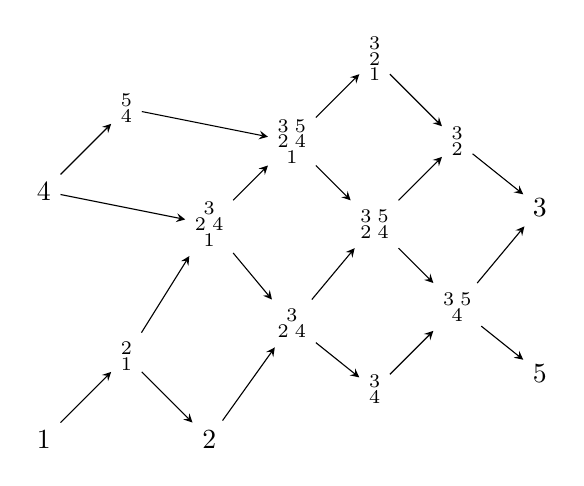
\begin{tikzpicture}[scale=1.05,>=stealth]
    \node (a11) at (0,0) {$1$};
    \node (a44) at (0,3) {$4$};

    \node (a12) at (1,1) {$\substack{2\\1}$};
    \node (a45) at (1,4) {$\substack{5\\4}$};

    \node (a14) at (2,2.6) {$\substack{3\\2\;4\\1}$};
    \node (a22) at (2,0) {$2$};

    \node (a15) at (3,3.6) {$\substack{3\;5\\2\;4\\1}$};
    \node (a24) at (3,1.4) {$\substack{3\\2\;4}$};

    \node (a13) at (4,4.6) {$\substack{3\\2\\1}$};
    \node (a25) at (4,2.6) {$\substack{3\;5\\2\;4}$};
    \node (a34) at (4,0.6) {$\substack{3\\4}$};

    \node (a23) at (5,3.6) {$\substack{3\\2}$};
    \node (a35) at (5,1.6) {$\substack{3\;5\\4}$};

    \node (a33) at (6,2.8) {$3$};
    \node (a55) at (6,0.8) {$5$};

    \draw[->] (a11) -- (a12);
    \draw[->] (a12) -- (a14);
    \draw[->] (a12) -- (a22);
    \draw[->] (a44) -- (a14);
    \draw[->] (a44) -- (a45);
    \draw[->] (a45) -- (a15);

    \draw[->] (a14) -- (a15);
    \draw[->] (a14) -- (a24);
    \draw[->] (a22) -- (a24);

    \draw[->] (a15) -- (a13);
    \draw[->] (a15) -- (a25);
    \draw[->] (a24) -- (a25);
    \draw[->] (a24) -- (a34);

    \draw[->] (a13) -- (a23);
    \draw[->] (a25) -- (a23);
    \draw[->] (a25) -- (a35);
    \draw[->] (a34) -- (a35);

    \draw[->] (a23) -- (a33);
    \draw[->] (a35) -- (a33);
    \draw[->] (a35) -- (a55);
    \end{tikzpicture}
    \]
    The left boundary consists of projective representations, while the right boundary
    consists of injective representations.
    \end{example}

    \begin{example}
    For the same quiver
    \[
    \begin{tikzcd}
    1 & 2 \arrow[l] & 3 \arrow[l] \arrow[r] & 4 & 5 \arrow[l],
    \end{tikzcd}
    \]
    consider the simple representation \(S(3)=3\). Since vertex \(3\) is a source, we have
    \[
        I(3)=S(3).
    \]
    Hence
    \[
        \tau^{-1}S(3)=0.
    \]
    On the projective side, a minimal projective resolution of \(S(3)\) is
    \[
        0
        \longrightarrow
        \operatorname{rad}P(3)
        \longrightarrow
        P(3)
        \longrightarrow
        S(3)
        \longrightarrow
        0.
    \]
    Here
    \[
        \operatorname{rad}P(3)
        =
        P(2)\oplus P(4)
        =
        \substack{2\\1}
        \oplus
        4.
    \]
    Applying the Nakayama functor gives
    \[
        I(2)\oplus I(4)
        \longrightarrow
        I(3)
        \longrightarrow
        \nu S(3)
        \longrightarrow
        0.
    \]
    \end{example}

    \chapter{Lecture 11}

    \section{\texorpdfstring{\(\tau\)-Orbits}{tau-Orbits}}

Let \(Q\) be a quiver of Dynkin type \(A_n\). Recall that the Auslander--Reiten
translation is denoted by
\[
    \tau.
\]
In the Auslander--Reiten quiver, \(\tau\) is the translation which sends the
rightmost point of a mesh to the leftmost point of the same mesh.

\begin{definition}[\(\tau\)-orbit]
    Let \(M\) be an indecomposable representation. The \(\tau\)-orbit of \(M\) is
    the collection of indecomposable representations obtained from \(M\) by
    repeatedly applying \(\tau\) and \(\tau^{-1}\), whenever these are defined.
\end{definition}

Thus \(\tau^{-1}\) can be thought of as the translation to the right in the
Auslander--Reiten quiver.

\subsection{First Method: Auslander--Reiten Translation}

Let \(M\) be an indecomposable representation which is not injective. We want to
compute the translate to the right,
\[
    \tau^{-1}M.
\]

Start with an injective resolution
\[
    0
    \longrightarrow
    M
    \longrightarrow
    I_0
    \xrightarrow{g}
    I_1
    \longrightarrow
    0.
\]
Applying the inverse Nakayama functor \(\nu^{-1}\), which maps each
indecomposable injective representation \(I(j)\) to the corresponding
indecomposable projective representation \(P(j)\), we obtain a projective
presentation of \(\tau^{-1}M\):
\[
    0
    \longrightarrow
    \nu^{-1}I_0
    \xrightarrow{\nu^{-1}(g)}
    \nu^{-1}I_1
    \longrightarrow
    \tau^{-1}M
    \longrightarrow
    0.
\]

\begin{example}
    Consider the quiver
    \[
    Q:
    \begin{tikzcd}[column sep=large]
        1 & 2 \arrow[l] & 3 \arrow[l] \arrow[r] & 4 & 5 \arrow[l]
    \end{tikzcd}
    \]
    and let
    \[
        M=4.
    \]
    An injective resolution of \(M\) is
    \[
        0
        \longrightarrow
        4
        \longrightarrow
        \begin{array}{ccc}
            3 && 5\\[-1mm]
            &4&
        \end{array}
        \longrightarrow
        3\oplus 5
        \longrightarrow
        0.
    \]
    Applying \(\nu^{-1}\), we obtain
    \[
        0
        \longrightarrow
        4
        \longrightarrow
        \begin{array}{ccc}
            &3&\\[-1mm]
            2&&4\\[-1mm]
            1&&
        \end{array}
        \oplus
        \begin{array}{c}
            5\\[-1mm]
            4
        \end{array}
        \longrightarrow
        \begin{array}{ccc}
            3&&5\\[-1mm]
            2&&4\\[-1mm]
            1&&
        \end{array}
        \longrightarrow
        0.
    \]
    Hence
    \[
        \tau^{-1}M
        =
        \tau^{-1}4
        =
        \begin{array}{ccc}
            3&&5\\[-1mm]
            2&&4\\[-1mm]
            1&&
        \end{array}.
    \]
\end{example}

\subsection{Second Method: Coxeter Functor}

Choose a sequence of vertices
\[
    (i_1,i_2,\dots,i_n)
\]
such that \(i_r\neq i_s\) for \(r\neq s\), as follows:

\begin{enumerate}
    \item \(i_1\) is a sink of \(Q\).
    \item \(i_2\) is a sink of the quiver \(s_{i_2}Q\), obtained from \(Q\) by
    reversing all arrows incident to \(i_1\).
    \item More generally, \(i_t\) is a sink of
    \[
        s_{i_{t-1}}\cdots s_{i_2}s_{i_1}Q,
        \qquad t=2,\dots,n.
    \]
\end{enumerate}

For the quiver
\[
    \begin{tikzcd}[column sep=large]
        1 & 2 \arrow[l] & 3 \arrow[l] \arrow[r] & 4 & 5 \arrow[l]
    \end{tikzcd}
\]
one possible choice is
\[
    (1,4,2,3,5).
\]

Next define reflections
\[
    s_i:\mathbb{R}^n\longrightarrow \mathbb{R}^n
\]
by
\[
    s_i(x)=x-2B(x,e_i)e_i,
\]
where \(e_1,\dots,e_n\) is the standard basis of \(\mathbb{R}^n\), and \(B\) is
the symmetric bilinear form determined by
\[
    B(e_i,e_j)=
    \begin{cases}
        1, & i=j,\\[1mm]
        -\dfrac{1}{2}, & i \text{ is adjacent to } j \text{ in } Q,\\[2mm]
        0, & \text{otherwise}.
    \end{cases}
\]

Equivalently, if
\[
    x=\sum_j a_j e_j,
\]
then
\[
    s_i(x)=\sum_j a'_j e_j,
\]
where
\[
    a'_j=a_j \quad \text{for } j\neq i,
\]
and
\[
    a'_i=-a_i+\sum_{j\sim i}a_j.
\]
Here \(j\sim i\) means that \(j\) is adjacent to \(i\) in the underlying graph of
\(Q\).

\begin{definition}[Coxeter element]
    The Coxeter element associated with the chosen sequence
    \((i_1,\dots,i_n)\) is
    \[
        c=s_{i_1}s_{i_2}\cdots s_{i_n}.
    \]
\end{definition}

For the running example,
\[
    c=s_1s_4s_2s_3s_5.
\]

This Coxeter element can be used to compute the dimension vector of
\(\tau^{-1}M\). If
\[
    \dim M=(d_1,\dots,d_n),
\]
and
\[
    c\left(\sum_i d_i e_i\right)=\sum_i d'_i e_i,
\]
then
\[
    \dim(\tau^{-1}M)=(d'_1,\dots,d'_n).
\]

\begin{example}
    Let \(M=4\). Then
    \[
        \dim M=(0,0,0,1,0),
    \]
    hence
    \[
        \dim M=e_4.
    \]
    Applying the Coxeter element, we get
    \[
    \begin{aligned}
        c(e_4)
        &=s_1s_4s_2s_3s_5(e_4)\\
        &=s_1s_4s_2s_3(e_4+e_5)\\
        &=s_1s_4s_2(e_3+e_4+e_5)\\
        &=s_1s_4(e_2+e_3+e_4+e_5)\\
        &=s_1(e_2+e_3+e_4+e_5)\\
        &=e_1+e_2+e_3+e_4+e_5.
    \end{aligned}
    \]
    Therefore
    \[
        \dim(\tau^{-1}M)=(1,1,1,1,1),
    \]
    and hence
    \[
        \tau^{-1}4
        =
        \begin{array}{ccc}
            3&&5\\[-1mm]
            2&&4\\[-1mm]
            1&&
        \end{array}.
    \]
\end{example}

\begin{remark}[Cartan matrix method]
    An equivalent method uses the Cartan matrix \(C\) of the quiver \(Q\).
    The Cartan matrix is defined by
    \[
        C=(c_{ij}),
        \qquad
        c_{ij}=\#\{\text{paths from }j\text{ to }i\}.
    \]
    If \(Q\) has no oriented cycles, then \(C\) is invertible. The Coxeter matrix
    is
    \[
        \Phi=-C^tC^{-1},
    \]
    and its inverse is
    \[
        \Phi^{-1}=-C(C^{-1})^t.
    \]
    For an indecomposable non-injective representation \(M\), one has
    \[
        \Phi^{-1}\dim M=\dim(\tau^{-1}M).
    \]
\end{remark}

\section{Diagonals of a Polygon with \texorpdfstring{\(n+3\)}{n+3} Vertices}

We now describe a geometric model for the Auslander--Reiten quiver of type
\(A_n\).

Start with a regular polygon with \(n+3\) vertices.

\begin{definition}[Diagonal]
    A diagonal of the polygon is a straight line segment joining two vertices of
    the polygon and passing through the interior of the polygon.
\end{definition}

\begin{definition}[Triangulation]
    A triangulation of the polygon is a maximal collection of pairwise non-crossing
    diagonals. Such a collection cuts the polygon into triangles.
\end{definition}

Given a triangle with sides \(a,b,c\), we say that the side \(a\) is clockwise from
the side \(b\) if, when one travels along the boundary of the triangle in the
clockwise direction, the sides occur in the repeating order
\[
    a,b,c,a,b,c,\dots.
\]

\subsection{Constructing a Triangulation from a Quiver}

Let \(Q\) be a quiver of type \(A_n\). We construct a triangulation \(T_Q\) of an
\((n+3)\)-gon as follows.

Choose a vertex \(1\) of \(Q\) with only one neighbor. Draw a diagonal cutting
off a triangle and label this diagonal by \(1\).

Suppose that the next vertex is \(2\).

\begin{itemize}
    \item If
    \[
        1\longleftarrow 2
    \]
    is an arrow in \(Q\), then draw the unique diagonal labelled \(2\) such that
    the diagonals \(1,2\) and one boundary segment form a triangle, with diagonal
    \(2\) clockwise from diagonal \(1\).

    \item If
    \[
        1\longrightarrow 2
    \]
    is an arrow in \(Q\), then draw the unique diagonal labelled \(2\) such that
    the diagonals \(1,2\) and one boundary segment form a triangle, with diagonal
    \(2\) counterclockwise from diagonal \(1\).
\end{itemize}

Continue this procedure inductively until all diagonals
\[
    1,2,\dots,n
\]
have been constructed. The resulting triangulation is denoted by \(T_Q\).

\begin{example}
    For the quiver
    \[
    Q:
    \begin{tikzcd}[column sep=large]
        1 & 2 \arrow[l] & 3 \arrow[l] \arrow[r] & 4 & 5 \arrow[l]
    \end{tikzcd}
    \]
    the construction gives a triangulation of an octagon, since here
    \[
        n=5,
        \qquad
        n+3=8.
    \]
\end{example}

\subsection{Diagonals and Indecomposable Representations}

Let \(\gamma\) be a diagonal of the polygon which does not belong to the fixed
triangulation \(T_Q\). Since \(T_Q\) is a triangulation, the diagonal \(\gamma\)
crosses a certain set of diagonals in \(T_Q\).

Moreover, \(\gamma\) is uniquely determined by the set of diagonals in \(T_Q\)
which it crosses.

To such a diagonal \(\gamma\), we associate a representation
\[
    M_\gamma=(M_i,\varphi_\alpha)
\]
of \(Q\) as follows:
\[
    M_i=
    \begin{cases}
        k, & \gamma \text{ crosses the diagonal labelled } i,\\
        0, & \text{otherwise}.
    \end{cases}
\]
For each arrow \(\alpha:i\to j\) in \(Q\), define
\[
    \varphi_\alpha:M_i\longrightarrow M_j
\]
by
\[
    \varphi_\alpha=
    \begin{cases}
        \operatorname{id}_k, & M_i=M_j=k,\\
        0, & \text{otherwise}.
    \end{cases}
\]

This gives a bijection
\[
    \left\{
    \begin{array}{c}
        \text{diagonals not belonging}\\
        \text{to }T_Q
    \end{array}
    \right\}
    \longleftrightarrow
    \left\{
    \begin{array}{c}
        \text{isomorphism classes of}\\
        \text{indecomposable representations of }Q
    \end{array}
    \right\}.
\]

\subsection{Auslander--Reiten Translation in the Polygon Model}

In the polygon model, the Auslander--Reiten translation \(\tau\) is given by
elementary clockwise rotation of the polygon.

Equivalently, if \(\gamma\) is a diagonal, then \(\tau\gamma\) is obtained by
rotating both endpoints of \(\gamma\) one step clockwise.

If \(\gamma_i\) denotes the diagonal labelled \(i\) in the triangulation \(T_Q\),
then the projective and injective representations are given by
\[
    P(i)=M_{\tau^{-1}\gamma_i},
    \qquad
    I(i)=M_{\tau\gamma_i}.
\]

Thus the whole Auslander--Reiten quiver may be constructed geometrically by
starting with the projective diagonals and repeatedly applying clockwise rotation.

\subsection{Counting Diagonals}

An \((n+3)\)-gon has
\[
    \frac{(n+3)n}{2}
\]
diagonals.

Indeed, each of the \(n+3\) vertices can be joined to \(n\) non-adjacent vertices,
and each diagonal is counted twice. Hence the number of diagonals is
\[
    \frac{(n+3)n}{2}.
\]

For example, when \(n=5\), the polygon has \(8\) vertices, and the number of
diagonals is
\[
    \frac{8\cdot 5}{2}=20.
\]

Since a triangulation of an \((n+3)\)-gon contains exactly \(n\) diagonals, the
number of diagonals not in \(T_Q\) is
\[
    \frac{(n+3)n}{2}-n
    =
    \frac{n(n+1)}{2}.
\]
Therefore the number of indecomposable representations of a quiver of type
\(A_n\) is
\[
    \frac{n(n+1)}{2}.
\]

\chapter{Lecture 12}

% Requires:
% \usepackage{amsmath,amssymb,amsthm}
% \usepackage{tikz}
% \usetikzlibrary{arrows.meta,positioning}

\section{Computing Dimensions and Short Exact Sequences}

Let \(M\) and \(N\) be two indecomposable representations. We want to obtain
information about the vector space
\[
    \operatorname{Hom}(M,N).
\]
The Auslander--Reiten quiver allows us to compute the dimension of this space
quite efficiently, at least when \(M\) and \(N\) lie in the same connected component
of the Auslander--Reiten quiver.

\subsection{Dimension of \texorpdfstring{\(\operatorname{Hom}(M,N)\)}{Hom(M,N)}}

Let \(Q\) be a quiver of type \(A\), and let \(M,N\) be two indecomposable
representations of \(Q\). We can compute
\[
    \dim_k \operatorname{Hom}(M,N)
\]
from the relative positions of \(M\) and \(N\) in the Auslander--Reiten quiver.

We first introduce some terminology.

\begin{definition}[Sectional path]
    A path
    \[
        M_0 \longrightarrow M_1 \longrightarrow \cdots \longrightarrow M_s
    \]
    in the Auslander--Reiten quiver is called a \textbf{sectional path} if
    \[
        \tau M_{i+1} \neq M_{i-1}
        \qquad
        \text{for all } i=1,\dots,s-1.
    \]
\end{definition}

\begin{definition}
    Let \(M\) be an indecomposable representation.
    We denote by
    \[
        \Sigma_{\rightarrow}(M)
    \]
    the set of all indecomposable representations which can be reached from \(M\)
    by a sectional path.

    Dually, we denote by
    \[
        \Sigma_{\leftarrow}(M)
    \]
    the set of all indecomposable representations from which one can reach \(M\)
    by a sectional path.
\end{definition}

\begin{definition}[Maximal slanted rectangle]
    Let \(M\) be an indecomposable representation. We denote by
    \[
        R_{\rightarrow}(M)
    \]
    the set of all indecomposable representations whose positions in the
    Auslander--Reiten quiver lie in the maximal slanted rectangular region whose
    left boundary is \(\Sigma_{\rightarrow}(M)\).

    Equivalently, \(R_{\rightarrow}(M)\) is the maximal slanted rectangle in the
    Auslander--Reiten quiver whose leftmost point is \(M\).
\end{definition}

Schematically, one should think of \(R_{\rightarrow}(M)\) as follows:
\[
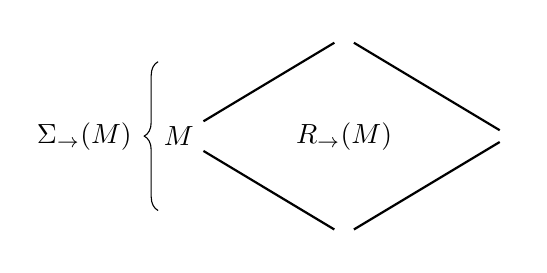
\begin{tikzpicture}[scale=1.05,>=Stealth]
    \node (M) at (-2,0) {\(M\)};
    \node (a) at (0,1.2) {};
    \node (b) at (2,0) {};
    \node (c) at (0,-1.2) {};

    \draw[thick] (M) -- (a) -- (b) -- (c) -- (M);
    \draw[decorate,decoration={brace,amplitude=5pt}] (-2.25,-0.9) -- (-2.25,0.9)
        node[midway,left=6pt] {\(\Sigma_{\rightarrow}(M)\)};
    \node at (0,0) {\(R_{\rightarrow}(M)\)};
\end{tikzpicture}
\]

\begin{theorem}[Hom dimensions in type \(A\)]
    Let \(Q\) be a quiver of type \(A\), and let \(M,N\) be indecomposable
    representations of \(Q\). Then
    \[
        \dim_k \operatorname{Hom}(M,N)
        \in \{0,1\}.
    \]
    More precisely,
    \[
        \dim_k \operatorname{Hom}(M,N)=1
    \]
    if and only if
    \[
        N\in R_{\rightarrow}(M).
    \]
    Otherwise,
    \[
        \dim_k \operatorname{Hom}(M,N)=0.
    \]
\end{theorem}

\begin{example}
    For \(M=P(4)\), the Auslander--Reiten quiver can be labelled by numbers
    \(0\) and \(1\), where the number at the vertex corresponding to an
    indecomposable representation \(N\) is
    \[
        \dim_k \operatorname{Hom}(M,N).
    \]
    The vertex corresponding to \(M=P(4)\) itself is the leftmost vertex labelled
    by \(1\), since
    \[
        \operatorname{Hom}(M,M)\cong k.
    \]
\end{example}

\begin{example}
    For \(M=S(2)\), the region \(R_{\rightarrow}(M)\) degenerates to a single
    sectional line in the Auslander--Reiten quiver. The labels \(0\) and \(1\)
    again indicate the dimensions
    \[
        \dim_k \operatorname{Hom}(M,N)
    \]
    for the corresponding indecomposable representations \(N\).
\end{example}

Symmetrically, we denote by
\[
    R_{\leftarrow}(N)
\]
the maximal slanted rectangle in the Auslander--Reiten quiver whose rightmost
point is \(N\). Then we can compute
\[
    \dim_k \operatorname{Hom}(-,N)
\]
using \(R_{\leftarrow}(N)\).

In particular, the computation of \(\dim_k\operatorname{Hom}(P(4),-)\) also gives
the computation of
\[
    \dim_k\operatorname{Hom}(-,I(4)),
\]
because the corresponding rectangles coincide.

\begin{remark}
    If \(M=P(i)\) is an indecomposable projective representation, then by the
    standard isomorphism
    \[
        \operatorname{Hom}(P(i),N)\cong N_i,
    \]
    the representations in \(R_{\rightarrow}(P(i))\) are precisely the
    indecomposable representations \(N\) such that
    \[
        N_i\neq 0.
    \]

    Dually, using
    \[
        \operatorname{Hom}(M,I(i))\cong M_i,
    \]
    there is a unique rightmost point in \(R_{\rightarrow}(P(i))\), namely the
    position of the indecomposable injective representation \(I(i)\). Hence
    \[
        R_{\rightarrow}(P(i))
        =
        R_{\leftarrow}(I(i)).
    \]
\end{remark}

\subsection{Dimension of \texorpdfstring{\(\operatorname{Ext}^1(M,N)\)}{Ext1(M,N)}}

We now consider
\[
    \operatorname{Ext}^1(M,N).
\]

If \(M\) is projective, then
\[
    \operatorname{Ext}^1(M,N)=0.
\]
Therefore, we assume that \(M\) is not projective. In this case \(\tau M\) is
defined and appears as a vertex in the Auslander--Reiten quiver.

The Auslander--Reiten formula gives an isomorphism
\[
    \operatorname{Ext}^1(M,N)
    \cong
    D\operatorname{Hom}(N,\tau M),
\]
where
\[
    D=\operatorname{Hom}_k(-,k)
\]
is the \(k\)-linear duality.

Therefore
\[
    \dim_k \operatorname{Ext}^1(M,N)
    =
    \dim_k \operatorname{Hom}(N,\tau M).
\]

Thus the dimension of
\[
    \operatorname{Ext}^1(M,-)
\]
can be computed using the maximal slanted rectangle
\[
    R_{\leftarrow}(\tau M).
\]

\begin{example}
    For \(M=I(3)\), the dimensions of
    \[
        \operatorname{Ext}^1(M,N)
    \]
    are obtained by labelling the Auslander--Reiten quiver according to the
    maximal slanted rectangle ending at \(\tau M\). The labels \(0\) and \(1\)
    indicate whether
    \[
        \operatorname{Ext}^1(M,N)
    \]
    is zero or one-dimensional.
\end{example}

\subsection{Short Exact Sequences}

The elements of \(\operatorname{Ext}^1(M,N)\) can be represented by short exact
sequences of the form
\[
    0
    \longrightarrow
    N
    \longrightarrow
    E
    \longrightarrow
    M
    \longrightarrow
    0,
\]
where \(E\) is some representation of \(Q\).

Let \(M\) and \(N\) be indecomposable representations. We want to compute the
possible middle terms \(E\) occurring in such short exact sequences.

If
\[
    \dim_k \operatorname{Ext}^1(M,N)=0,
\]
then the only possibility is the split extension, namely
\[
    E\cong M\oplus N.
\]

If, on the other hand,
\[
    \dim_k \operatorname{Ext}^1(M,N)=1,
\]
then, up to isomorphism, there is exactly one other possibility for \(E\), namely
the middle term of the unique non-split extension.

For representations of type \(A\), this middle term \(E\) can be computed directly
from the relative positions of \(M\) and \(N\) in the Auslander--Reiten quiver.

\begin{proposition}[Middle terms from sectional paths]
    Let \(M,N\) be indecomposable representations of a quiver of type \(A\), and
    assume that
    \[
        \operatorname{Ext}^1(M,N)\neq 0.
    \]
    Then
    \[
        N\in R_{\leftarrow}(\tau M).
    \]
    Consequently, the sets
    \[
        \Sigma_{\rightarrow}(N)
        \qquad\text{and}\qquad
        \Sigma_{\leftarrow}(M)
    \]
    have either one or two points in common. These common points correspond
    exactly to the indecomposable direct summands of the middle term \(E\).
\end{proposition}

In pictures, we mark \(N\) by \(\ominus\) and \(M\) by \(\oplus\). The
representations in \(\Sigma_{\rightarrow}(N)\) are marked by \(-\), while the
representations in \(\Sigma_{\leftarrow}(M)\) are marked by \(+\). The points of
intersection are marked by \(\pm\). These intersection points give the
indecomposable summands of \(E\).

\begin{example}
    One possible configuration gives the short exact sequence
    \[
        0
        \longrightarrow
        \begin{matrix}
            5\\[-1mm]
            4
        \end{matrix}
        \longrightarrow
        \begin{matrix}
            3 & 5\\[-1mm]
              & 4
        \end{matrix}
        \longrightarrow
        3
        \longrightarrow
        0.
    \]
\end{example}

\begin{example}
    Another possible configuration gives the short exact sequence
    \[
        0
        \longrightarrow
        \begin{matrix}
            3 & 5\\[-1mm]
            2 & 4\\[-1mm]
            1 &
        \end{matrix}
        \longrightarrow
        \begin{matrix}
            3 & 5\\[-1mm]
              & 4
        \end{matrix}
        \oplus
        \begin{matrix}
            3\\[-1mm]
            2\\[-1mm]
            1
        \end{matrix}
        \longrightarrow
        3
        \longrightarrow
        0.
    \]
\end{example}

\section{Representation Type}

\begin{definition}[Finite representation type]
    A quiver \(Q\) is said to be of \textbf{finite representation type} if the
    number of isomorphism classes of indecomposable representations of \(Q\) is
    finite.
\end{definition}

It turns out that this classification depends only on the shape of the quiver and
not on the particular orientation of the arrows. We therefore introduce the following
notion.

\begin{definition}[Underlying graph]
    The \textbf{underlying graph} of a quiver \(Q\) is the unoriented graph obtained
    from \(Q\) by forgetting the directions of all arrows.
\end{definition}

\begin{theorem}[Gabriel's theorem]
    A connected quiver \(Q\) is of finite representation type if and only if its
    underlying graph is one of the Dynkin diagrams of type
    \[
        A_n,\qquad D_n,\qquad E_6,\qquad E_7,\qquad E_8.
    \]
\end{theorem}

\begin{remark}
    Dynkin diagrams also occur in several other classification problems in
    mathematics, for example in the classification of semisimple Lie algebras,
    root systems, Coxeter groups, and cluster algebras.
\end{remark}

\section{Auslander--Reiten Quivers of Type \texorpdfstring{\(D_n\)}{Dn}}

Let \(Q\) be a quiver of type \(D_n\). This means that the underlying unoriented
graph of \(Q\) is the Dynkin diagram of type \(D_n\):
\[
\begin{tikzpicture}[>=Stealth,scale=1]
    \node (1) at (0,0) {\(1\)};
    \node (2) at (1.2,0) {\(2\)};
    \node (dots) at (2.4,0) {\(\cdots\)};
    \node (n2) at (3.8,0) {\(n-2\)};
    \node (n1) at (5,0.7) {\(n-1\)};
    \node (n) at (5,-0.7) {\(n\)};

    \draw (1) -- (2);
    \draw (2) -- (dots);
    \draw (dots) -- (n2);
    \draw (n2) -- (n1);
    \draw (n2) -- (n);
\end{tikzpicture}
\]

\subsection{The Knitting Algorithm in Type \texorpdfstring{\(D_n\)}{Dn}}

For quivers of type \(D_n\), the knitting algorithm is similar to the type \(A\)
case, but there is a fourth type of mesh.

Besides the meshes occurring in type \(A\), we also have a mesh of the following
form:
\[
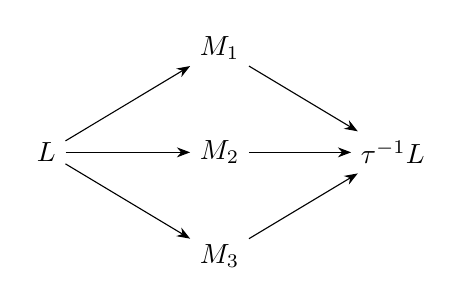
\begin{tikzpicture}[>=Stealth,scale=1.1]
    \node (L) at (0,0) {\(L\)};
    \node (M1) at (2,1.2) {\(M_1\)};
    \node (M2) at (2,0) {\(M_2\)};
    \node (M3) at (2,-1.2) {\(M_3\)};
    \node (T) at (4,0) {\(\tau^{-1}L\)};

    \draw[->] (L) -- (M1);
    \draw[->] (L) -- (M2);
    \draw[->] (L) -- (M3);

    \draw[->] (M1) -- (T);
    \draw[->] (M2) -- (T);
    \draw[->] (M3) -- (T);
\end{tikzpicture}
\]

In this case, the mesh relation for dimension vectors is
\[
    \dim L+\dim \tau^{-1}L
    =
    \dim M_1+\dim M_2+\dim M_3.
\]

Thus, once \(L,M_1,M_2,M_3\) are known, the dimension vector of
\(\tau^{-1}L\) is determined by
\[
    \dim \tau^{-1}L
    =
    \dim M_1+\dim M_2+\dim M_3-\dim L.
\]

\subsection{Indecomposable Representations of Type \texorpdfstring{\(D_n\)}{Dn}}

The isomorphism classes of indecomposable representations of quivers of type
\(D_n\) are determined by their dimension vectors
\[
    d=(d_1,\dots,d_n).
\]

The entries of such a dimension vector satisfy
\[
    d_i\in \{0,1,2\}.
\]

Moreover, if some entry \(d_i\) is equal to \(2\), then the following conditions hold:

\begin{enumerate}
    \item The vertex \(i\) is one of
    \[
        2,3,\dots,n-2.
    \]

    \item For every vertex \(j\) satisfying
    \[
        i\leq j\leq n-2,
    \]
    one has
    \[
        d_j=2.
    \]

    \item One has
    \[
        d_{i-1}\geq 1,
        \qquad
        d_{n-1}=d_n=1.
    \]
\end{enumerate}

Thus the vertices \(i\) with \(d_i=2\) form a subgraph of type \(A\) containing
the vertex \(n-2\).

The vertices \(i\neq n-1,n\) with \(d_i=1\) also form a subgraph of type \(A\).
If no entry \(d_j\) is equal to \(2\), then all vertices \(i\) with \(d_i=1\) form
a subgraph of type \(A\) or a subgraph of type \(D\).

Graphically, some possible configurations have the following forms:
\[
\begin{tikzpicture}[>=Stealth,scale=1]
    \node (a1) at (0,0) {\(0\)};
    \node (a2) at (1,0) {\(\cdots\)};
    \node (a3) at (2,0) {\(0\)};
    \node (b1) at (3,0) {\(1\)};
    \node (b2) at (4,0) {\(\cdots\)};
    \node (b3) at (5,0) {\(1\)};
    \node (c1) at (6,0) {\(2\)};
    \node (c2) at (7,0) {\(\cdots\)};
    \node (c3) at (8,0) {\(2\)};
    \node (u) at (9,0.7) {\(1\)};
    \node (v) at (9,-0.7) {\(1\)};

    \draw (a1) -- (a2) -- (a3) -- (b1) -- (b2) -- (b3) -- (c1) -- (c2) -- (c3);
    \draw (c3) -- (u);
    \draw (c3) -- (v);
\end{tikzpicture}
\]
and
\[
\begin{tikzpicture}[>=Stealth,scale=1]
    \node (a1) at (0,0) {\(0\)};
    \node (a2) at (1,0) {\(\cdots\)};
    \node (a3) at (2,0) {\(0\)};
    \node (b1) at (3,0) {\(1\)};
    \node (b2) at (4,0) {\(\cdots\)};
    \node (b3) at (5,0) {\(1\)};
    \node (c1) at (6,0) {\(1\)};
    \node (c2) at (7,0) {\(\cdots\)};
    \node (c3) at (8,0) {\(1\)};
    \node (u) at (9,0.7) {\(1\)};
    \node (v) at (9,-0.7) {\(1\)};

    \draw (a1) -- (a2) -- (a3) -- (b1) -- (b2) -- (b3) -- (c1) -- (c2) -- (c3);
    \draw (c3) -- (u);
    \draw (c3) -- (v);
\end{tikzpicture}
\]

The corresponding representation is
\[
    M=(M_i,\varphi_\alpha),
\]
where
\[
    M_i=k^{d_i}.
\]

For an arrow \(\alpha\), the map
\[
    \varphi_\alpha:M_{s(\alpha)}\longrightarrow M_{t(\alpha)}
\]
is given as follows:

\[
    \varphi_\alpha=
    \begin{cases}
        \operatorname{id}, & d_{s(\alpha)}=d_{t(\alpha)},\\[1mm]
        0, & d_{s(\alpha)}=0 \text{ or } d_{t(\alpha)}=0.
    \end{cases}
\]

It remains to specify the maps between one-dimensional and two-dimensional
vector spaces.

Suppose that one of the entries \(d_i\) is equal to \(2\). Then there are exactly
three arrows connecting a vertex with dimension \(1\) to a vertex with dimension
\(2\).

Two of these arrows, denoted by
\[
    \beta_1,\beta_2,
\]
connect the vertex \(n-2\) with the vertices \(n-1\) and \(n\). The vector space
of dimension \(2\) is at the vertex \(n-2\).

The third arrow, denoted by
\[
    \alpha_i,
\]
connects the vertices \(i\) and \(i+1\), with the vector space of dimension \(2\)
at the vertex \(i+1\).

Consider the one-dimensional subspace of \(M_{i+1}\) defined by
\[
    \ell_1'=
    \begin{cases}
        \operatorname{Im}\varphi_{\alpha_i},
        & \text{if } \alpha_i \text{ points to } i+1,\\[1mm]
        \operatorname{Ker}\varphi_{\alpha_i},
        & \text{otherwise}.
    \end{cases}
\]
Transporting this subspace along the identity maps between the two-dimensional
vertices gives a one-dimensional subspace
\[
    \ell_1\subseteq M_{n-2}.
\]

Similarly, define
\[
    \ell_2=
    \begin{cases}
        \operatorname{Im}\varphi_{\beta_1},
        & \text{if } \beta_1 \text{ points to } n-2,\\[1mm]
        \operatorname{Ker}\varphi_{\beta_1},
        & \text{otherwise},
    \end{cases}
\]
and
\[
    \ell_3=
    \begin{cases}
        \operatorname{Im}\varphi_{\beta_2},
        & \text{if } \beta_2 \text{ points to } n-2,\\[1mm]
        \operatorname{Ker}\varphi_{\beta_2},
        & \text{otherwise}.
    \end{cases}
\]

The condition on the maps is that the three one-dimensional subspaces
\[
    \ell_1,\ell_2,\ell_3\subseteq M_{n-2}
\]
are pairwise distinct.

\begin{remark}
    This condition excludes the degenerate cases where two of the relevant
    one-dimensional subspaces coincide. In type \(D_n\), this is the extra feature
    which does not appear in type \(A_n\).
\end{remark}


\end{document}
